\documentclass[11pt]{article}
\usepackage[utf8]{inputenc}	% Para caracteres en español
\usepackage{amsmath,amsthm,amsfonts,amssymb,amscd}
\usepackage{multirow,booktabs}
\usepackage[table]{xcolor}
\usepackage{fullpage}
\usepackage{lastpage}
\usepackage{enumitem}
\usepackage{fancyhdr}
\usepackage{mathrsfs}
\usepackage{wrapfig}
\usepackage{setspace}
\usepackage{calc}
\usepackage{multicol}
\usepackage{cancel}
\usepackage[retainorgcmds]{IEEEtrantools}
\usepackage[margin=3cm]{geometry}
\usepackage{amsmath}
\newlength{\tabcont}
\setlength{\parindent}{0.0in}
\setlength{\parskip}{0.05in}
\usepackage{empheq}
\usepackage{framed}
\usepackage[most]{tcolorbox}
\usepackage{xcolor}
\colorlet{shadecolor}{orange!15}
\parindent 0in
\parskip 12pt
\geometry{margin=1in, headsep=0.25in}
\theoremstyle{definition}
\newtheorem{defn}{Definition}
\newtheorem{reg}{Rule}
\newtheorem{exer}{Exercise}
\newtheorem{note}{Note}
\graphicspath{
    {figures/},{figures/feynman_diagrams/single_qubit_cavity/},{figures/feynman_diagrams/two_qubit_cavity/}
}
\usepackage{graphicx}
\usepackage{makecell}
\usepackage{lscape}
\usepackage{graphbox}
\usepackage{braket}
\newcommand{\commute}[2]{\left[#1,#2\right]}

\begin{document}
\title{Cavity Coupling}

\thispagestyle{empty}

\maketitle

\section{Introduction}
\section{System}
\begin{align}\label{EQ:cavity_hamiltonian}
    H & = \sum_q H_q + H_{cav} + \sum_q V_q \nonumber                                                                                        \\
      & = -\frac{1}{2}\sum_q (\omega_\sigma \sigma_z + \omega_\tau \tau_z) + \hbar\omega_c a^\dagger a + \hbar g \sum_q (1+Z_q)(a+a^\dagger)
\end{align}
\section{Effective Coupling}

\begin{table}[]
    \centering
    \begin{tabular}{@{}ccc@{}}
        \toprule
        Diagram                                                          & Label                                 & Interaction Form                                                                                                                       \\ \midrule
        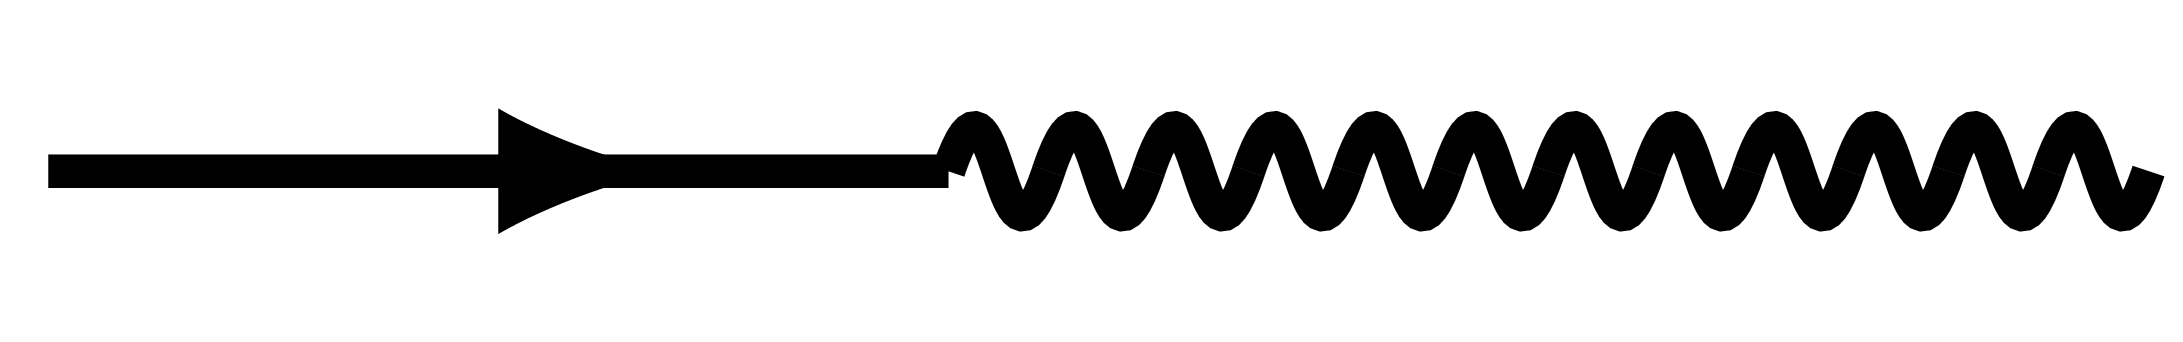
\includegraphics[align=c,width=1.2in]{A} & \makecell{$A_1$\\$A_2$}               & \makecell{$g_\tau\sigma_z\tau_-a^\dagger$ \\ $g_\sigma\sigma_-a^\dagger$}                                                              \\ \midrule
        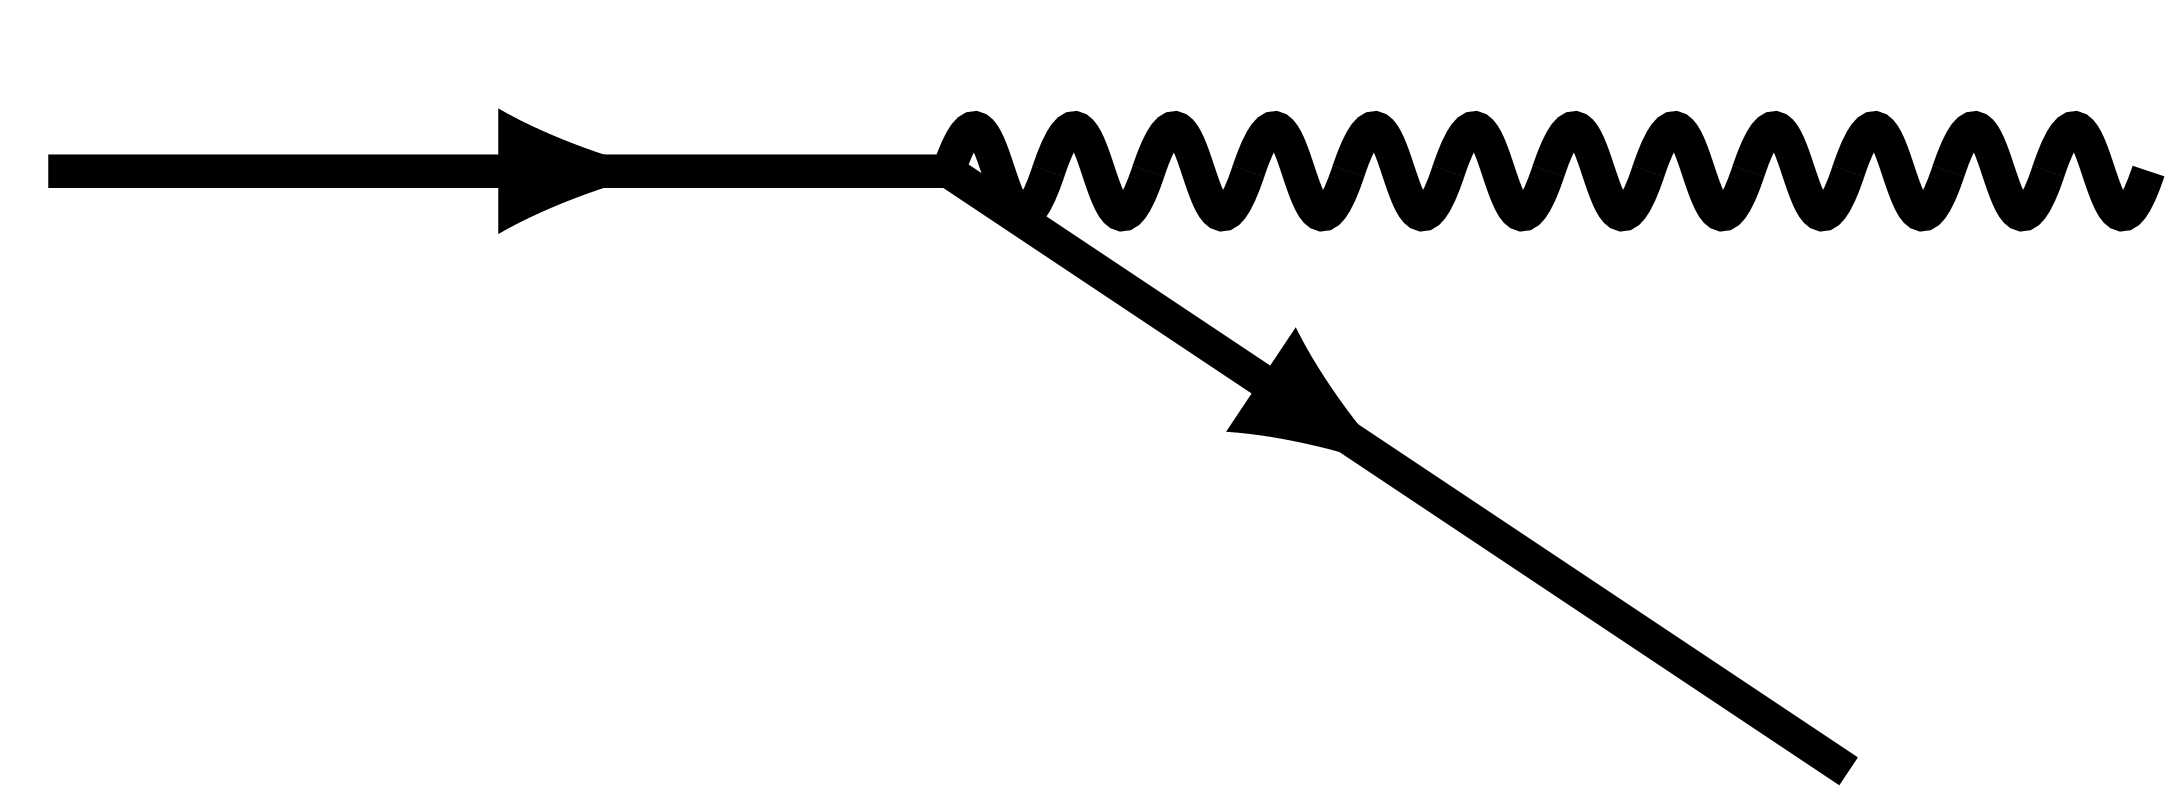
\includegraphics[align=c,width=1.2in]{B} & \makecell{$B_1$\\$B_2$}               & \makecell{$g_+\sigma_-\tau_+a^\dagger$ \\ $g_+\sigma_+\tau_-a^\dagger$}                                                                \\ \midrule
        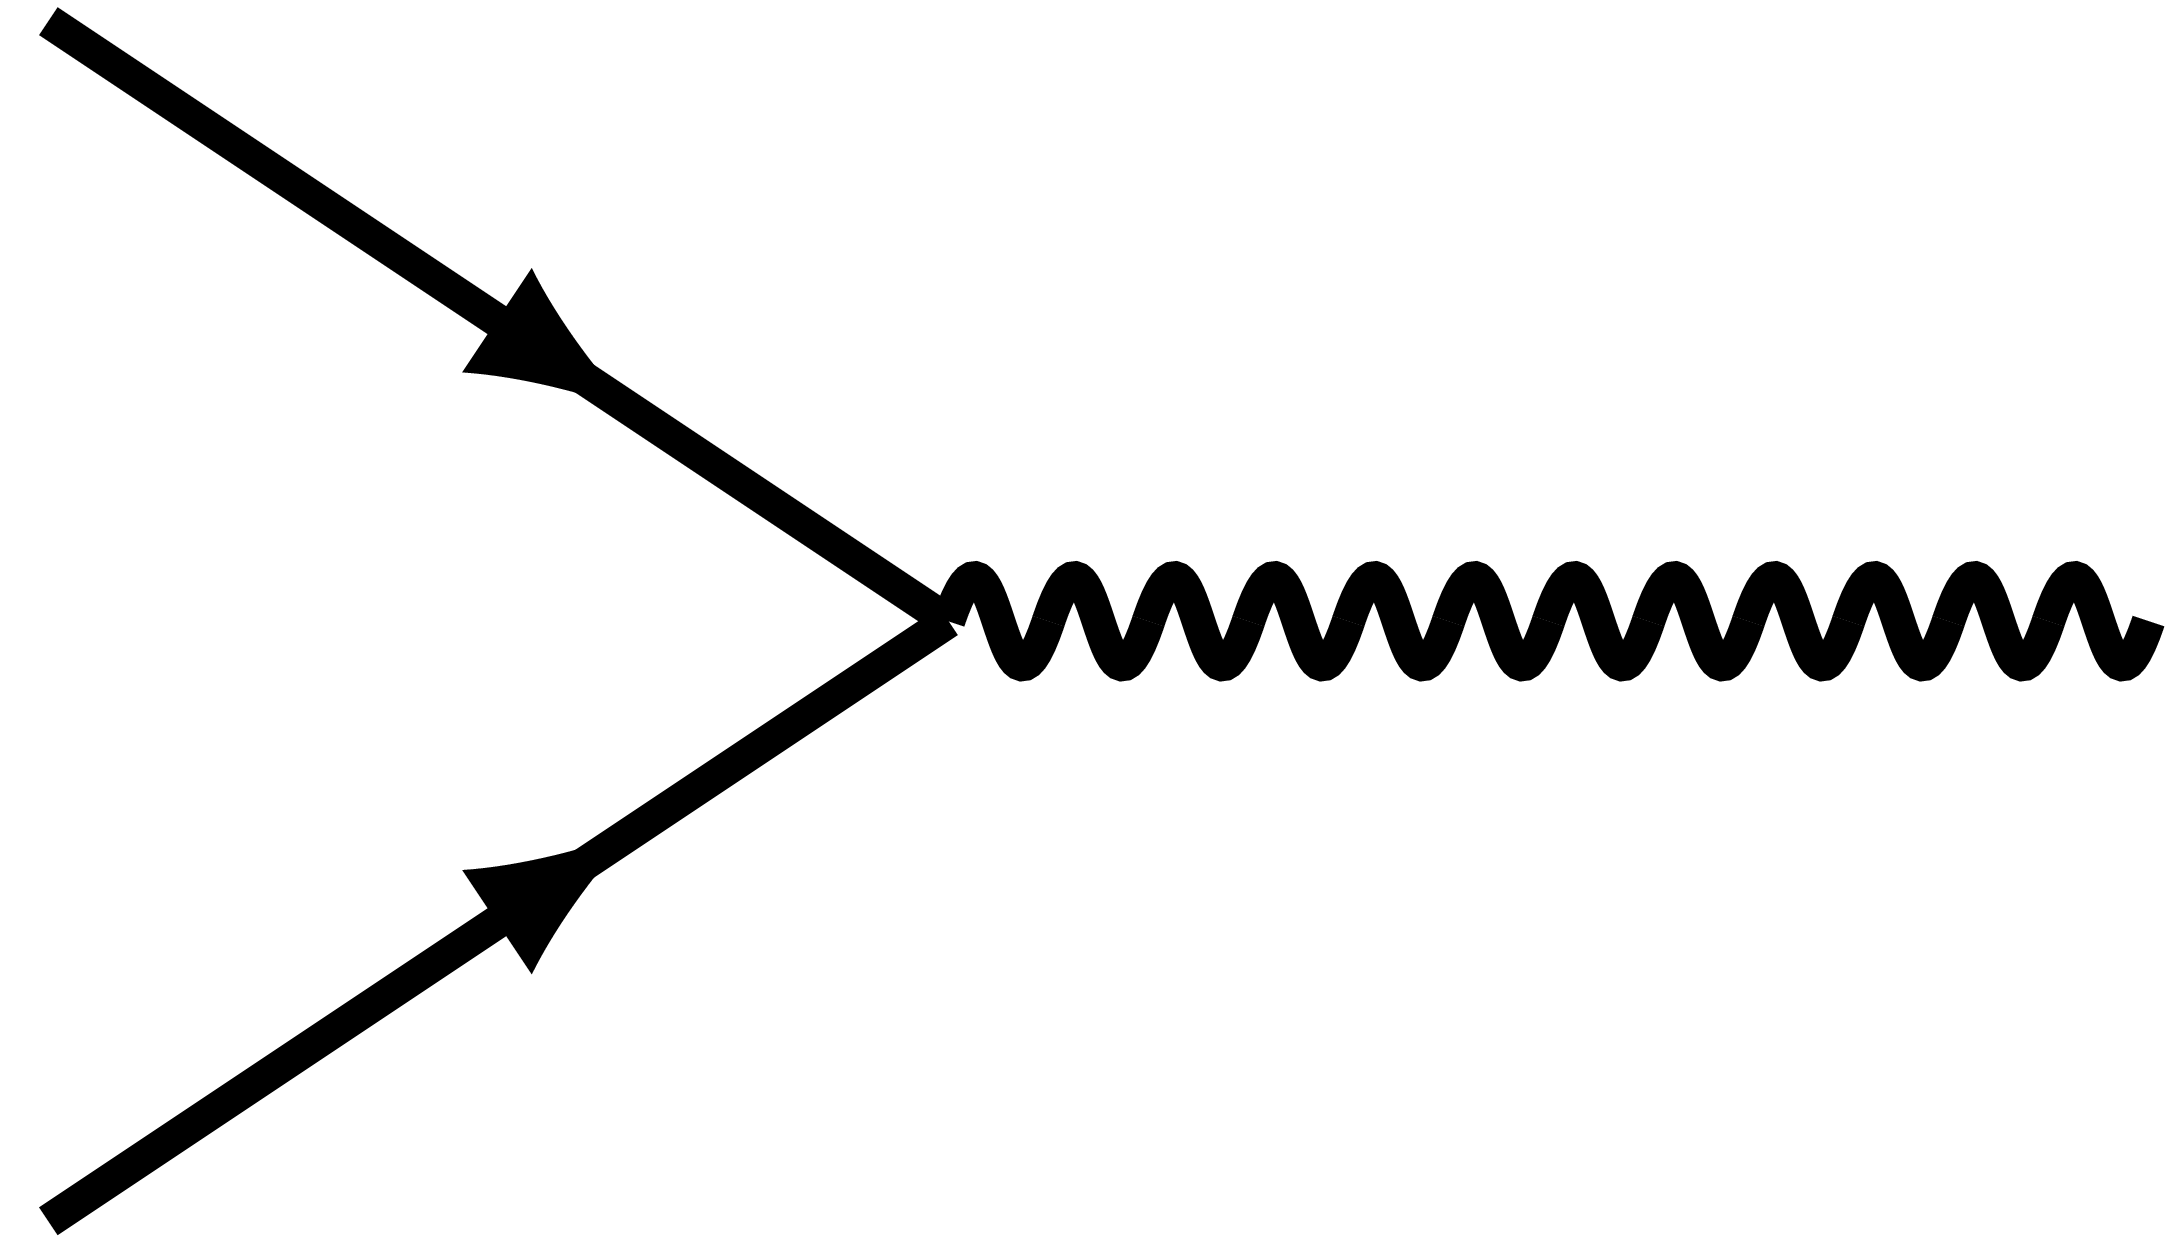
\includegraphics[align=c,width=1.2in]{C} & \makecell{$C_1$}                      & \makecell{$g_-\sigma_-\tau_-a^\dagger$}                                                                                                \\ \midrule
        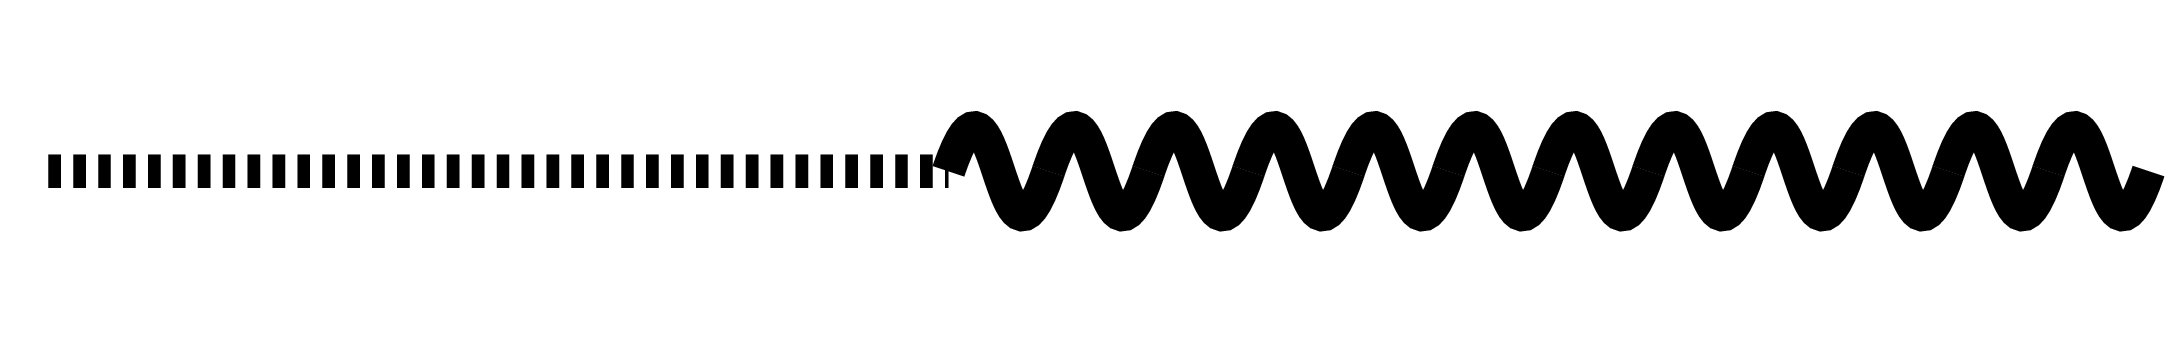
\includegraphics[align=c,width=1.2in]{D} & \makecell{$D_1$\\$D_2$\\$D_3$\\$D_4$} & \makecell{$ga^\dagger$ \\ $g_{\tau,z}\tau_za^\dagger$ \\ $g_{\sigma,z}\sigma_za^\dagger$ \\ $g_{\sigma\tau,z}\sigma_z\tau_za^\dagger$} \\ \midrule
        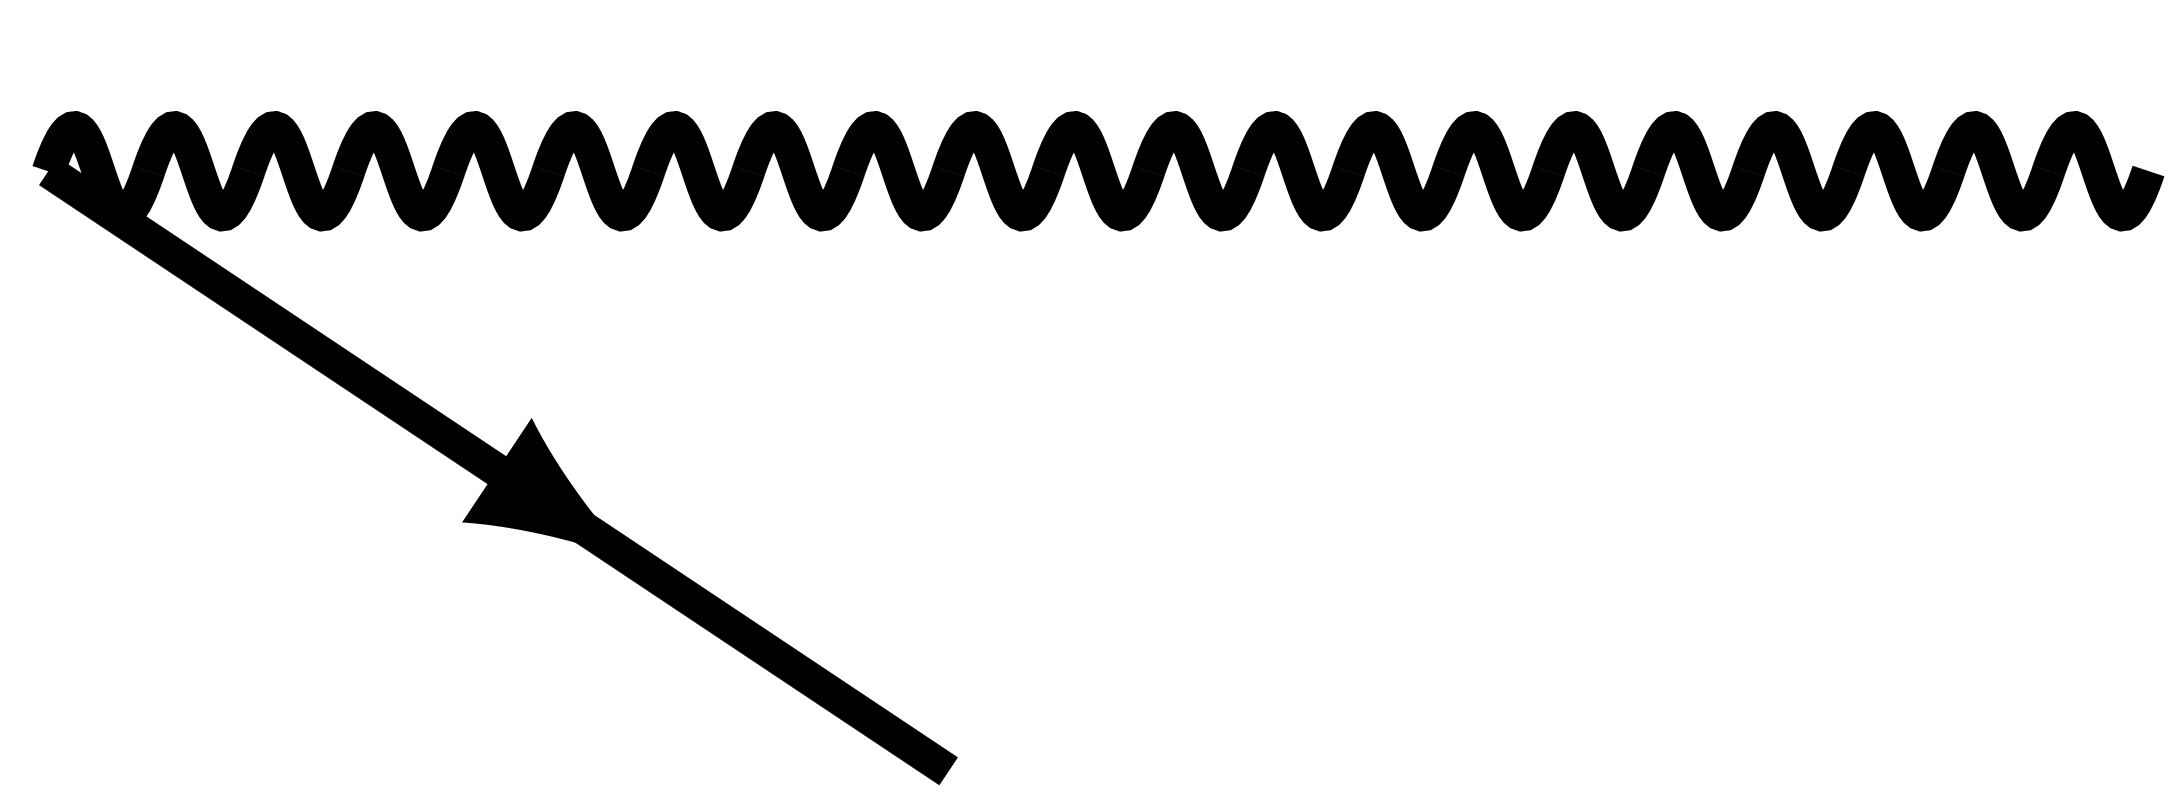
\includegraphics[align=c,width=1.2in]{E} & \makecell{$E_1$\\$E_2$}               & \makecell{$g_\tau\sigma_z\tau_+a^\dagger$ \\ $g_\sigma\sigma_+a^\dagger$}                                                              \\ \midrule
        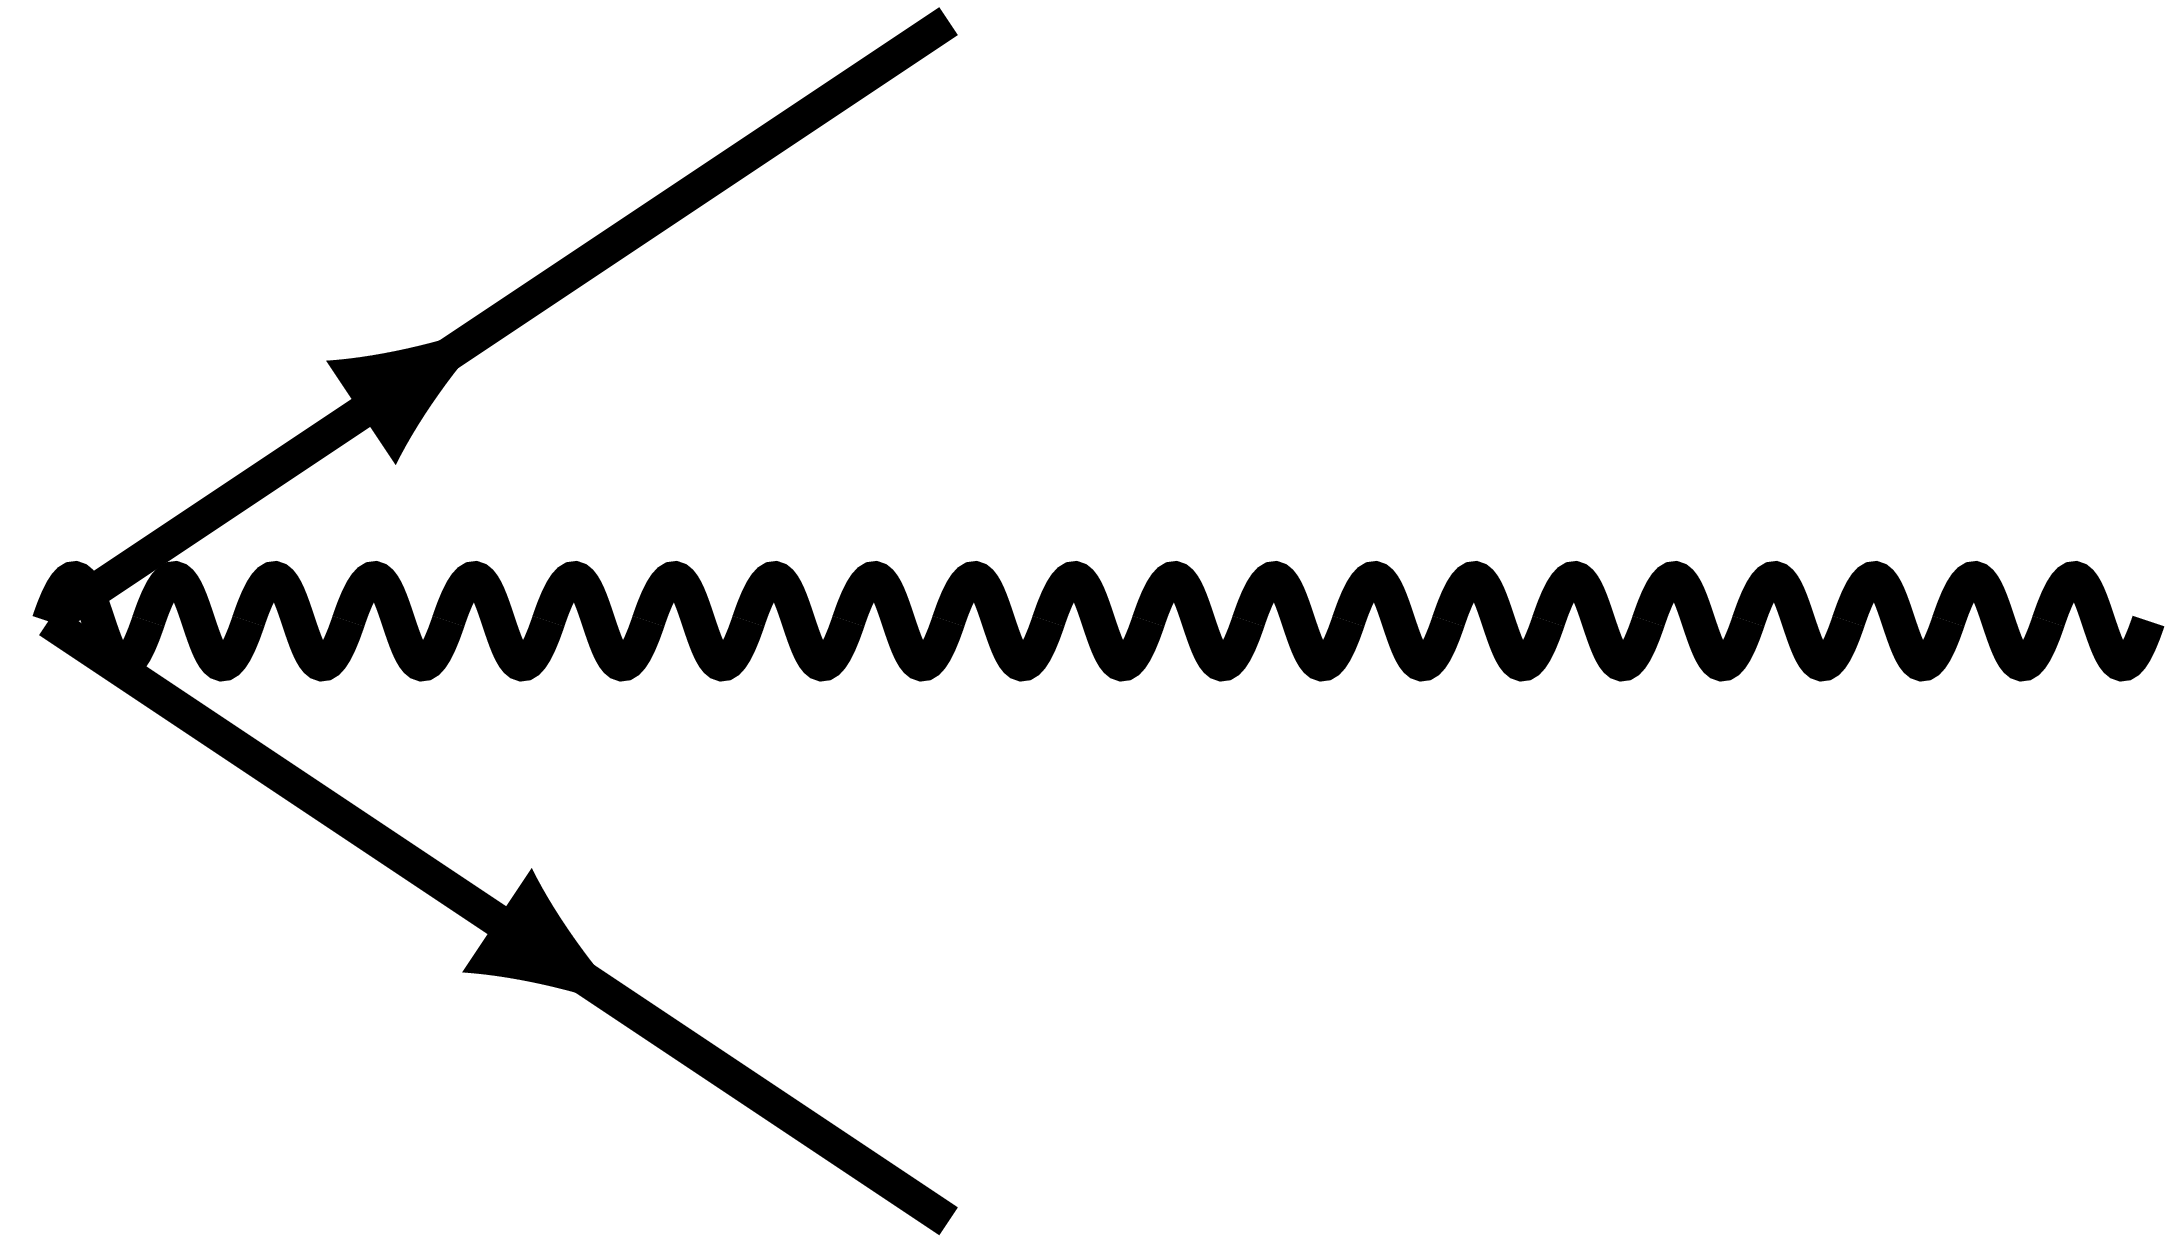
\includegraphics[align=c,width=1.2in]{F} & \makecell{$F_1$}                      & \makecell{$g_-\sigma_+\tau_+a^\dagger/2$}                                                                                              \\ \bottomrule
    \end{tabular}
    \caption[Single qubit cavity coupling terms]{
        Feynman-like diagrams depicting the coupling of the flip-flop qubit to the microwave cavity. 
        All diagrams show the creation of a photon. 
        The Hermitian conjugate diagrams (depicting photon annihilation) and their terms are not shown for brevity. 
        Arrows entering (leaving) the interaction point show the relaxation (excitation) of either the spin or the charge part of the qubit system, while a dashed line represents a phase shift with of the qubit system with no change in energy. 
        The diagrams are ordered roughly in terms of the strength of the interaction. 
        Notice that the $D$ to $F$ interactions have no possible avenue to conserve energy and thus are not important for single qubit coupling.
        These terms are the ones omitted when applying the rotating wave approximation.}
    \label{TAB:single_qubit_diagrams}
\end{table}

\begin{landscape}
    \begin{table}[]
        \centering
        \begin{tabular}{@{}r|cccccc@{}}
            & $A$ & $B$ & $C$ & $D$ & $E$ & $F$ \\ \midrule
        $A$ & 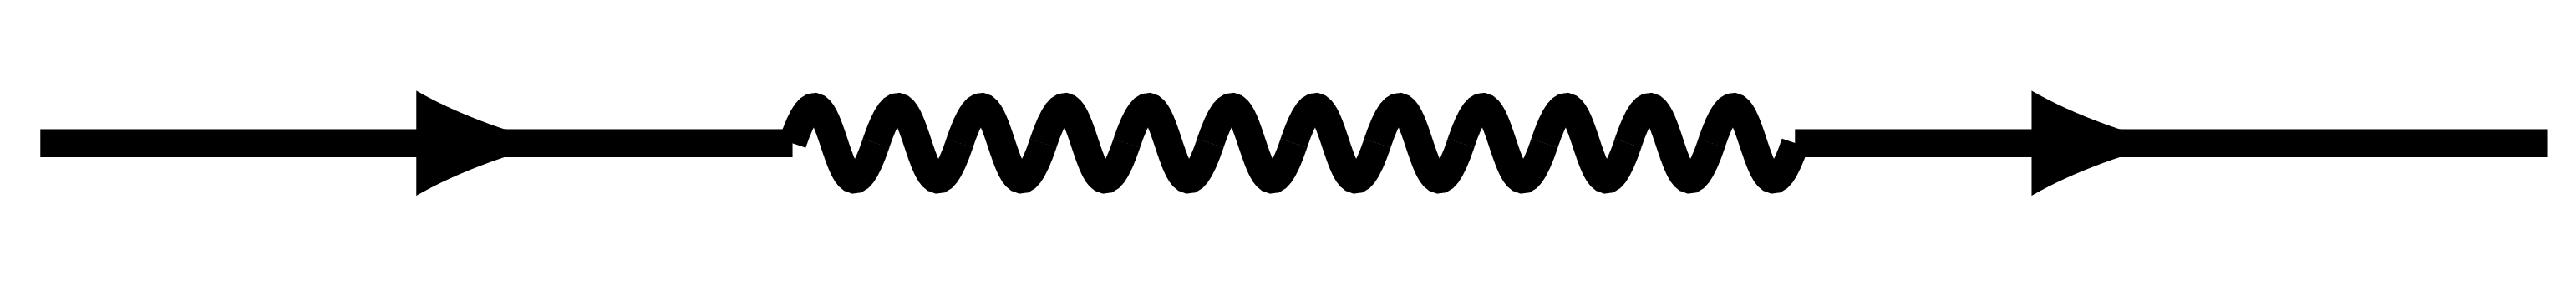
\includegraphics[align=c,width=1.2in]{AA}&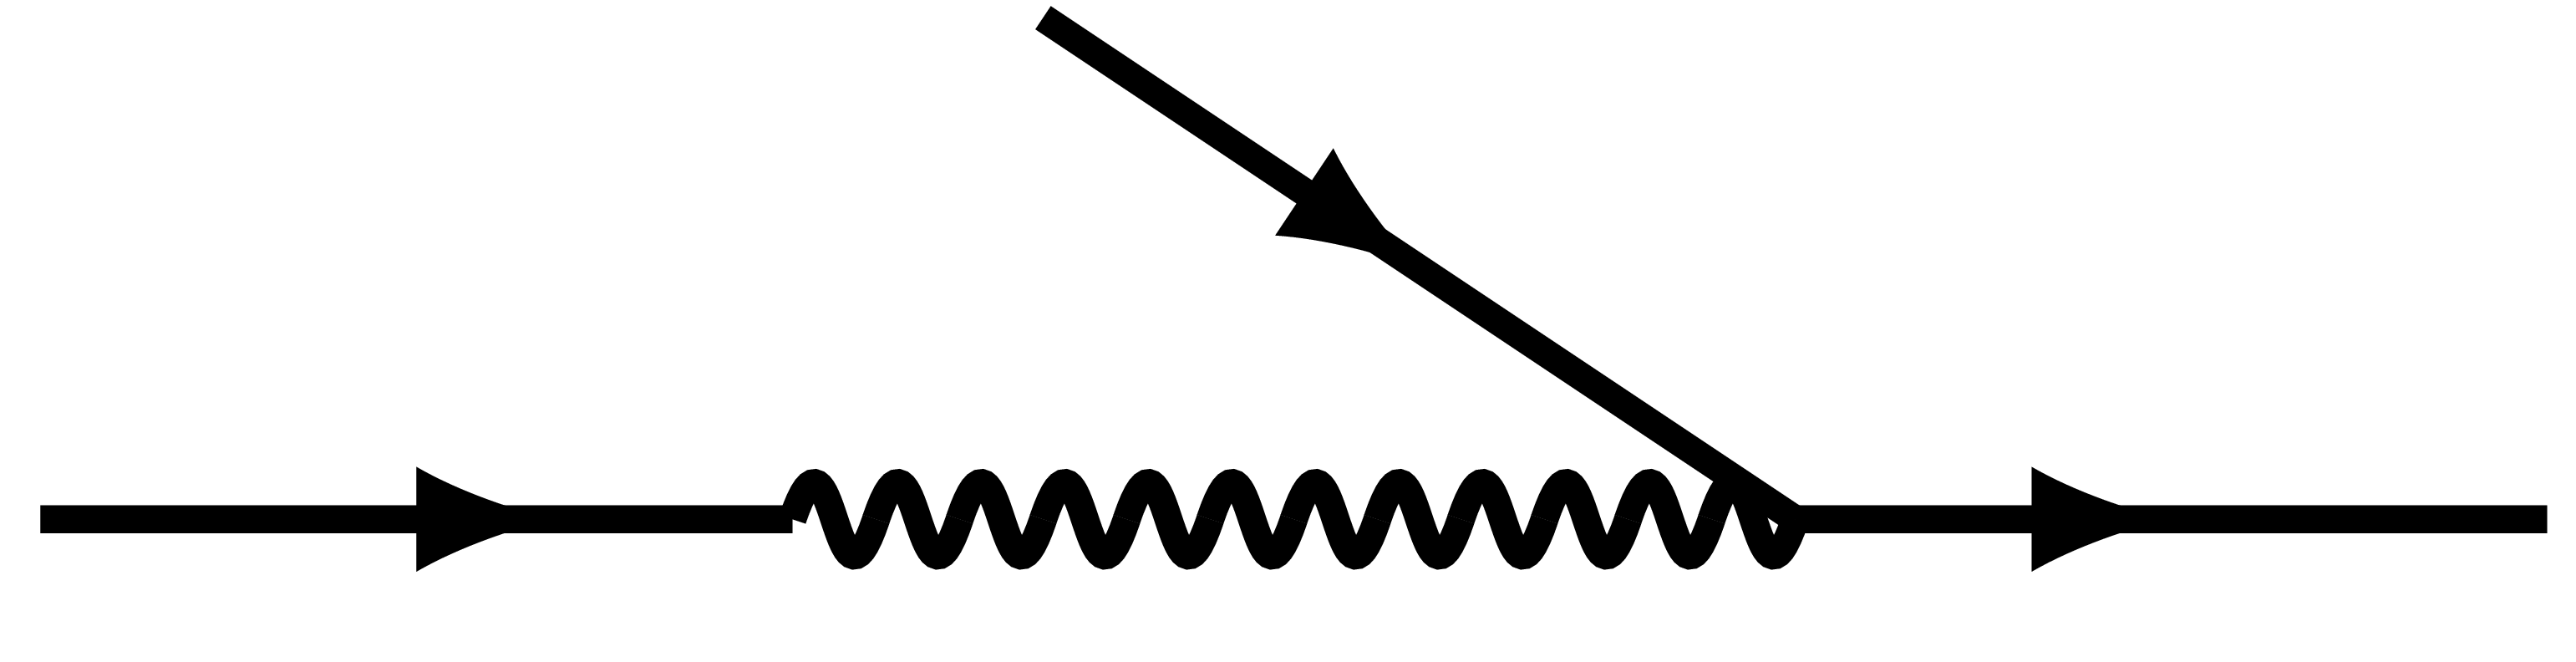
\includegraphics[align=c,width=1.2in]{AB}&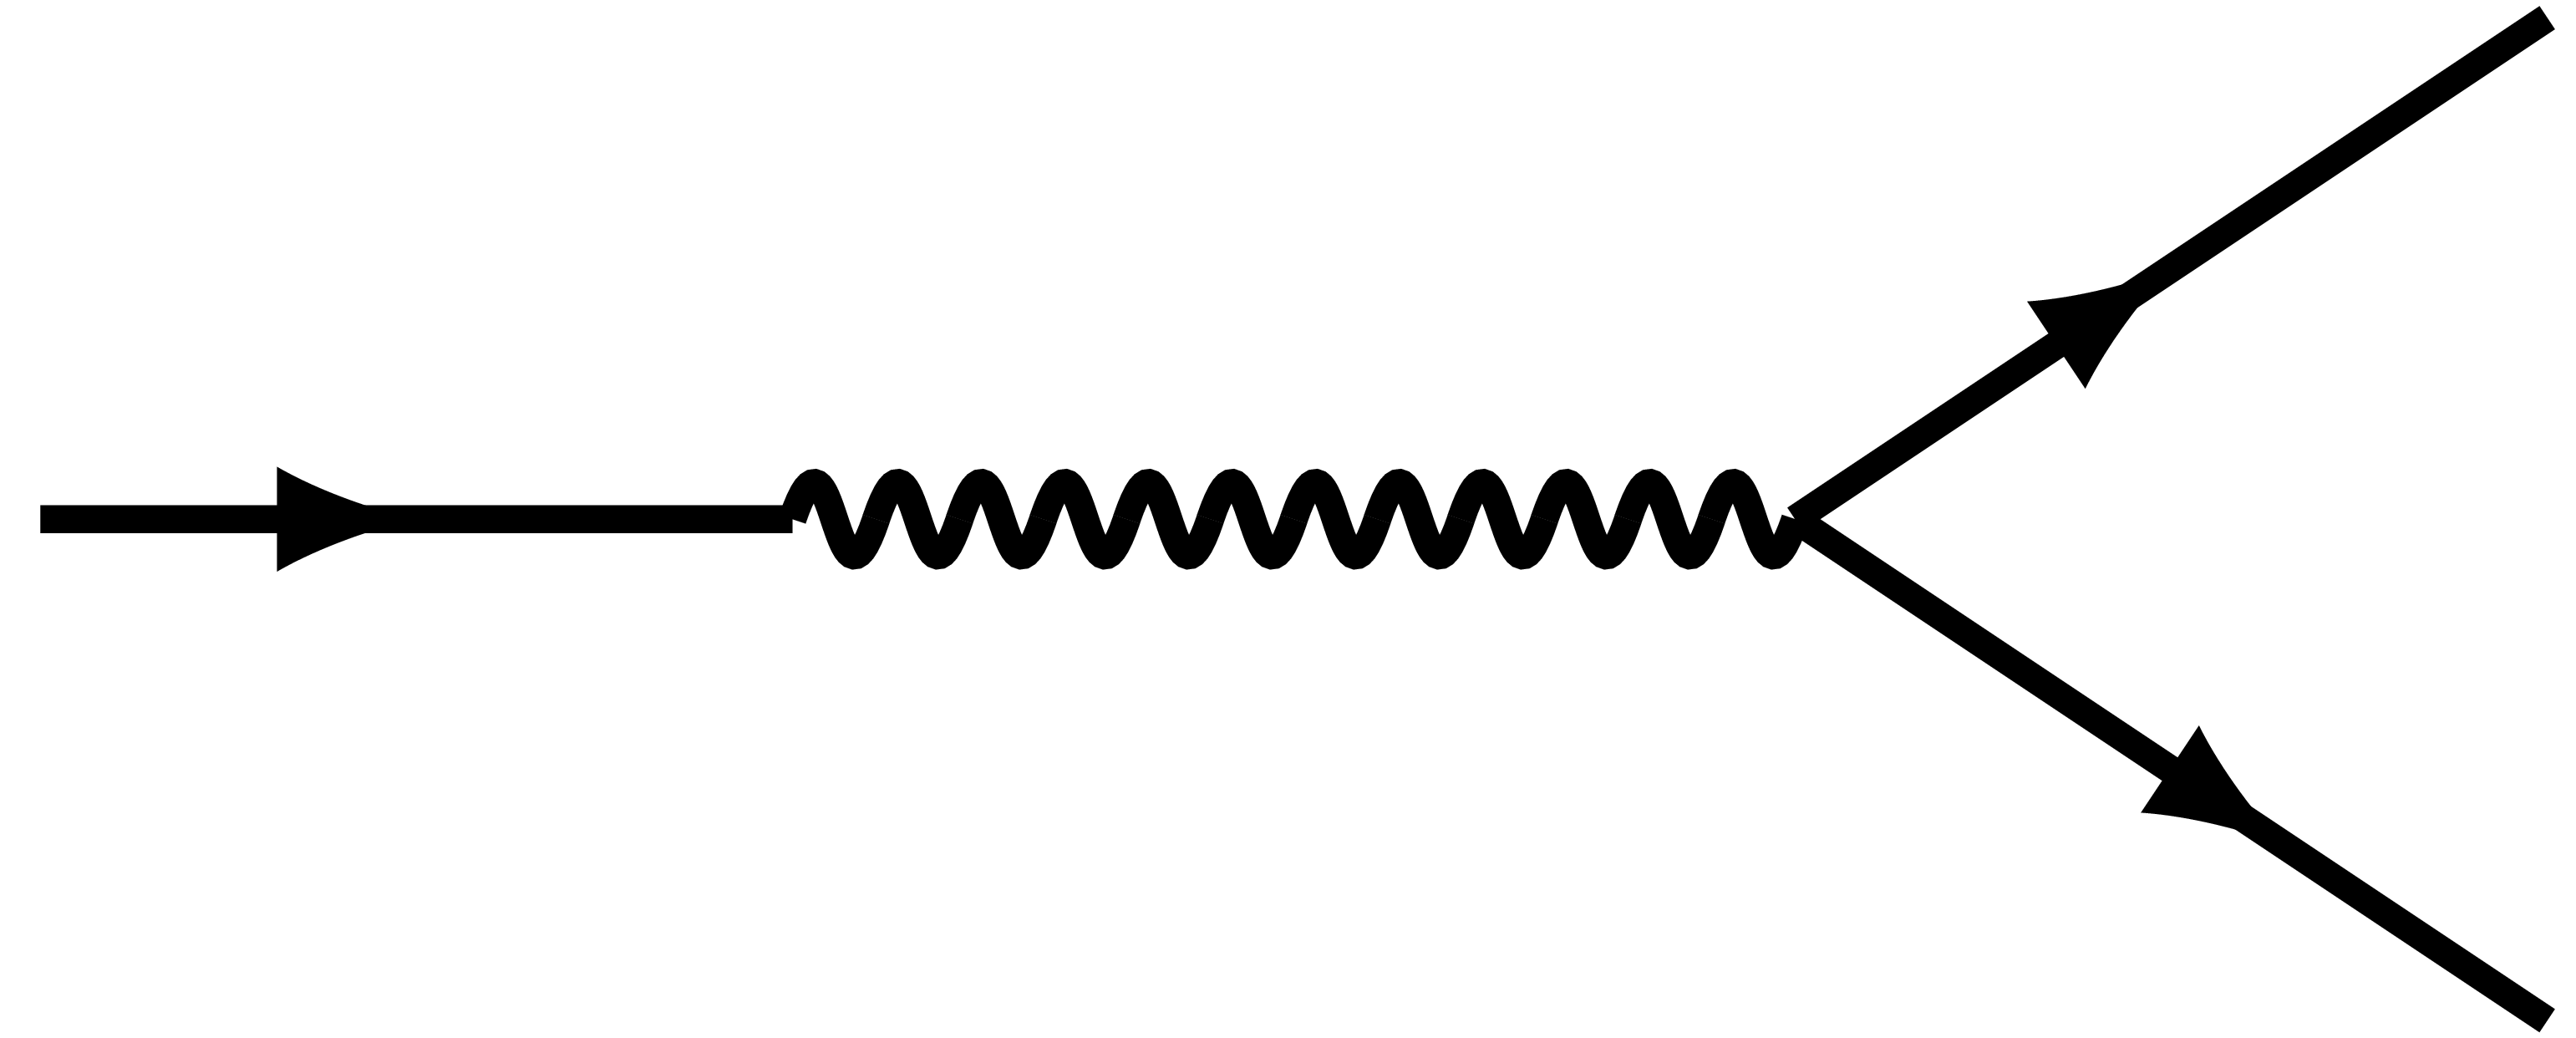
\includegraphics[align=c,width=1.2in]{AC}&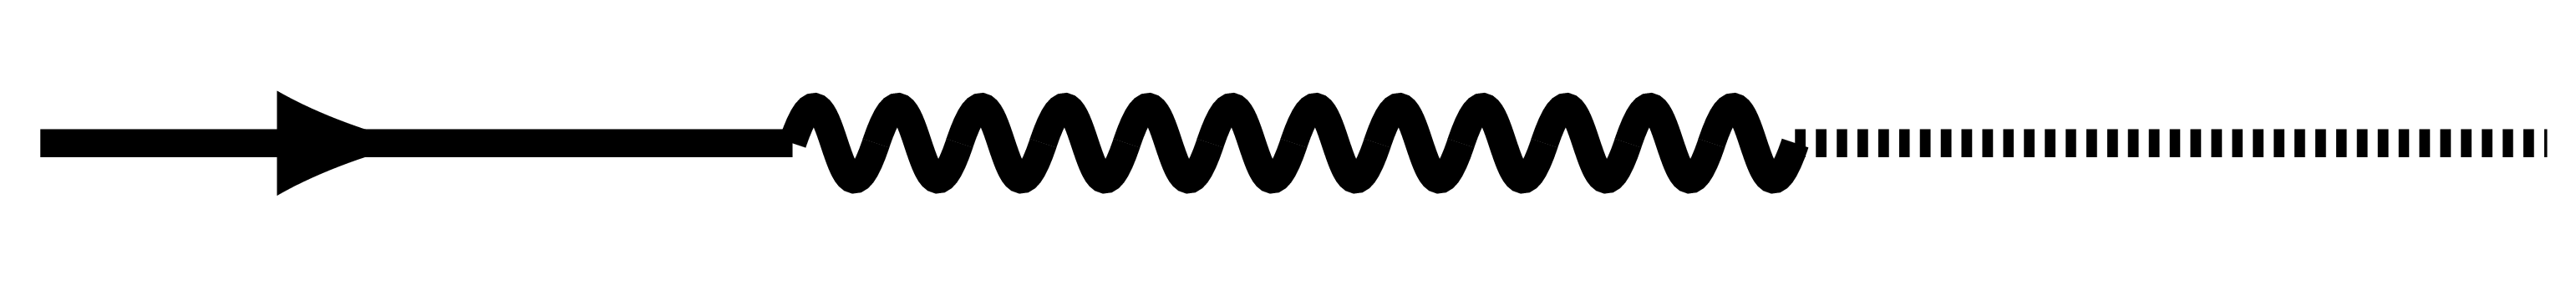
\includegraphics[align=c,width=1.2in]{AD}&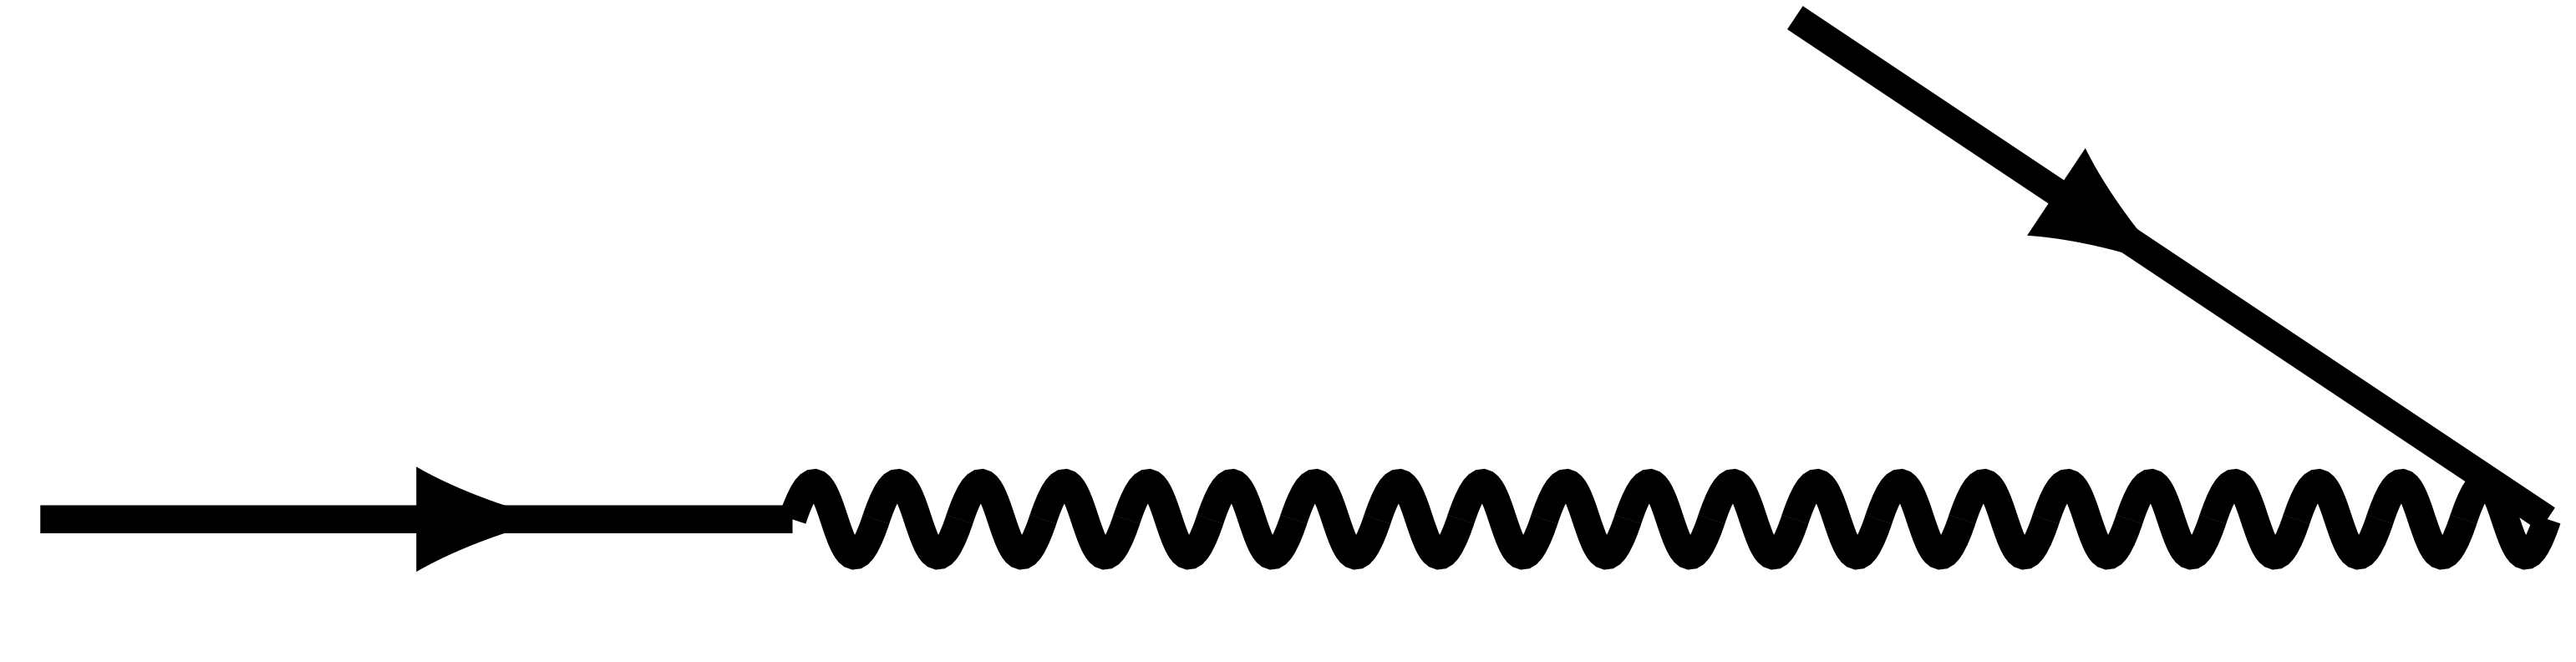
\includegraphics[align=c,width=1.2in]{AE}&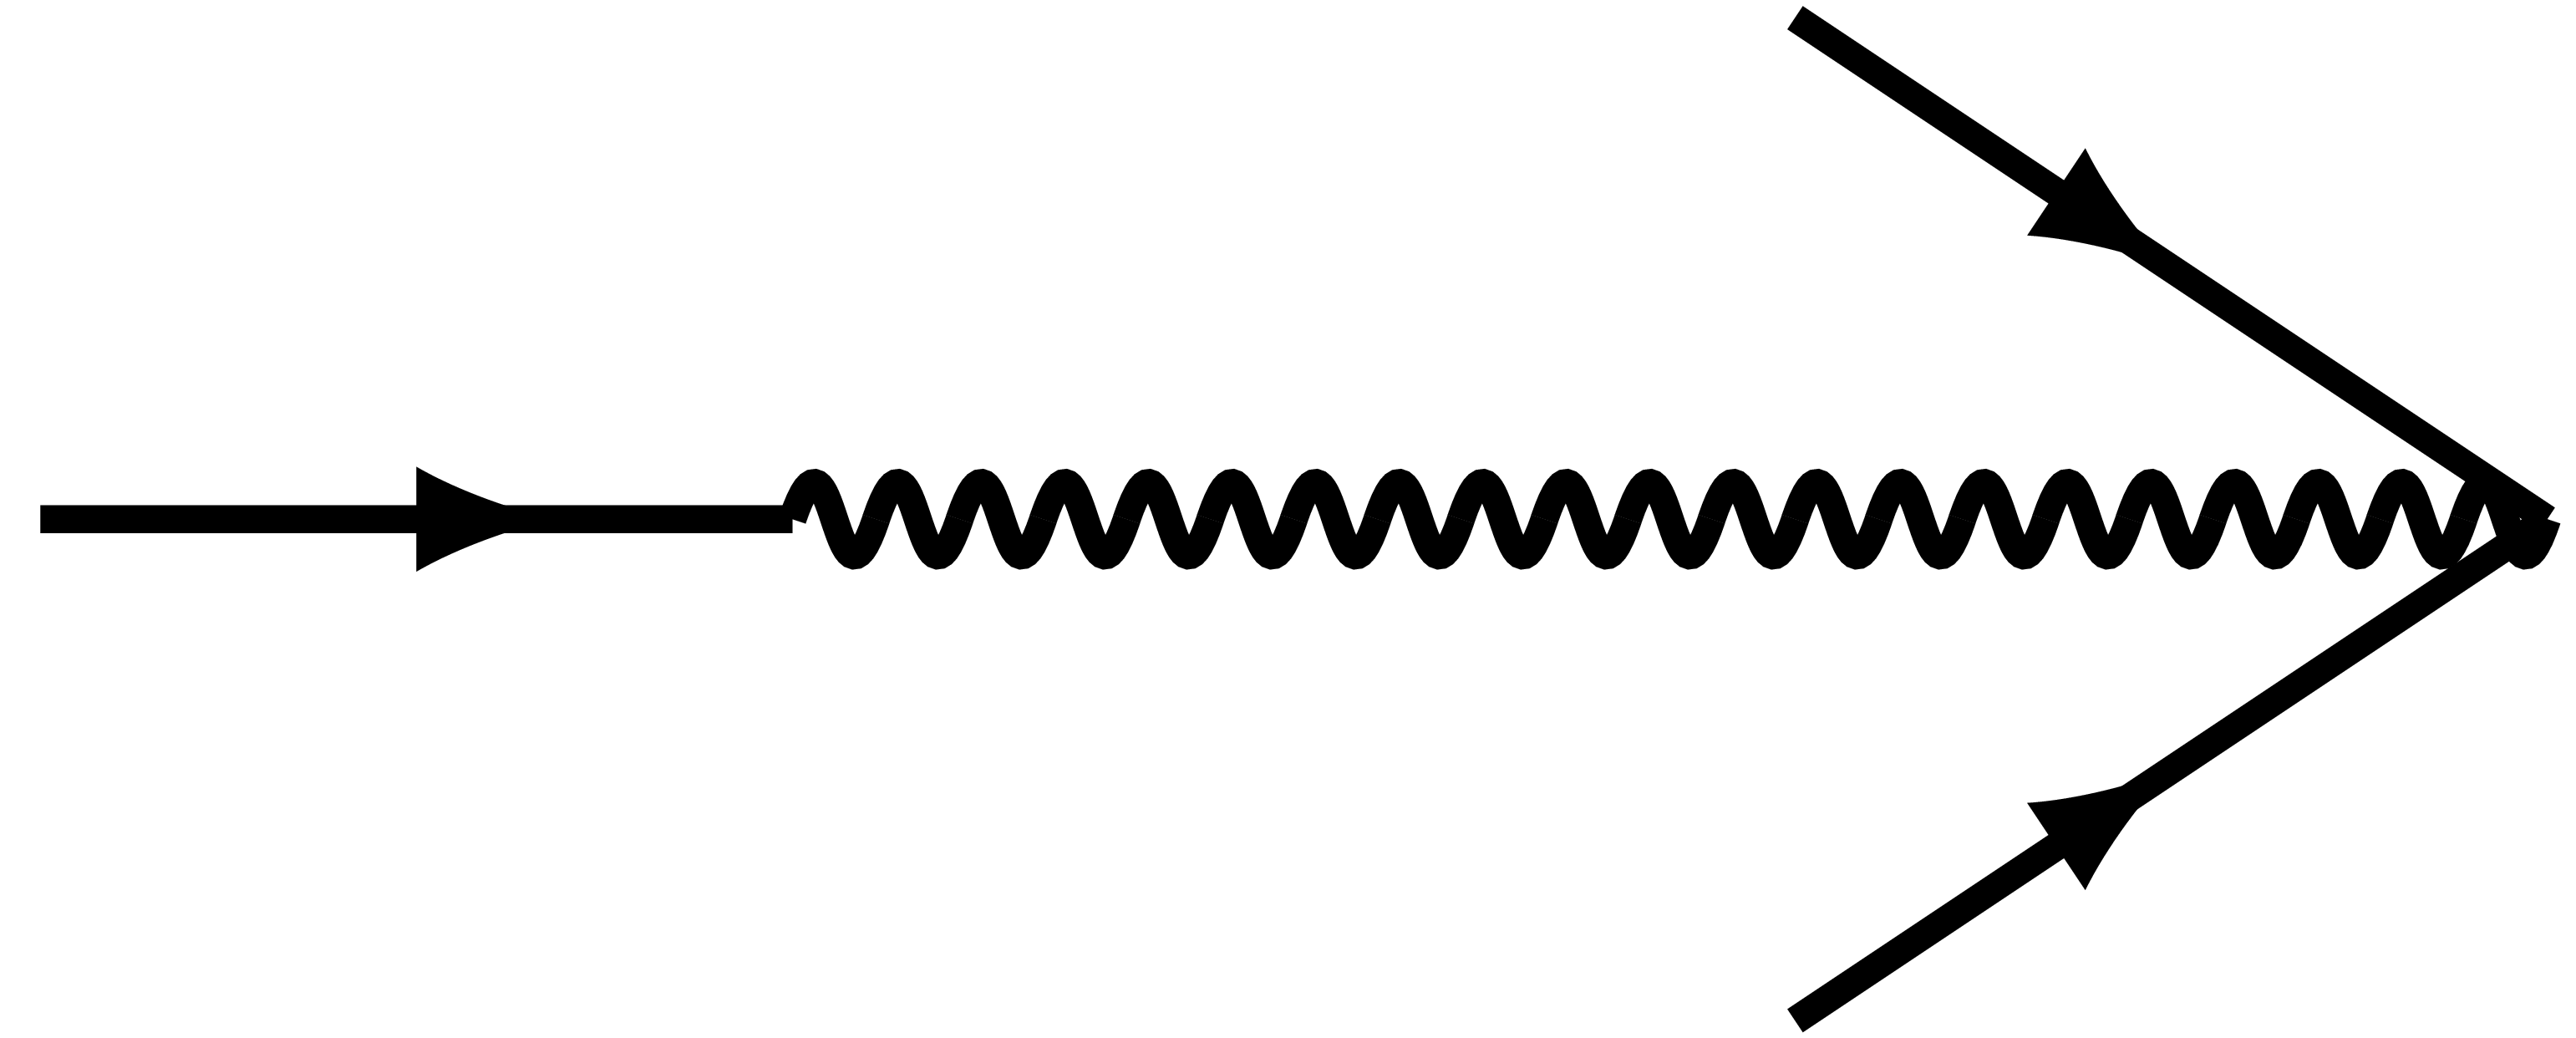
\includegraphics[align=c,width=1.2in]{AF}\\
        $B$ & 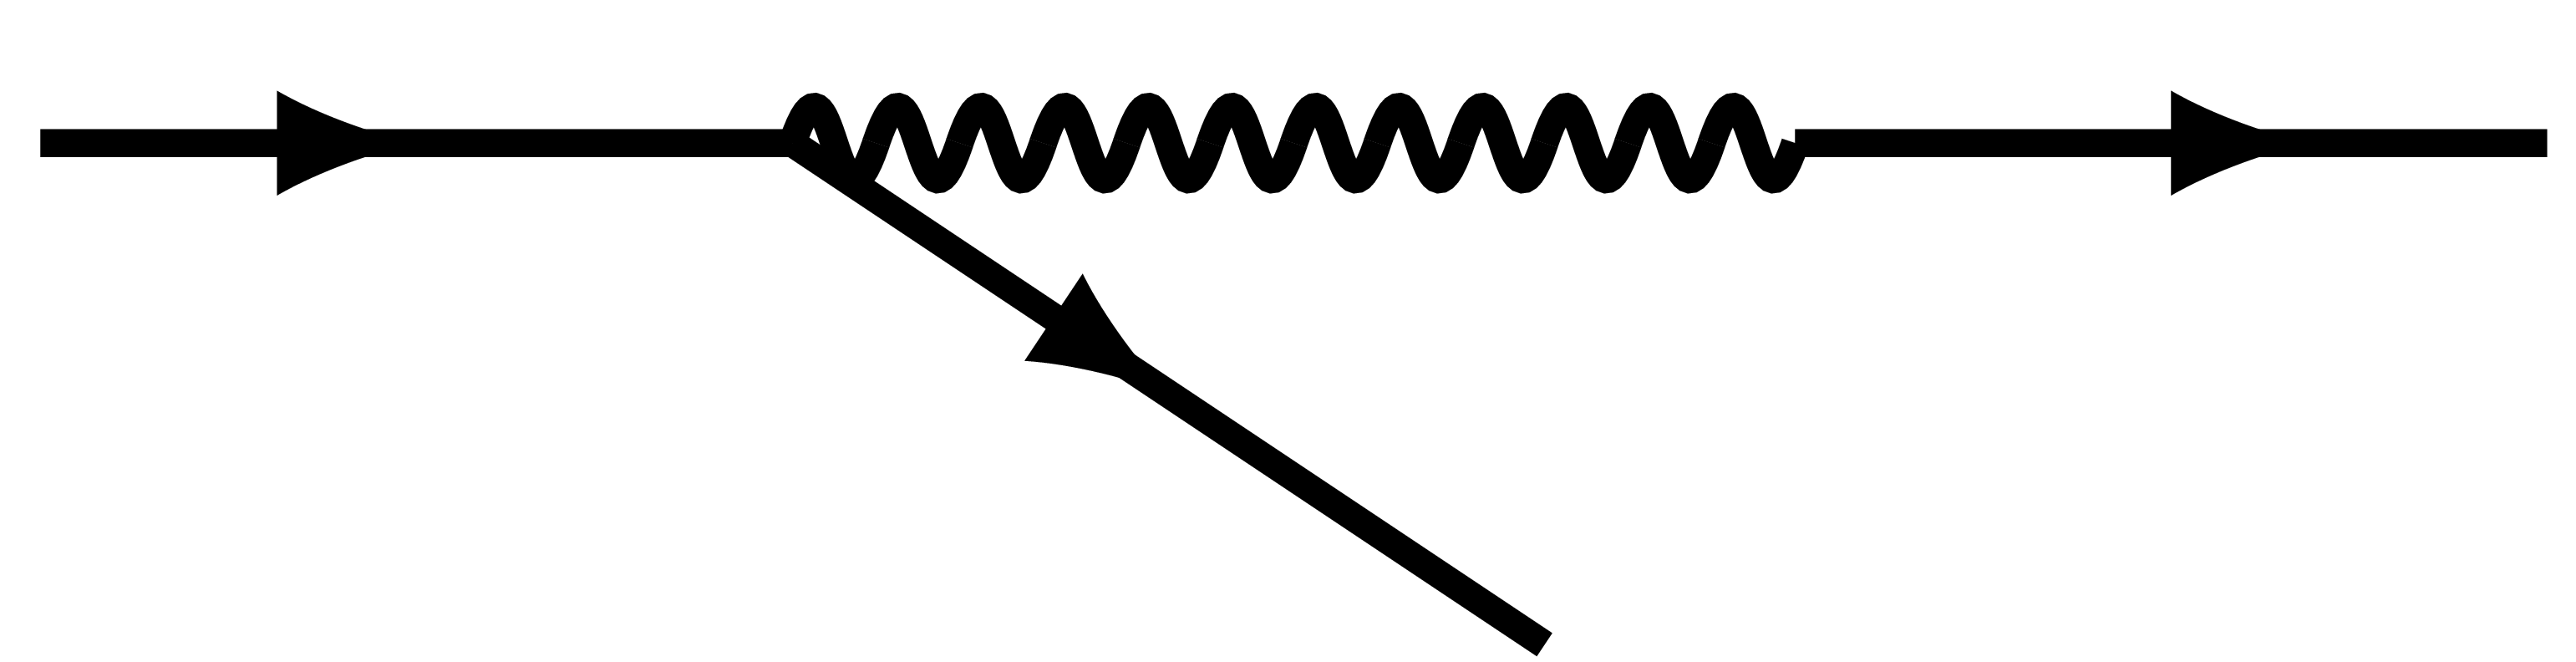
\includegraphics[align=c,width=1.2in]{BA}&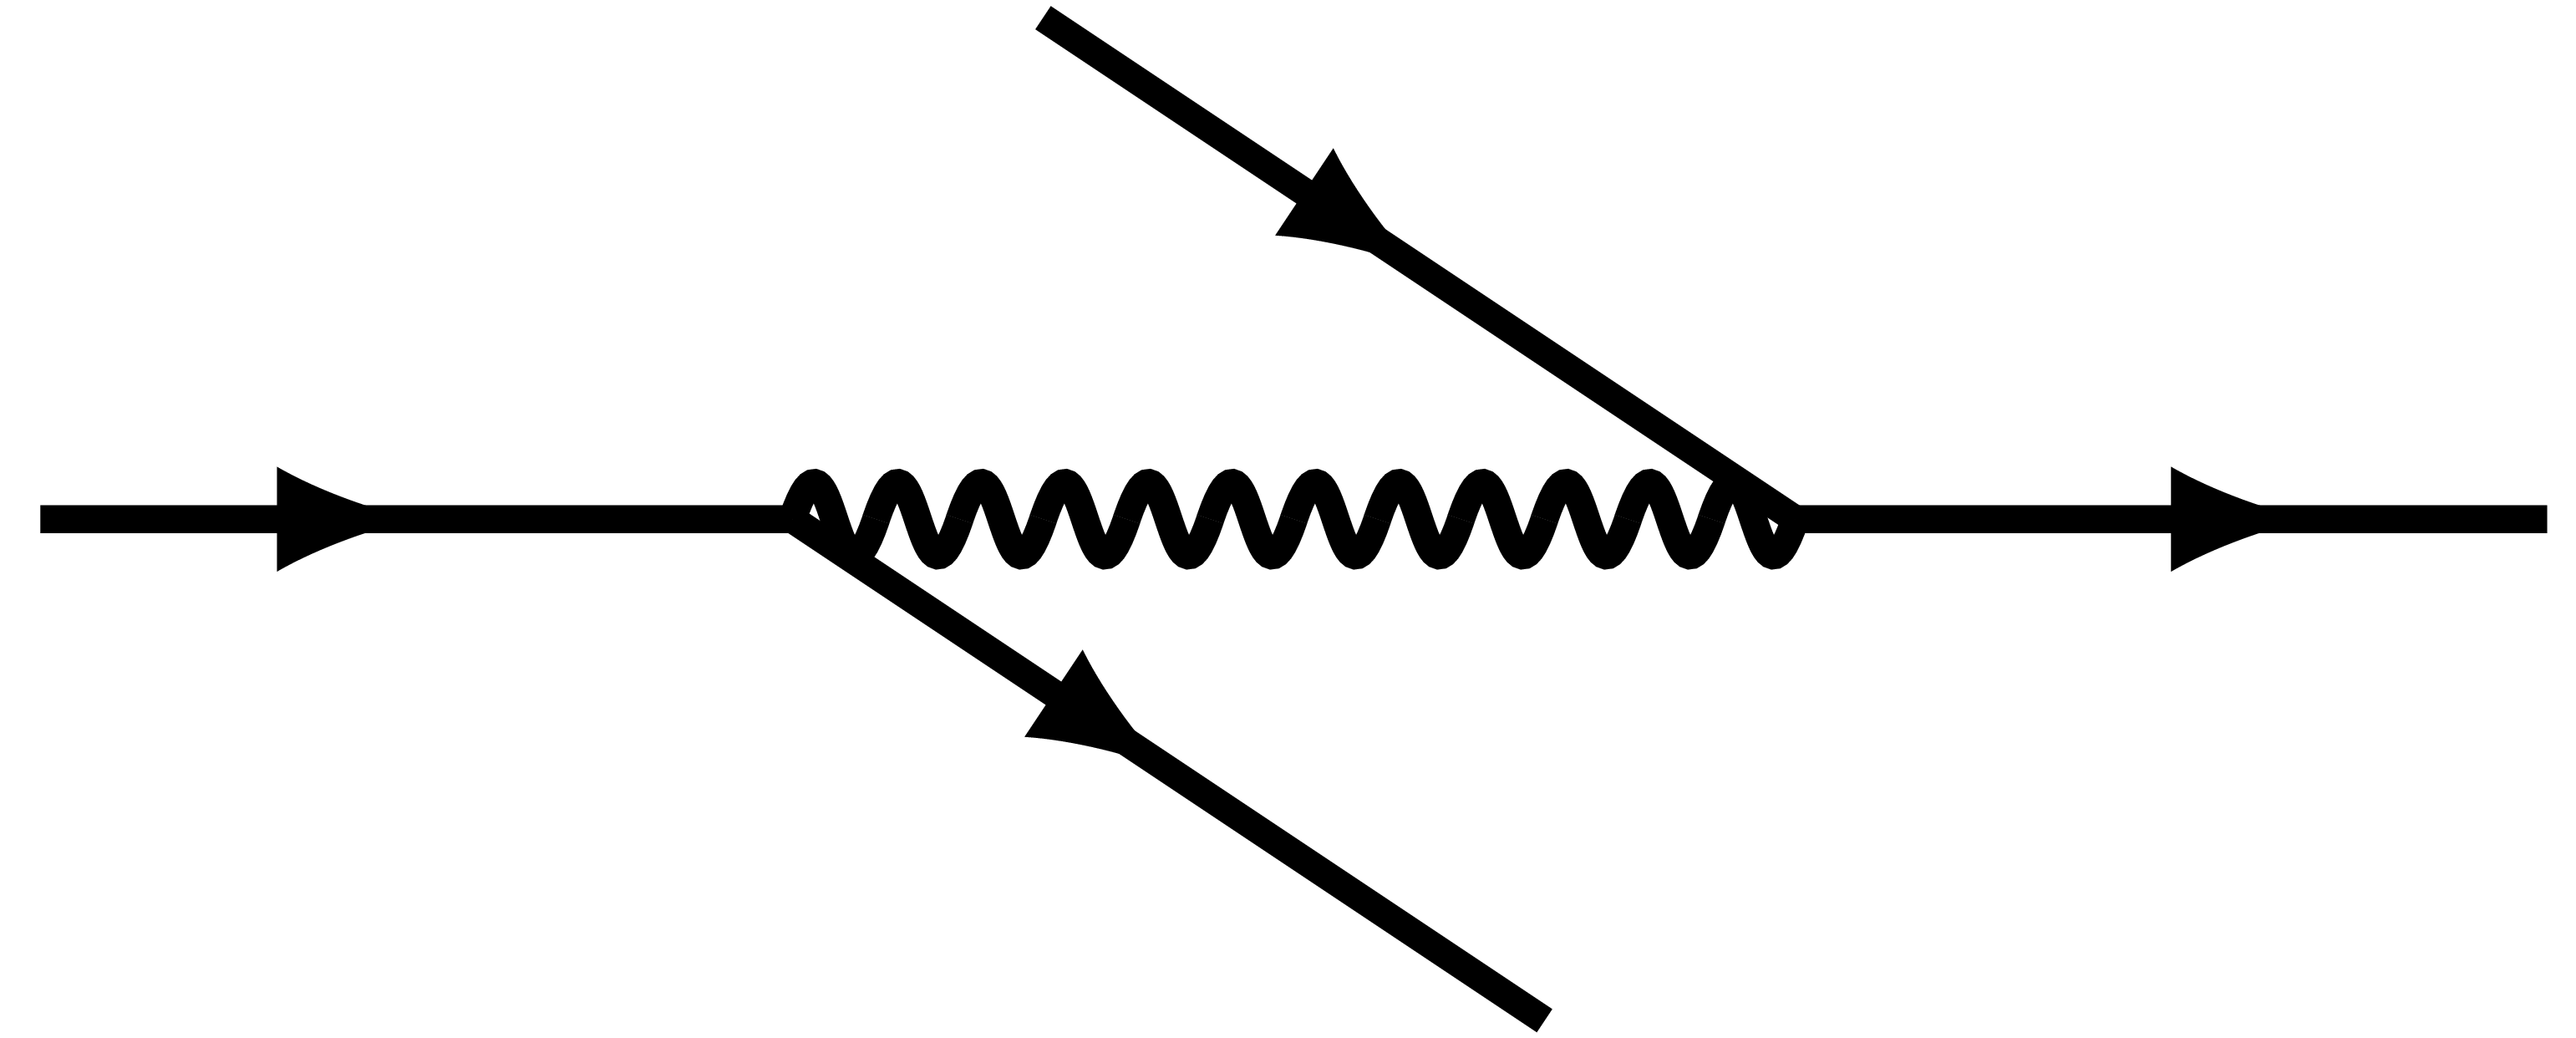
\includegraphics[align=c,width=1.2in]{BB}&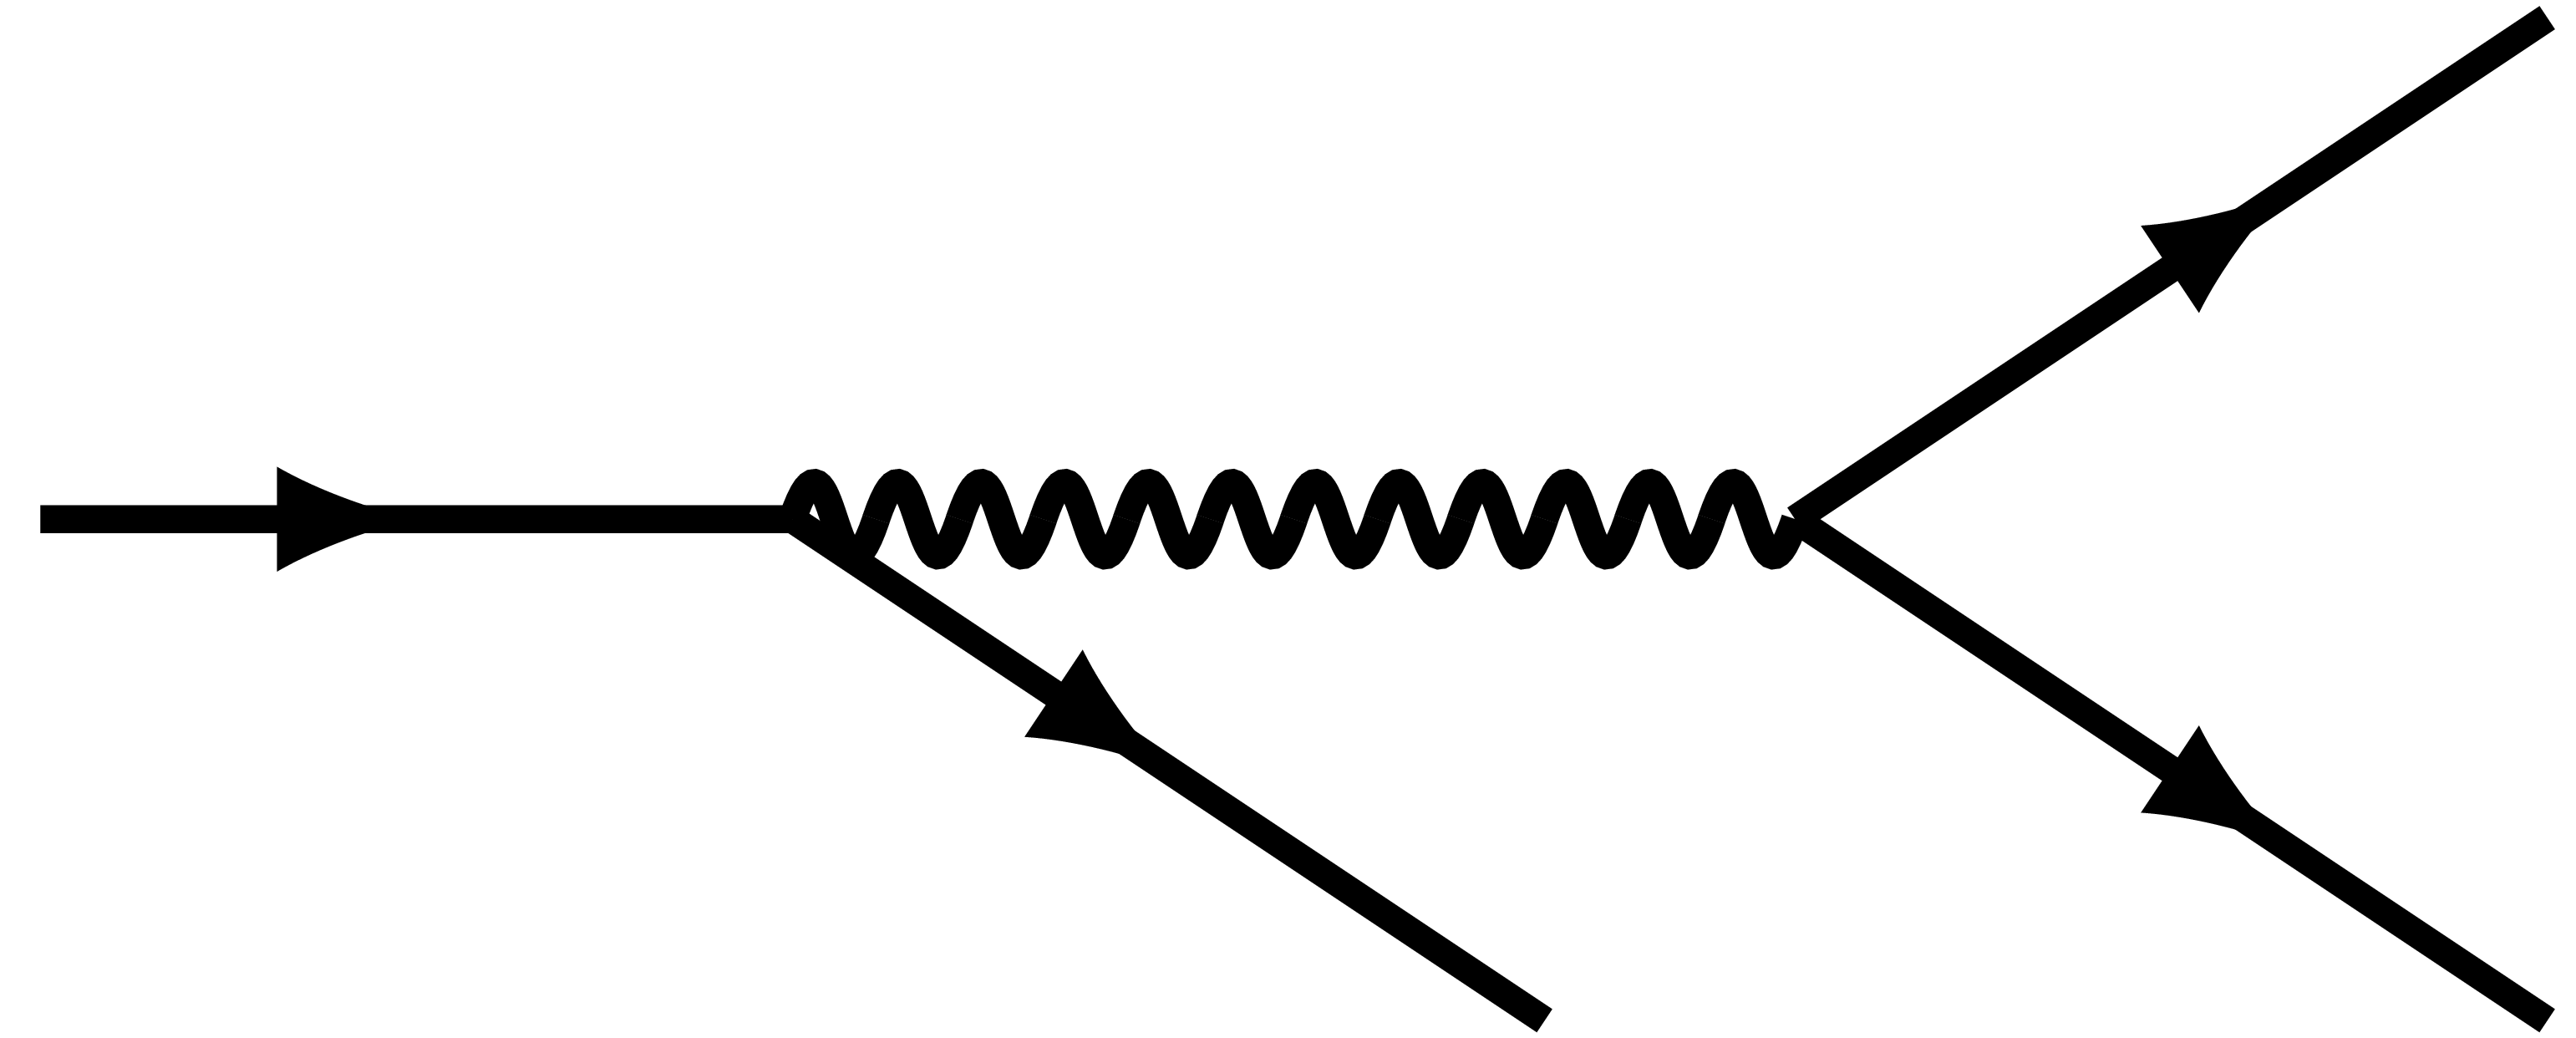
\includegraphics[align=c,width=1.2in]{BC}&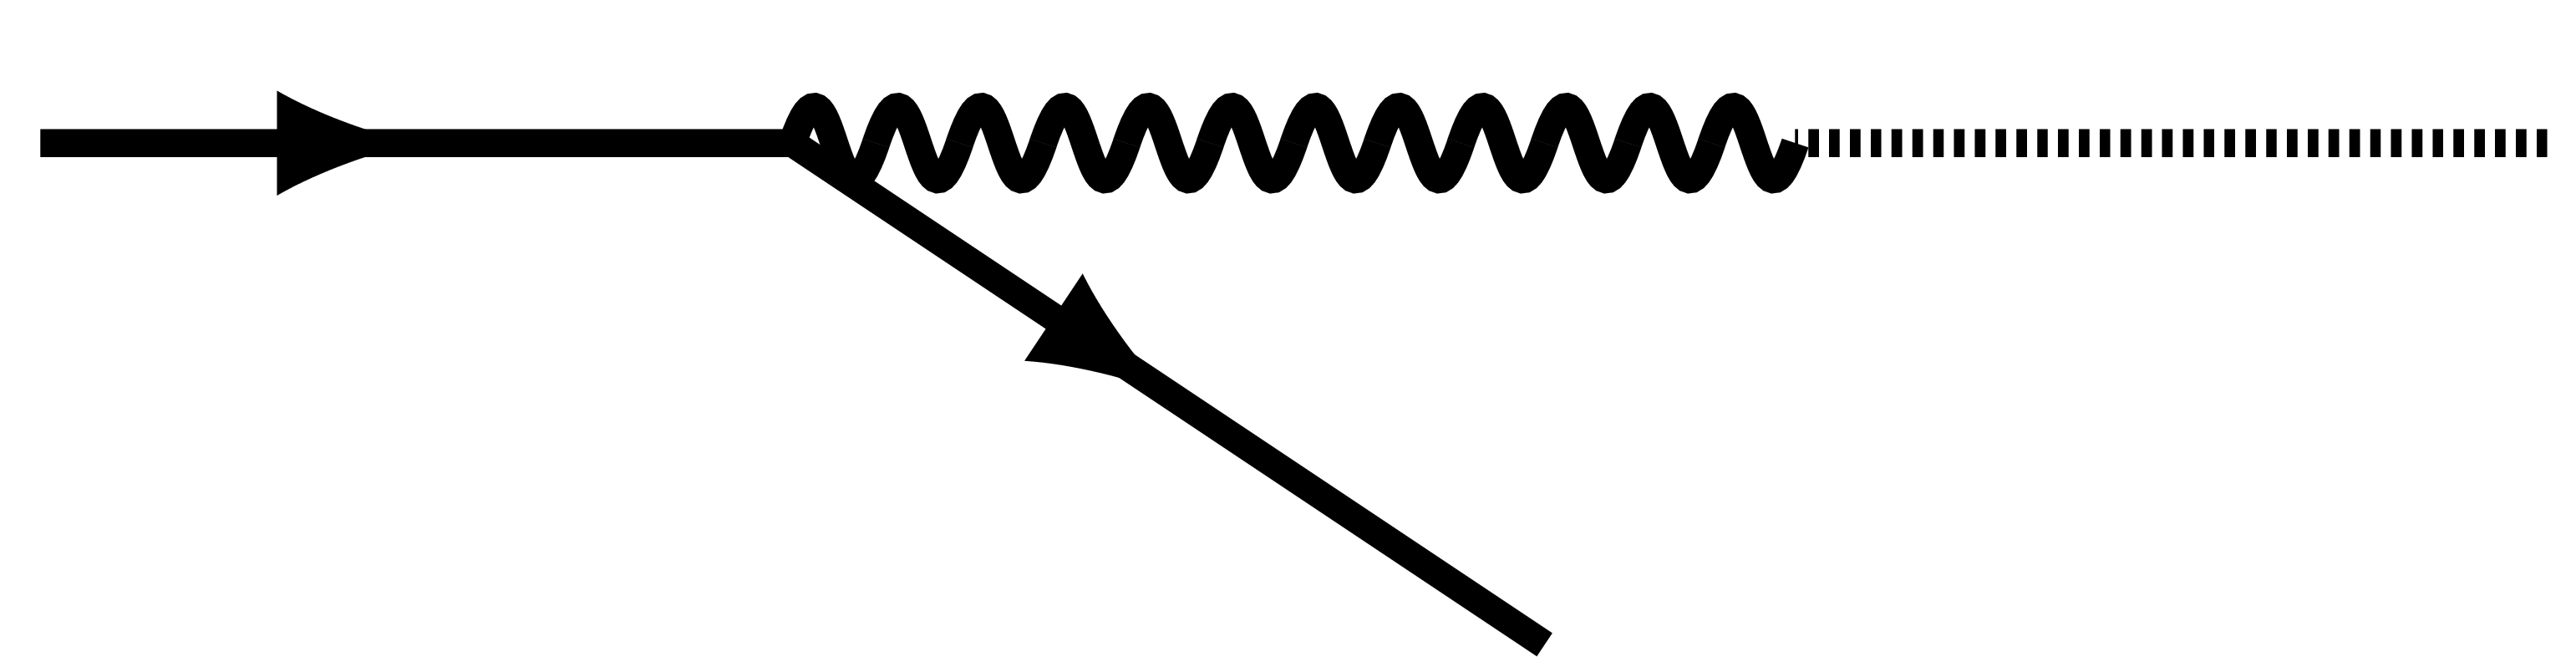
\includegraphics[align=c,width=1.2in]{BD}&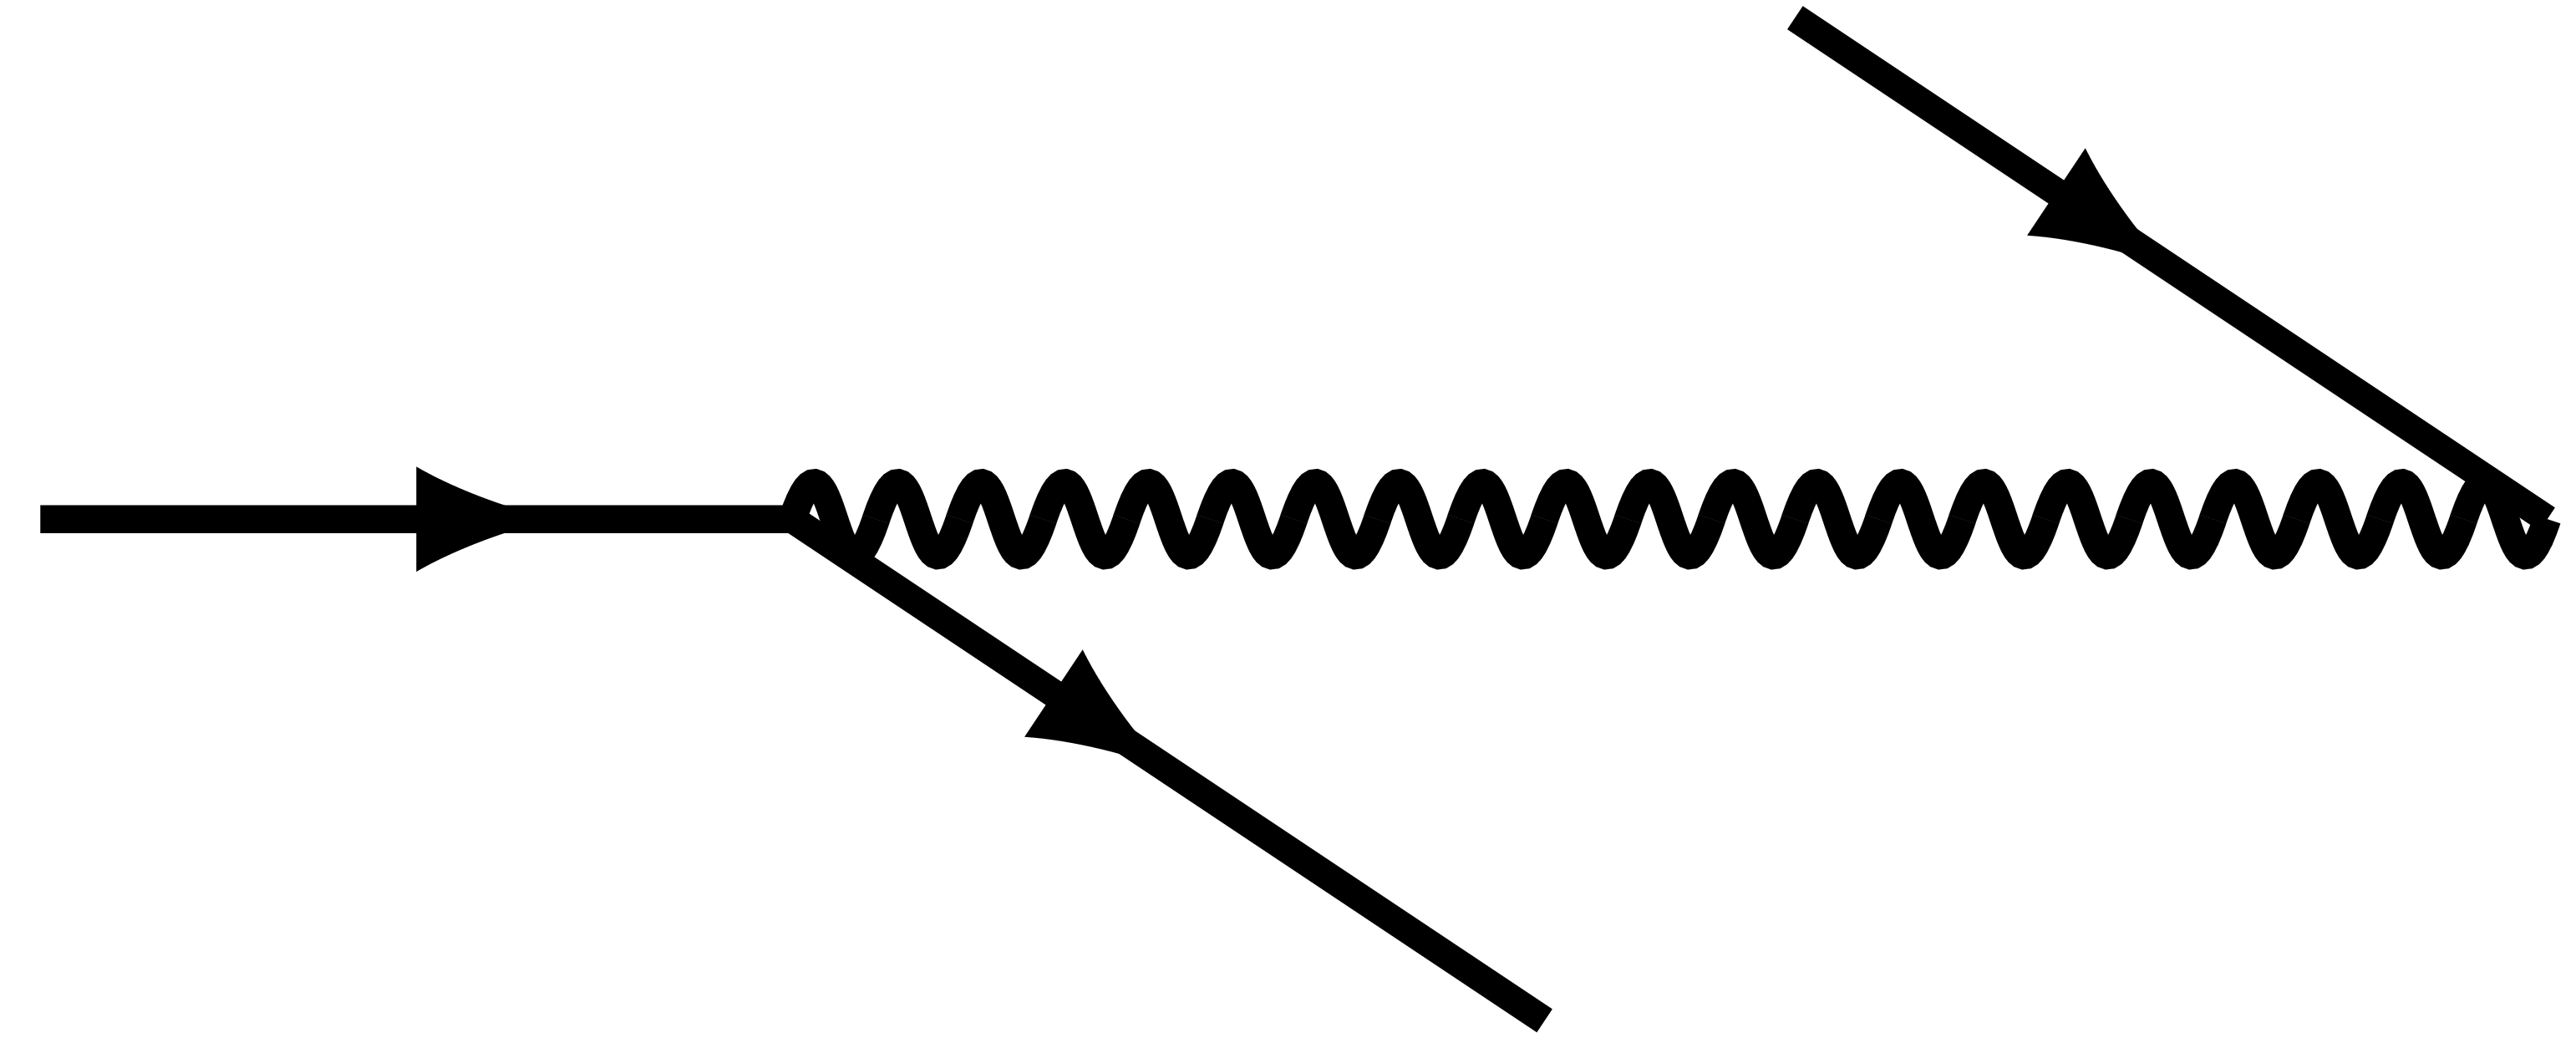
\includegraphics[align=c,width=1.2in]{BE}&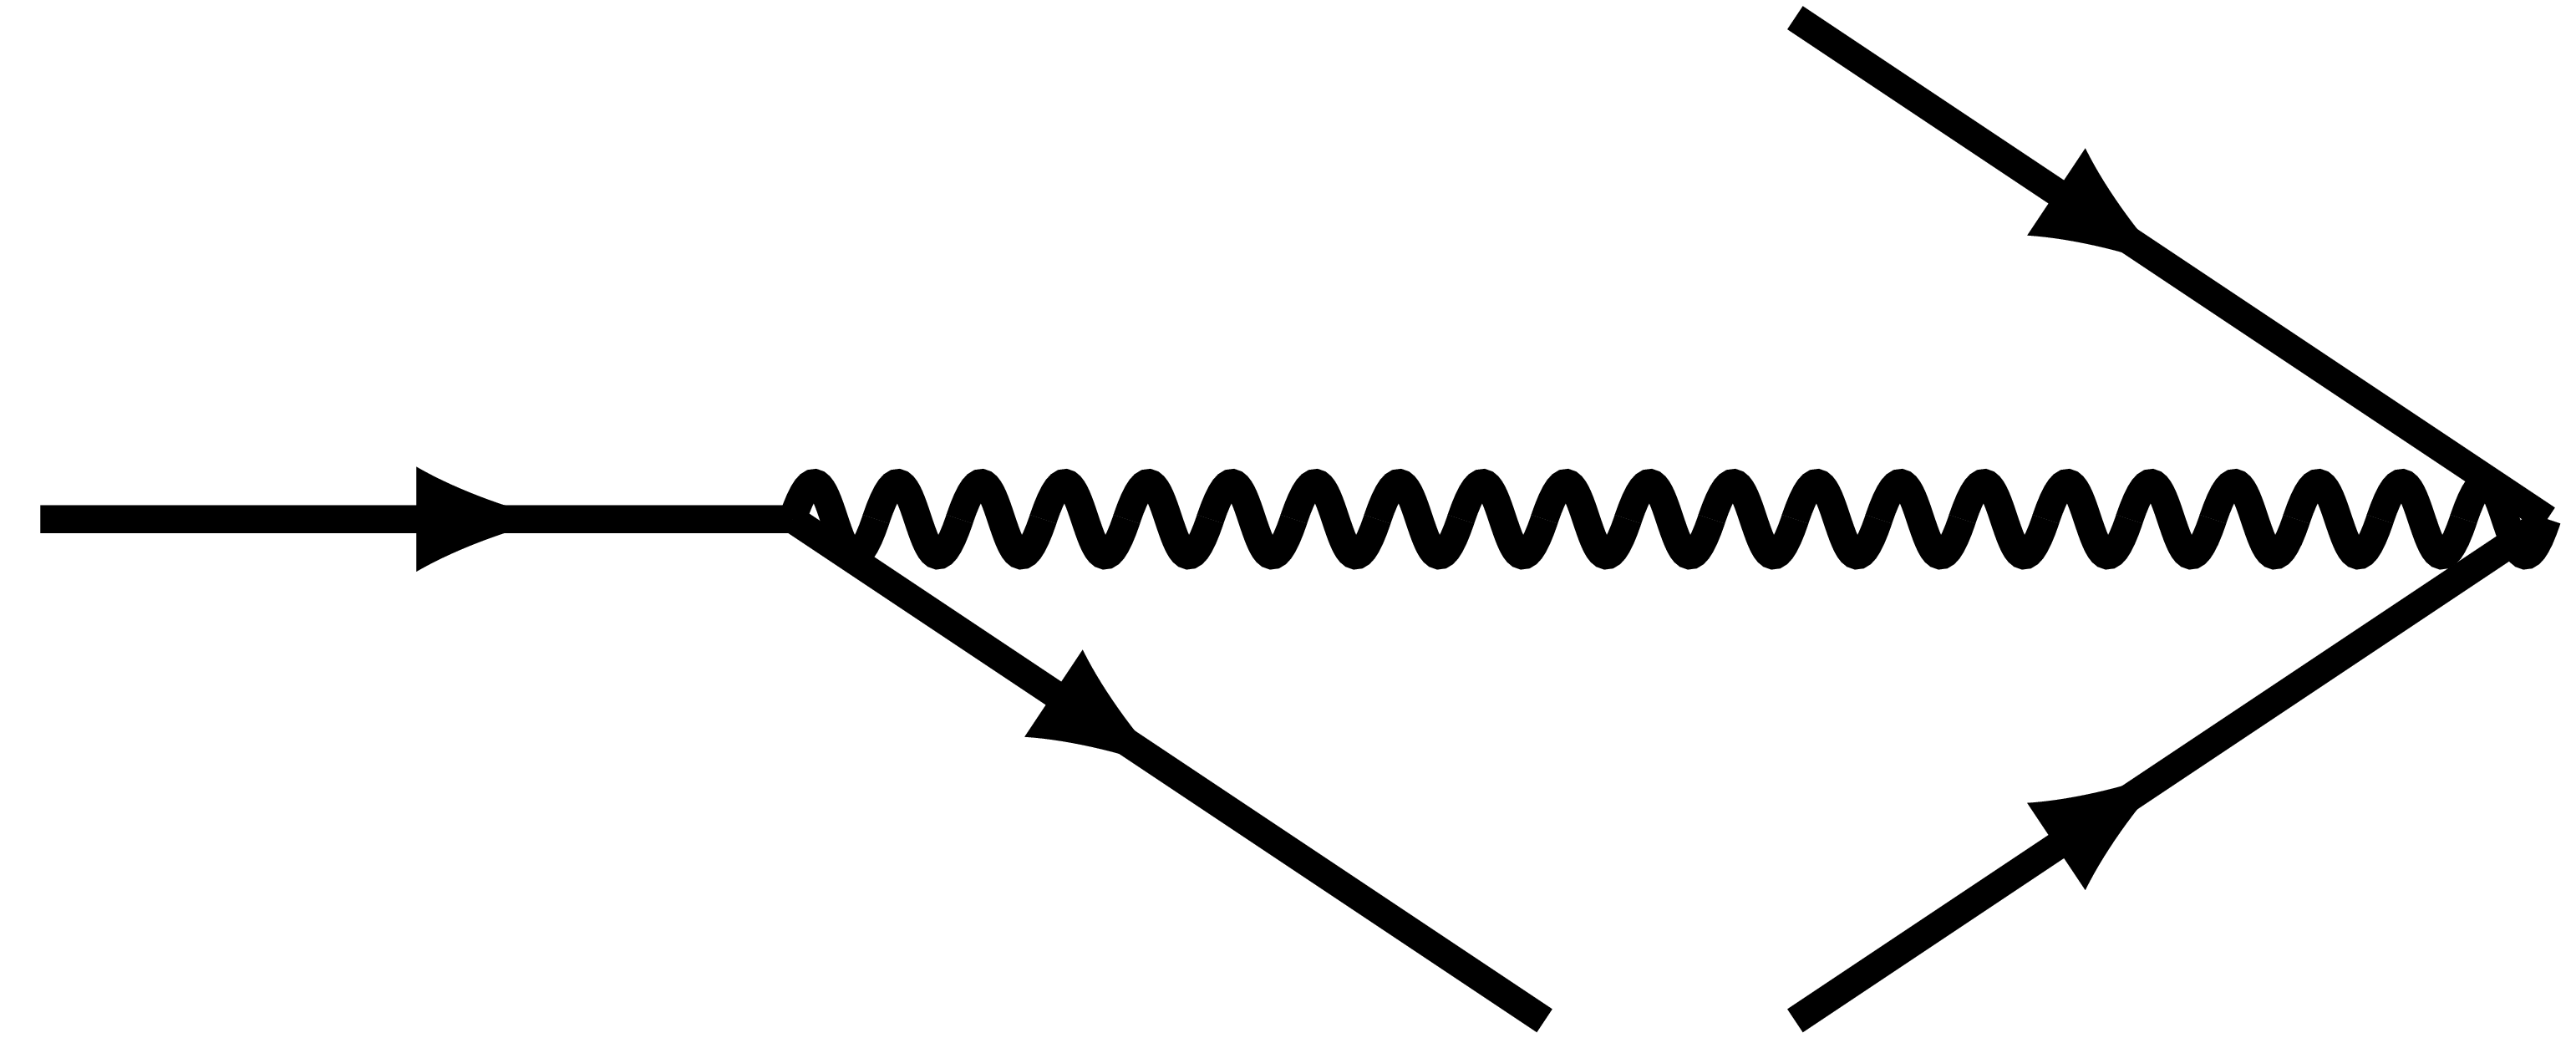
\includegraphics[align=c,width=1.2in]{BF}\\
        $C$ & 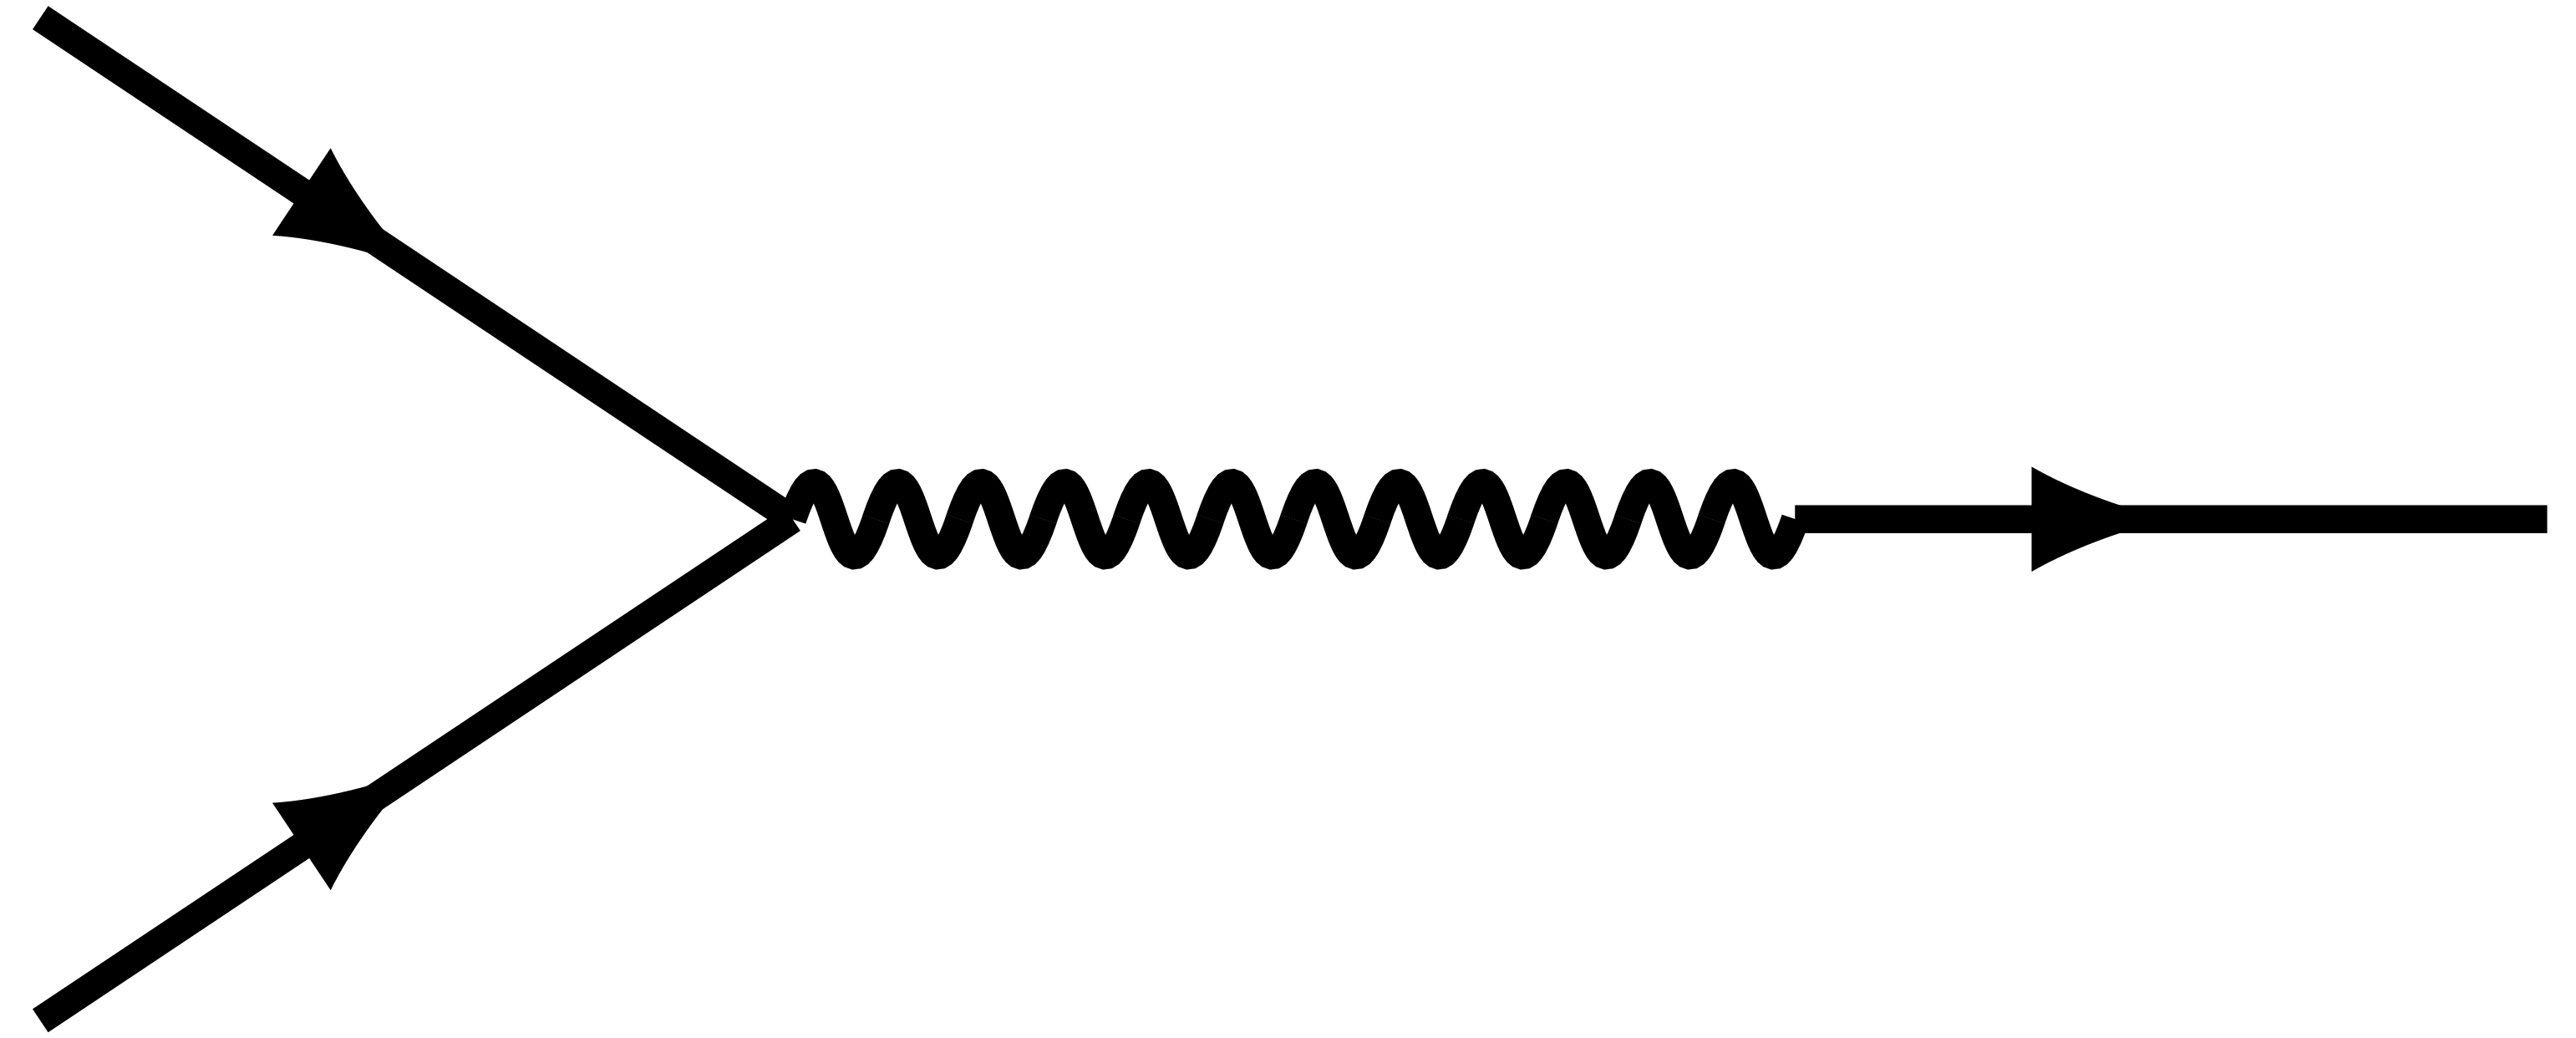
\includegraphics[align=c,width=1.2in]{CA}&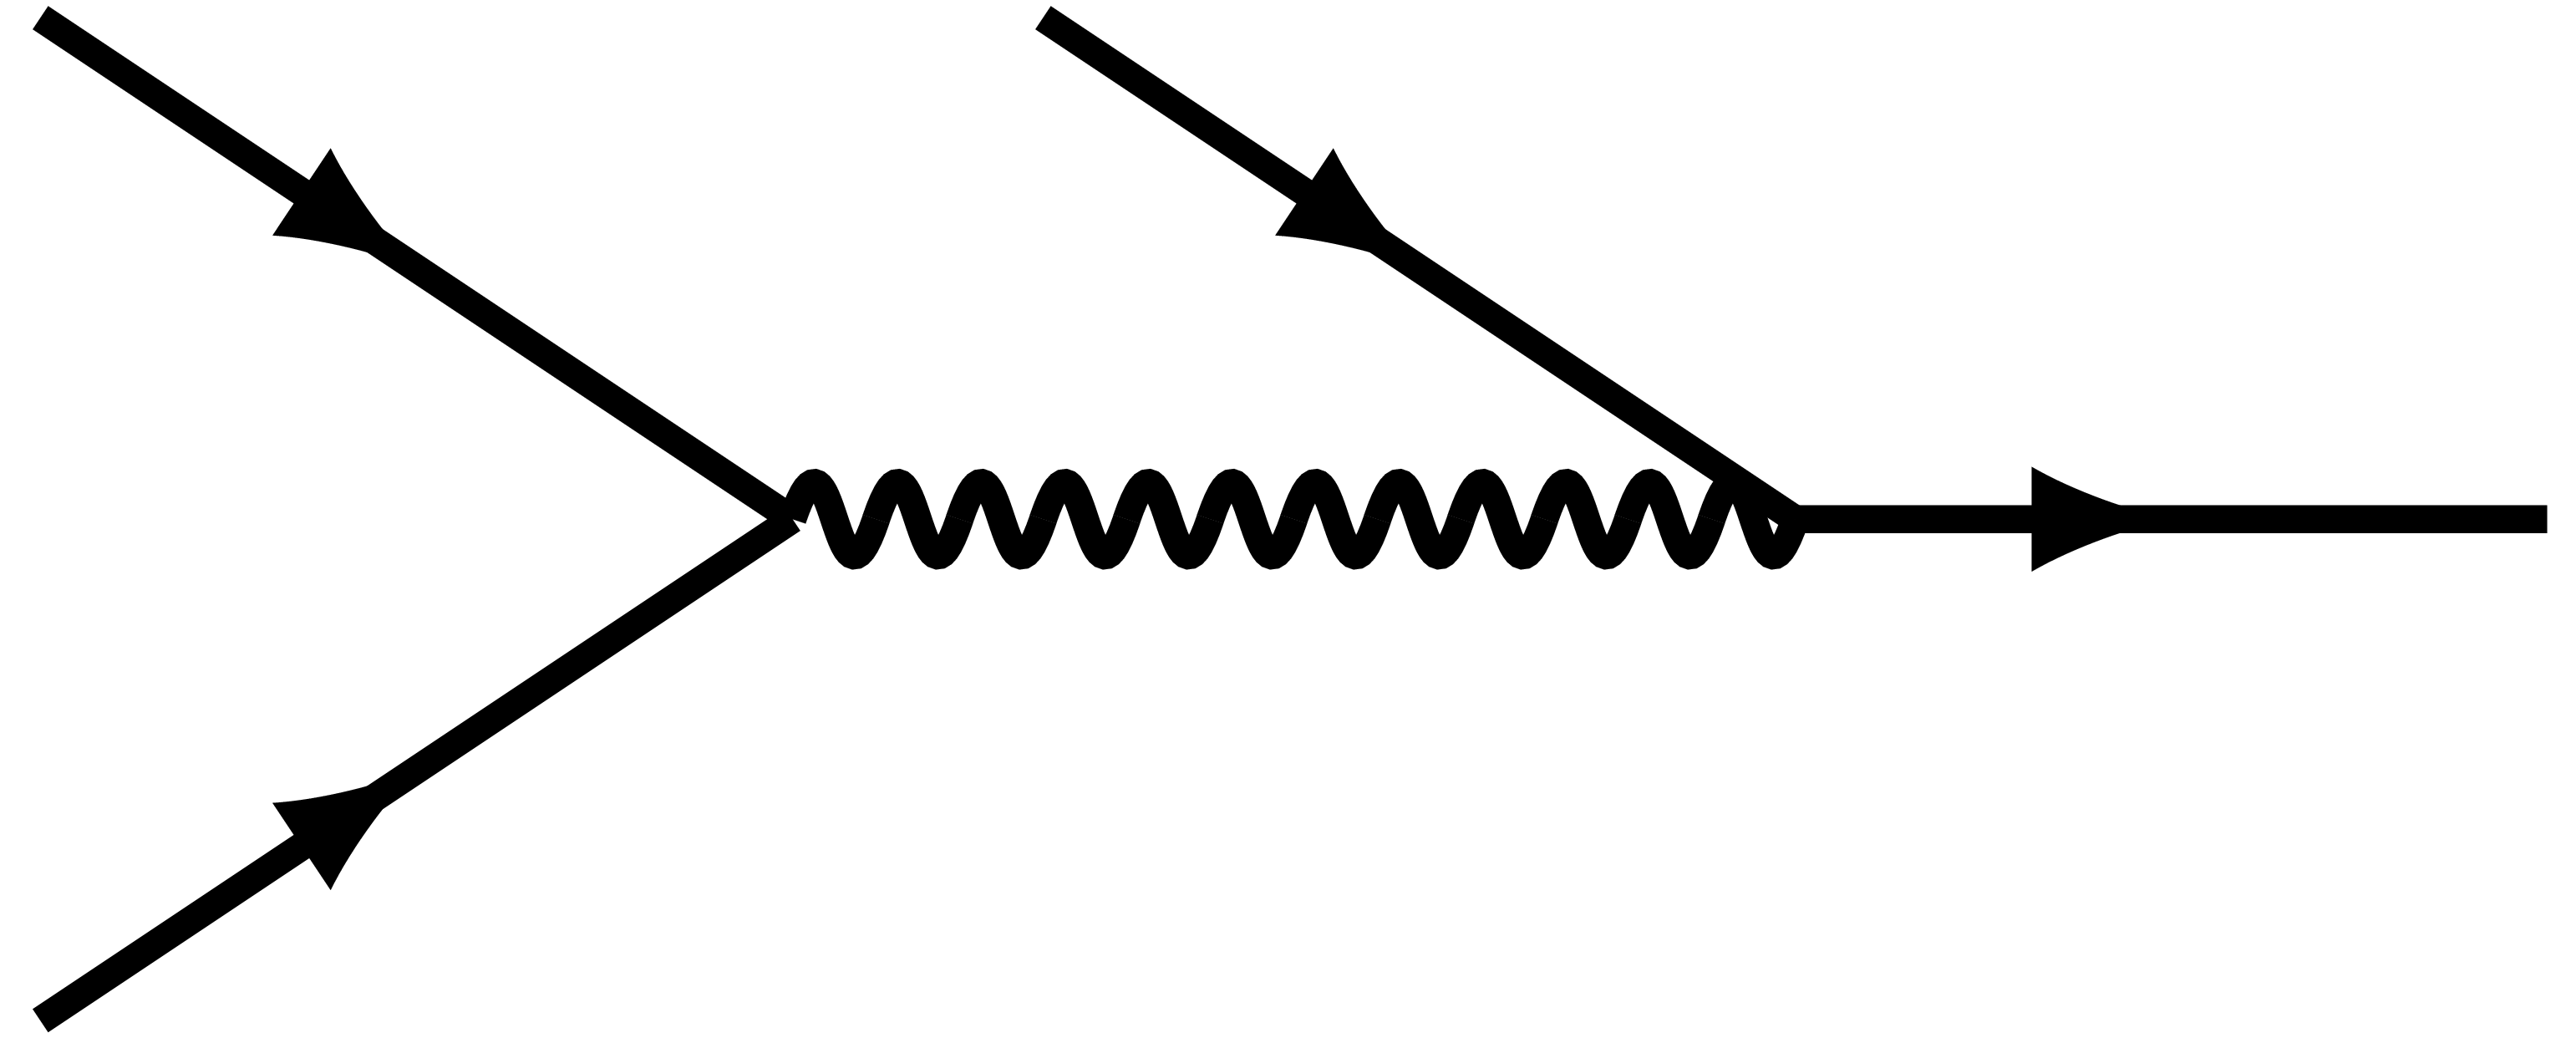
\includegraphics[align=c,width=1.2in]{CB}&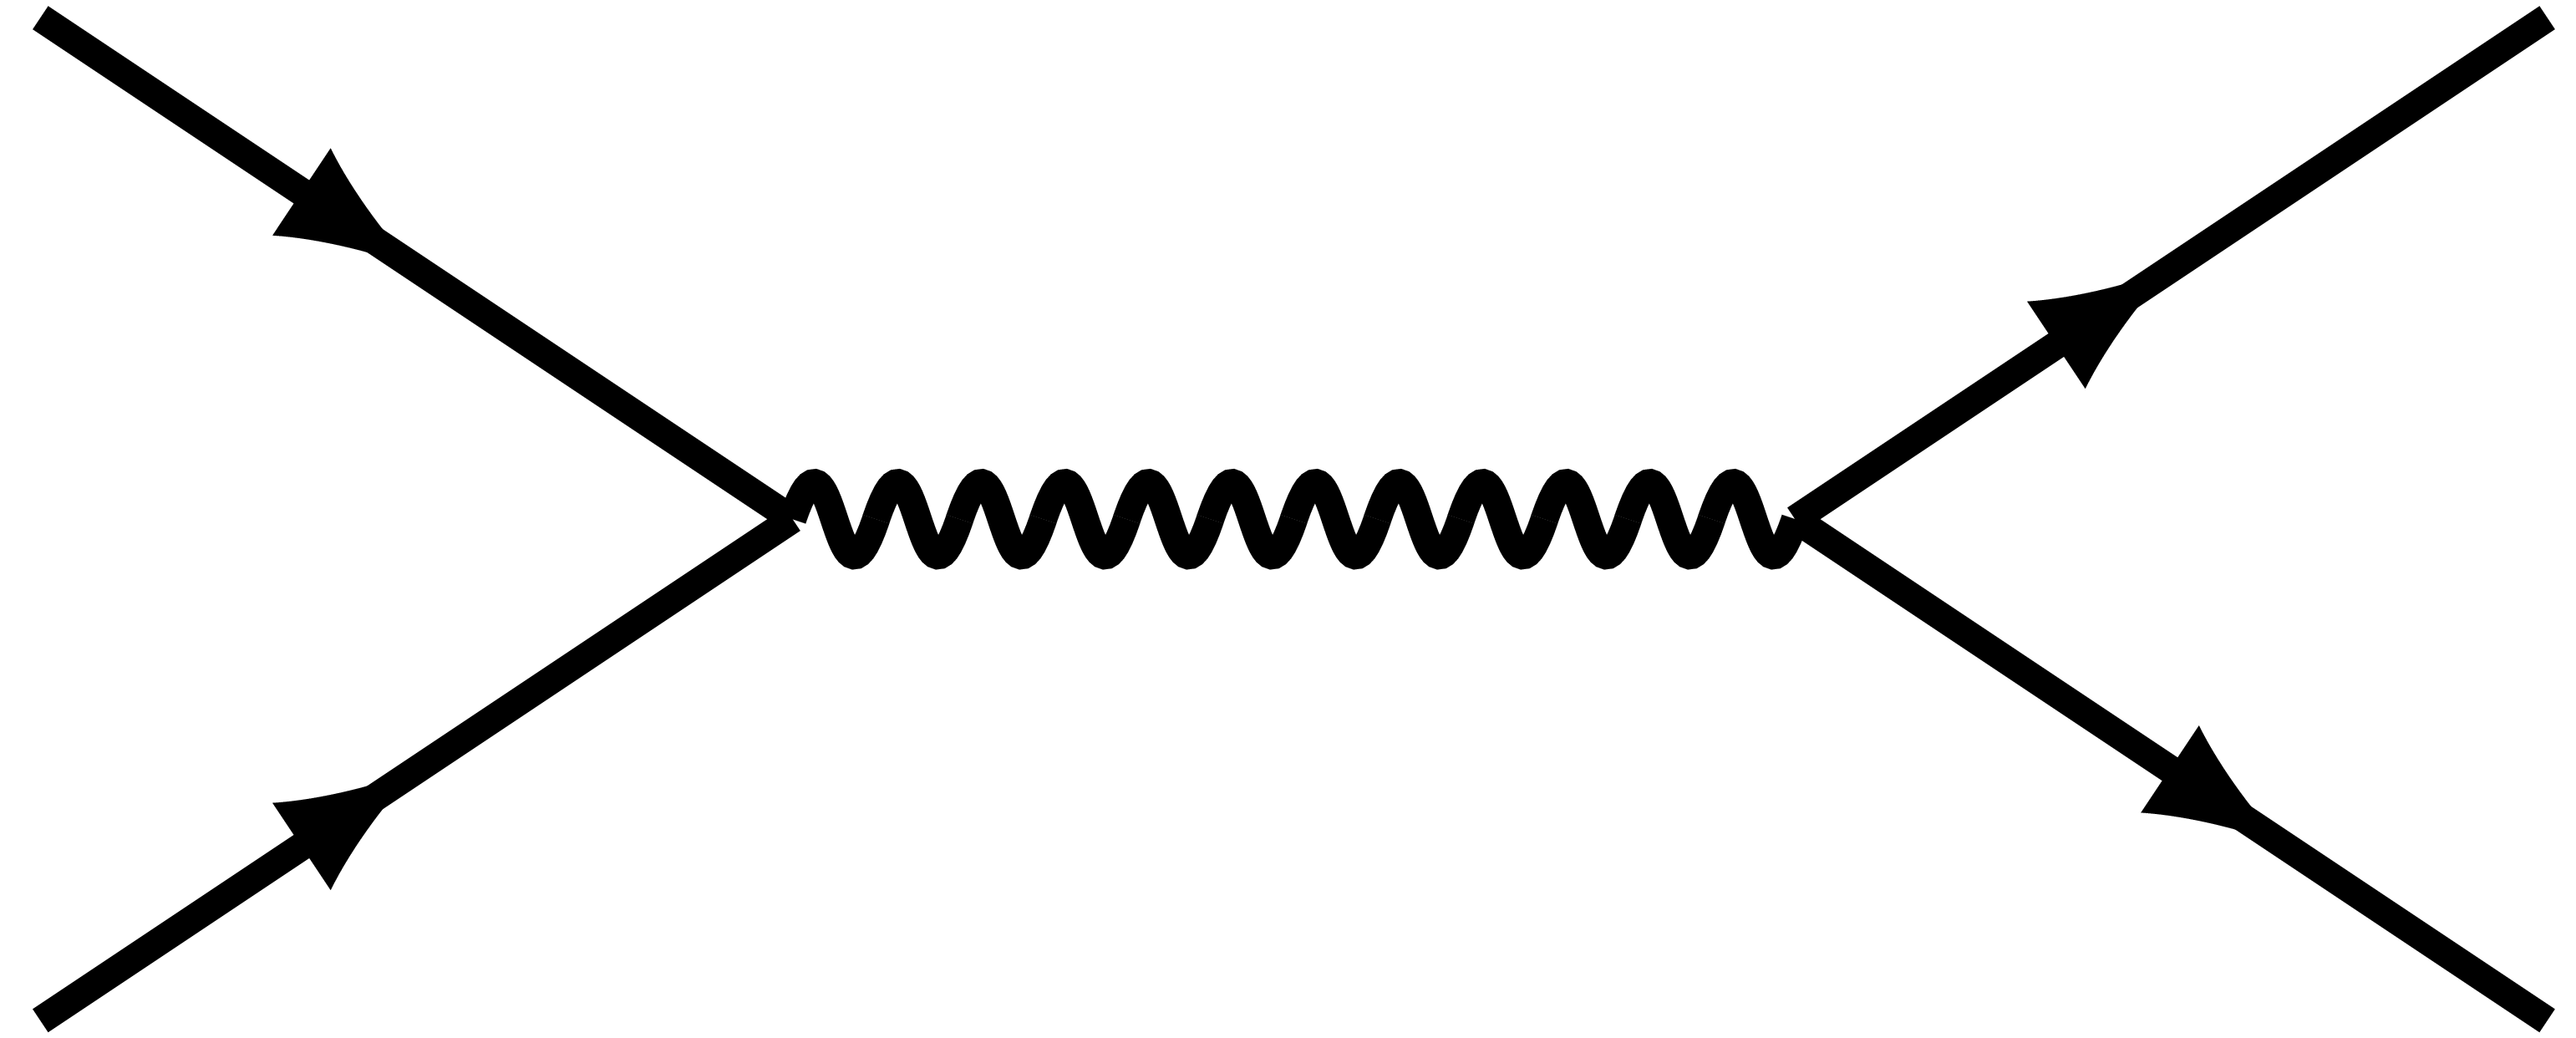
\includegraphics[align=c,width=1.2in]{CC}&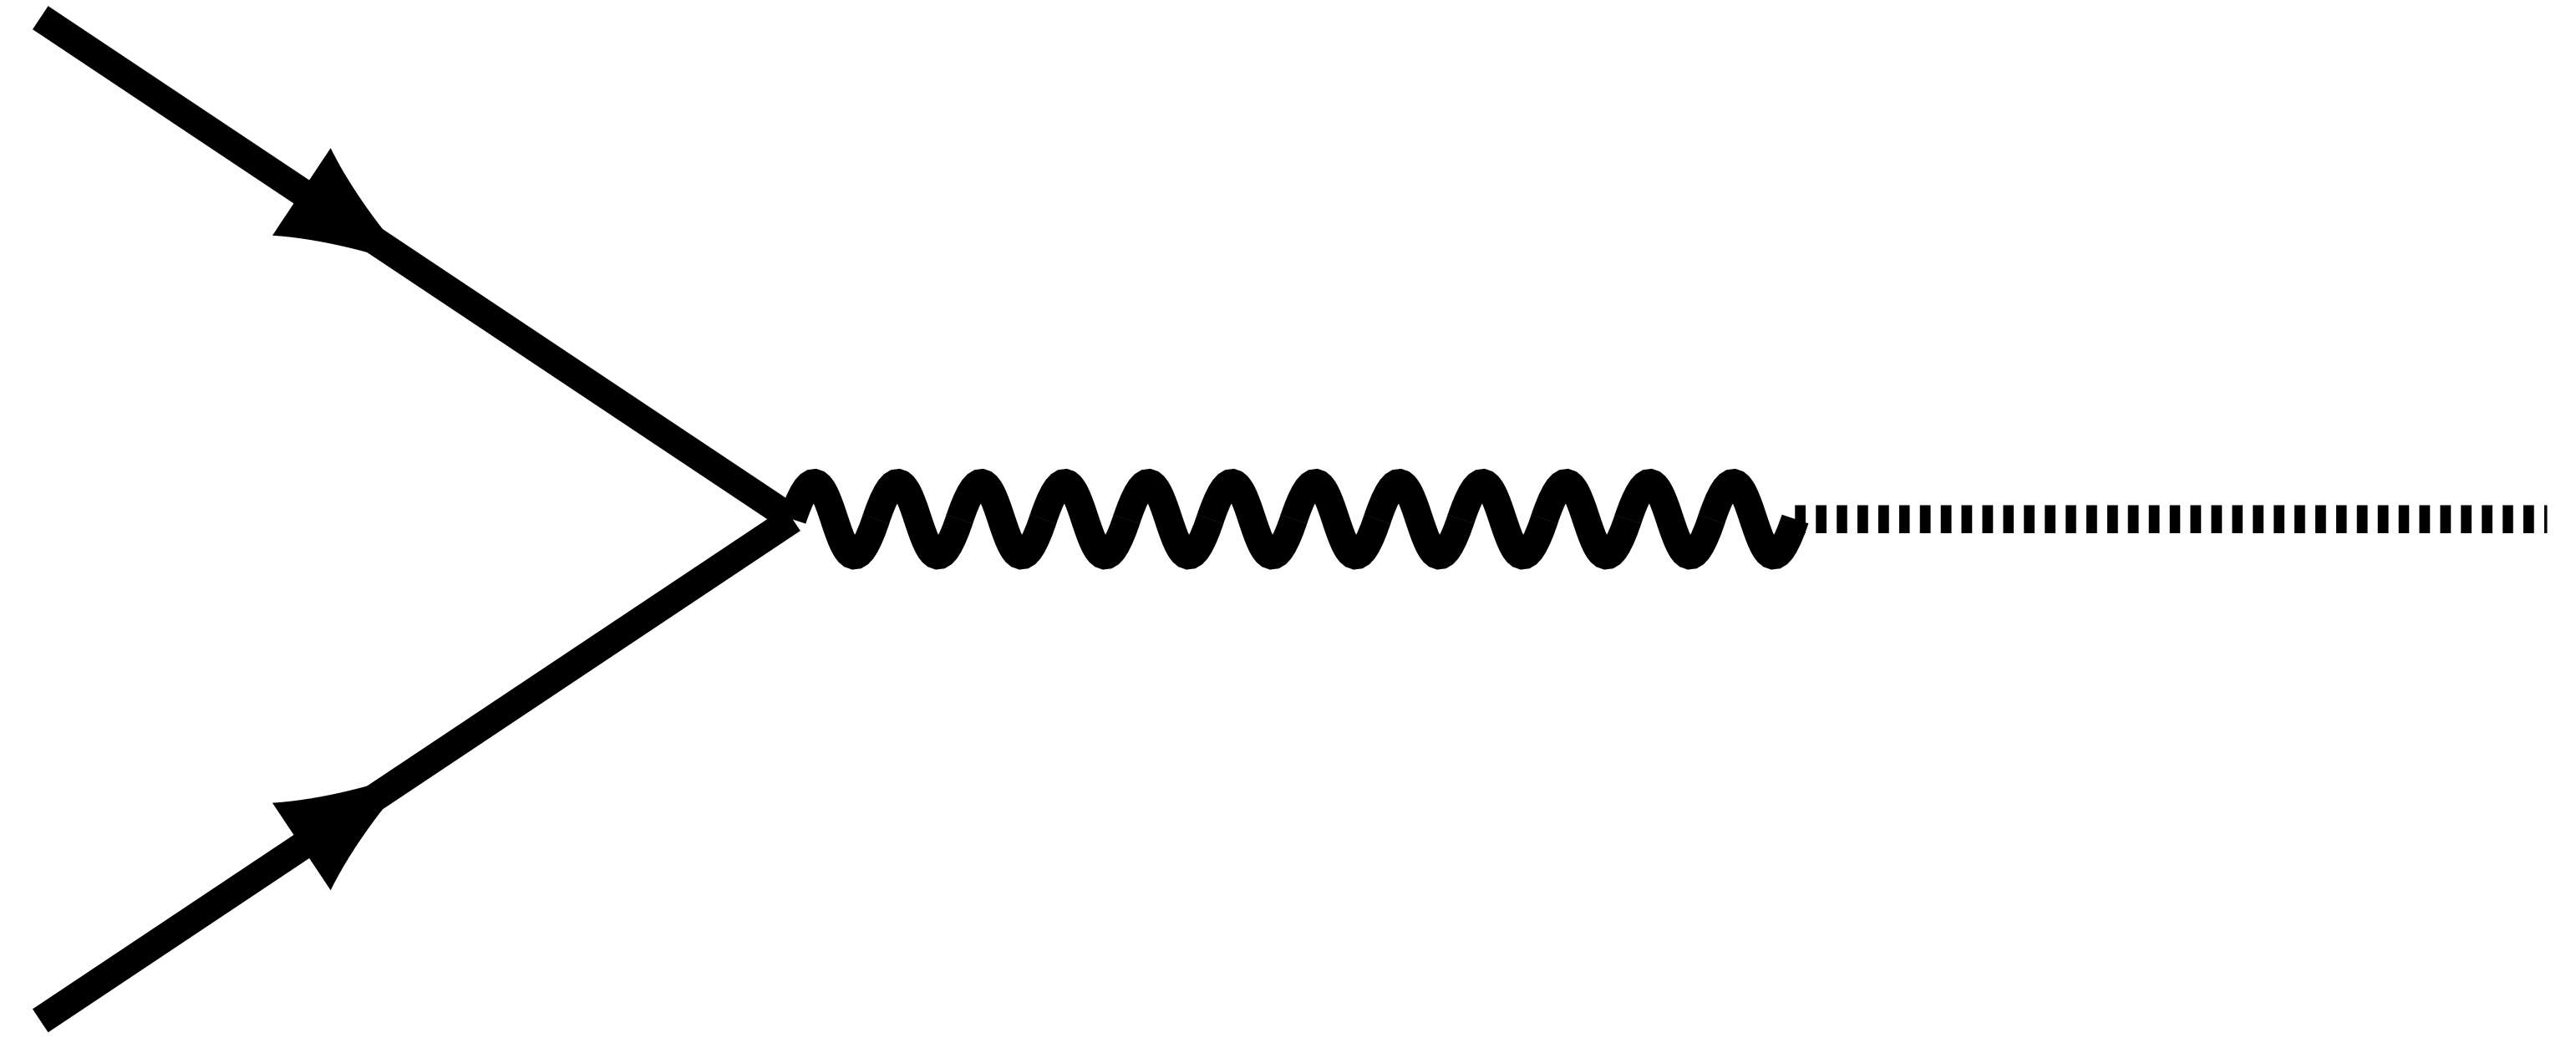
\includegraphics[align=c,width=1.2in]{CD}&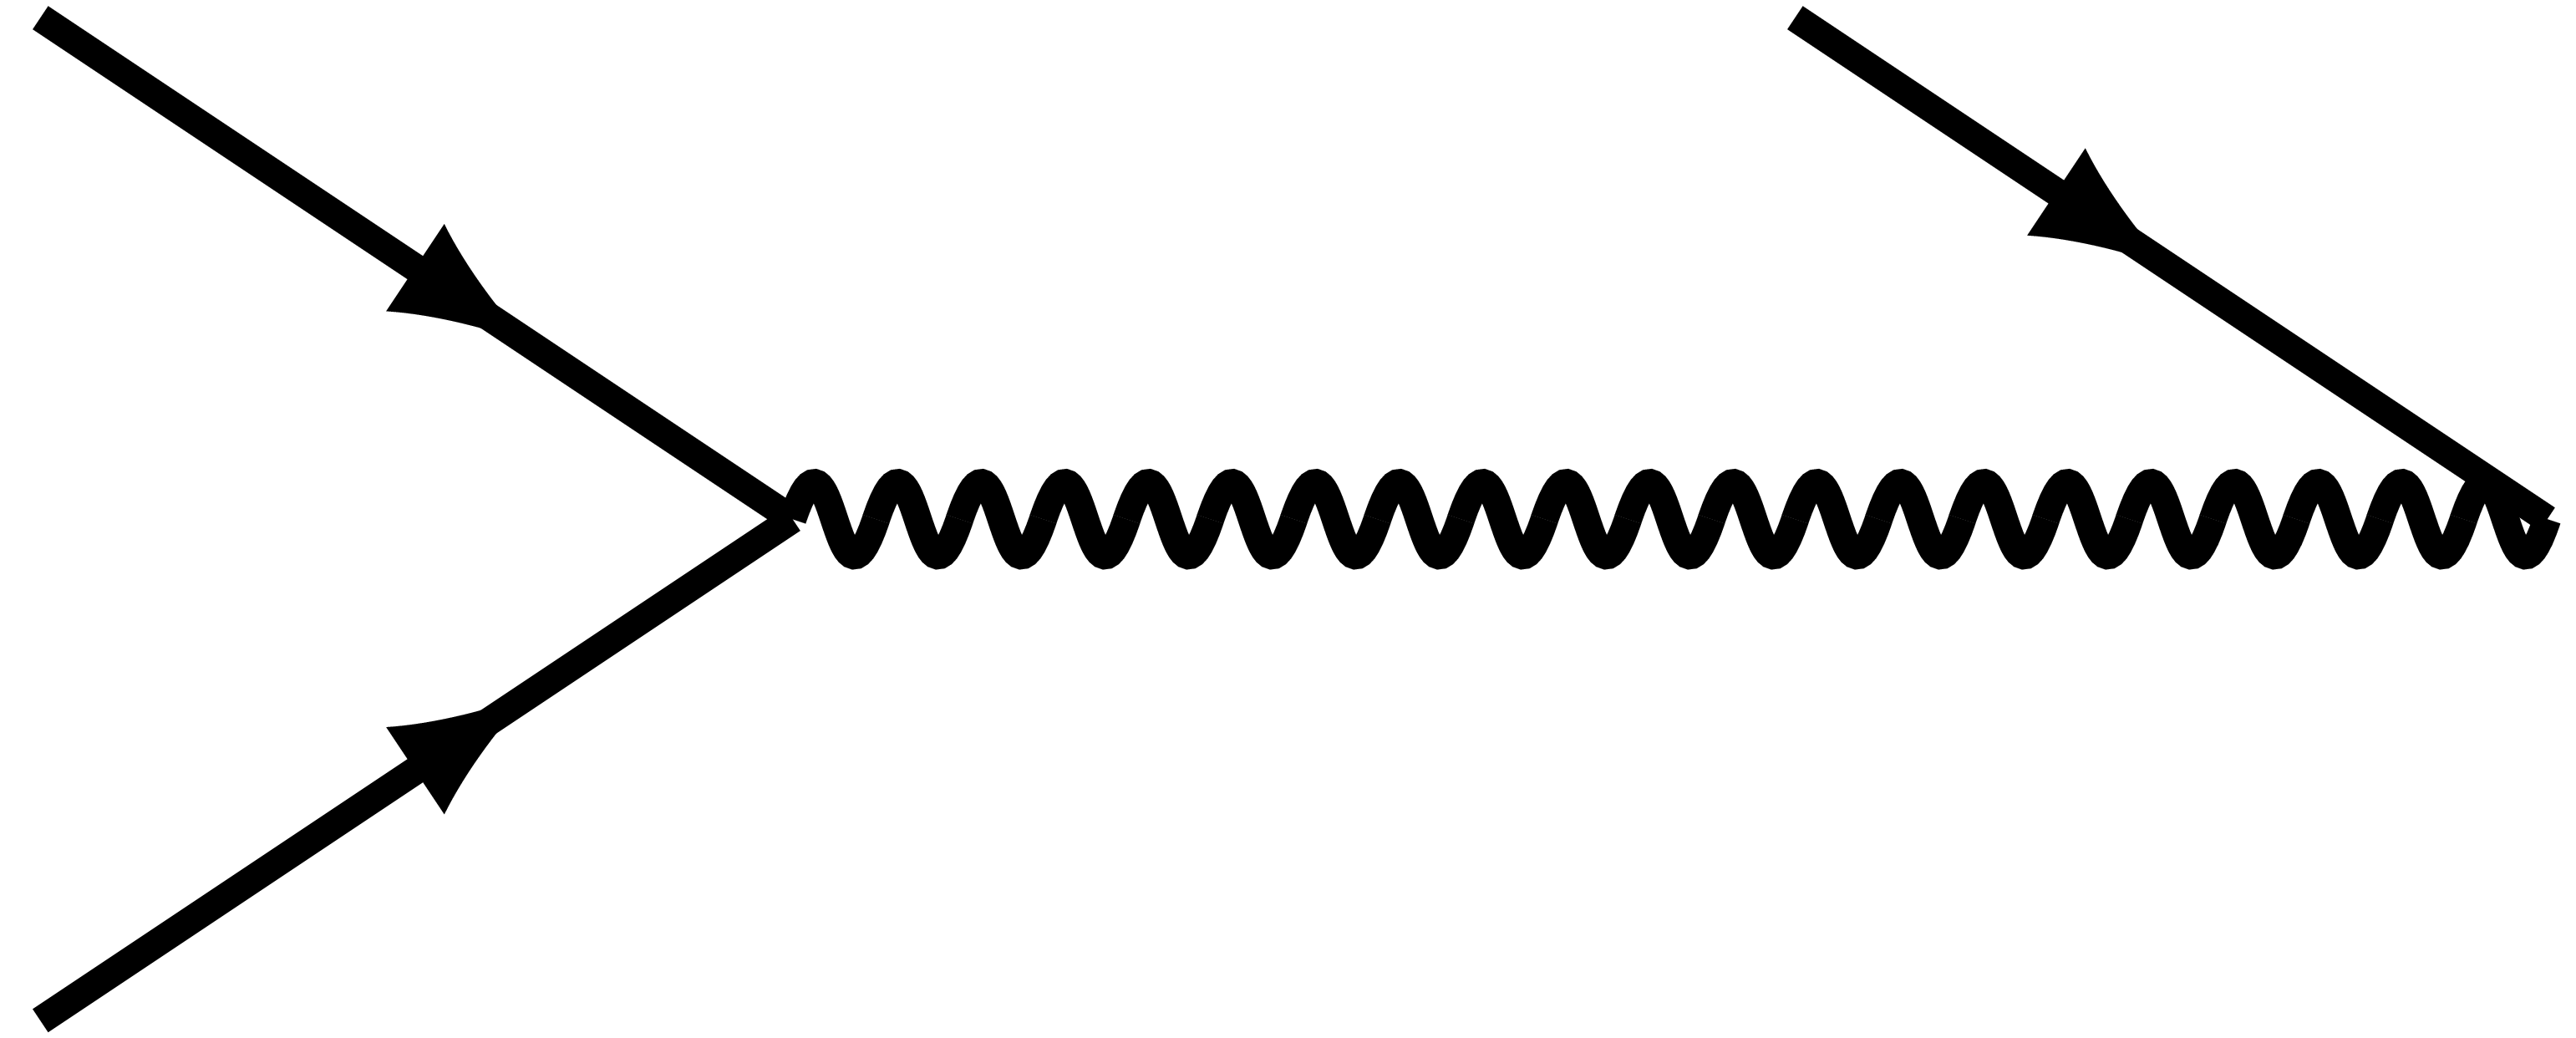
\includegraphics[align=c,width=1.2in]{CE}&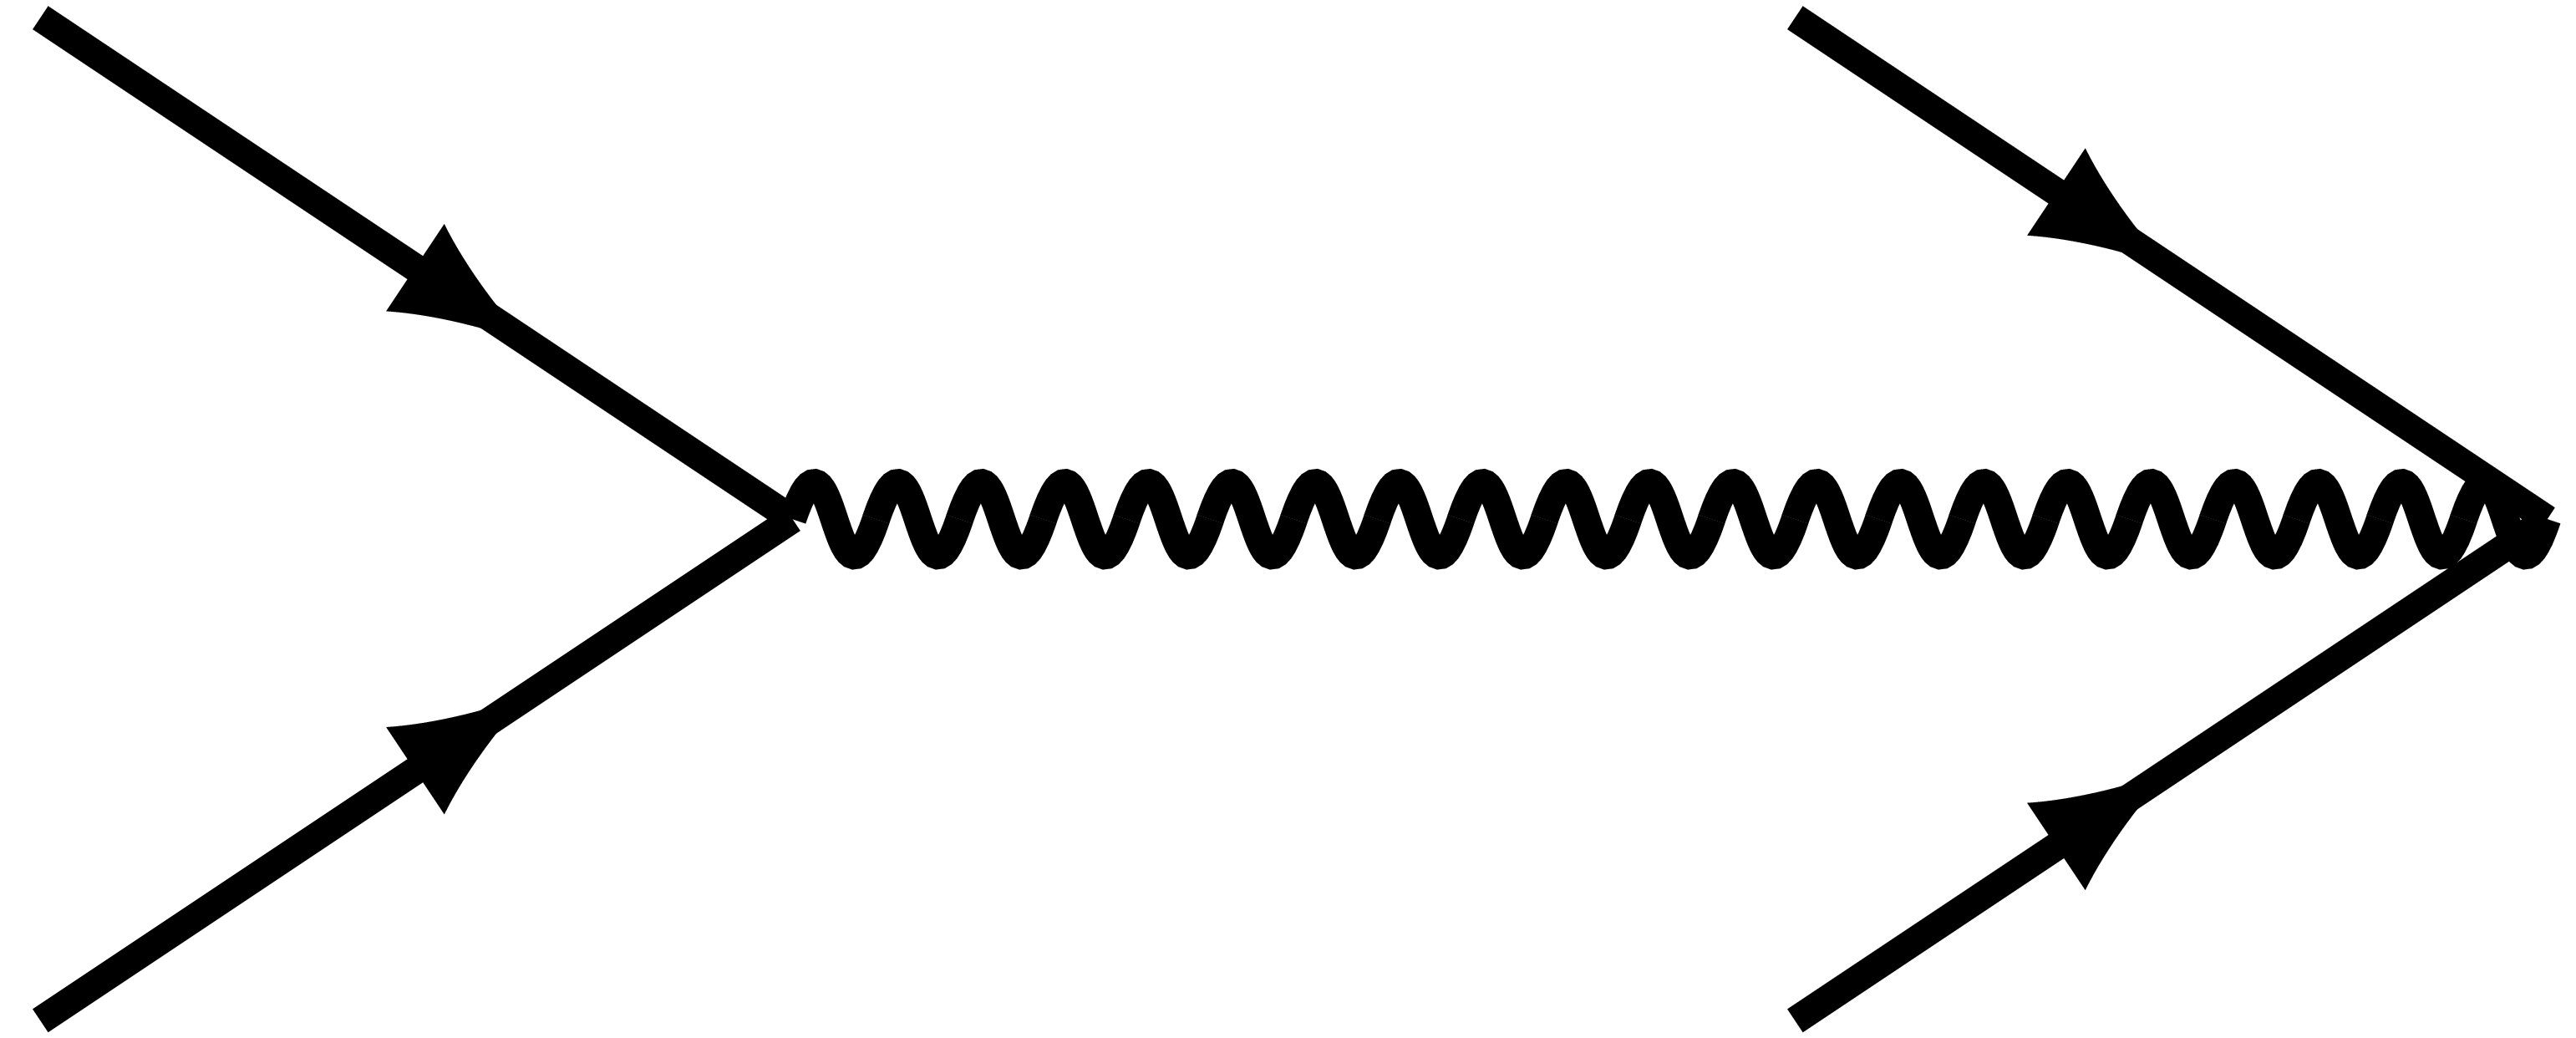
\includegraphics[align=c,width=1.2in]{CF}\\
        $D$ & 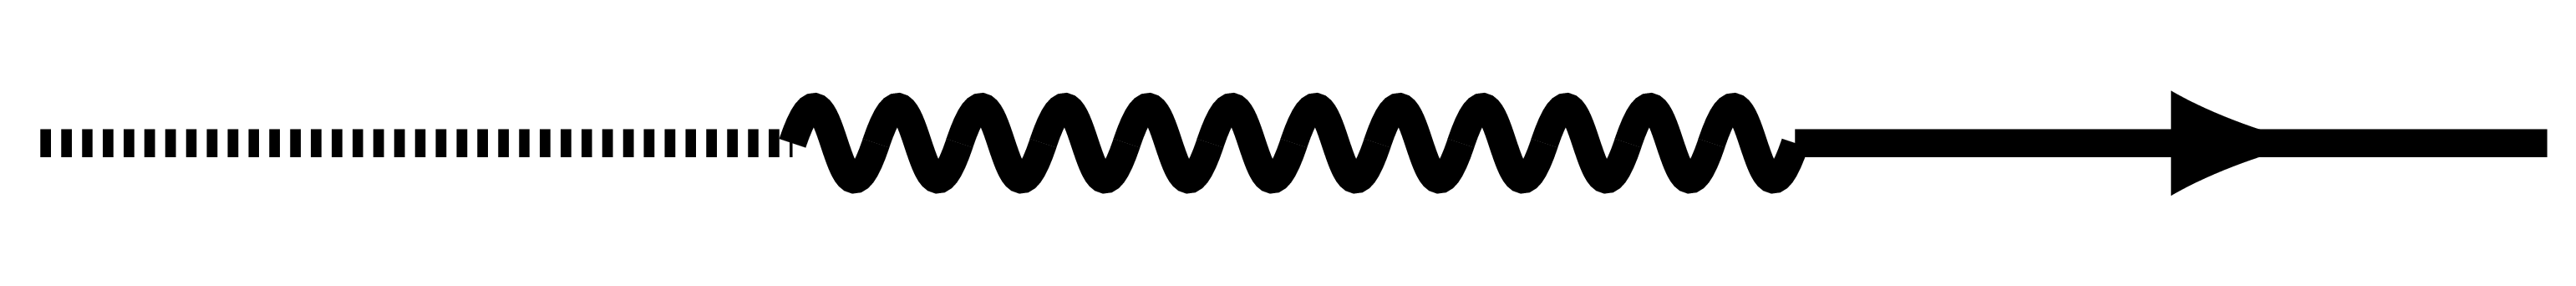
\includegraphics[align=c,width=1.2in]{DA}&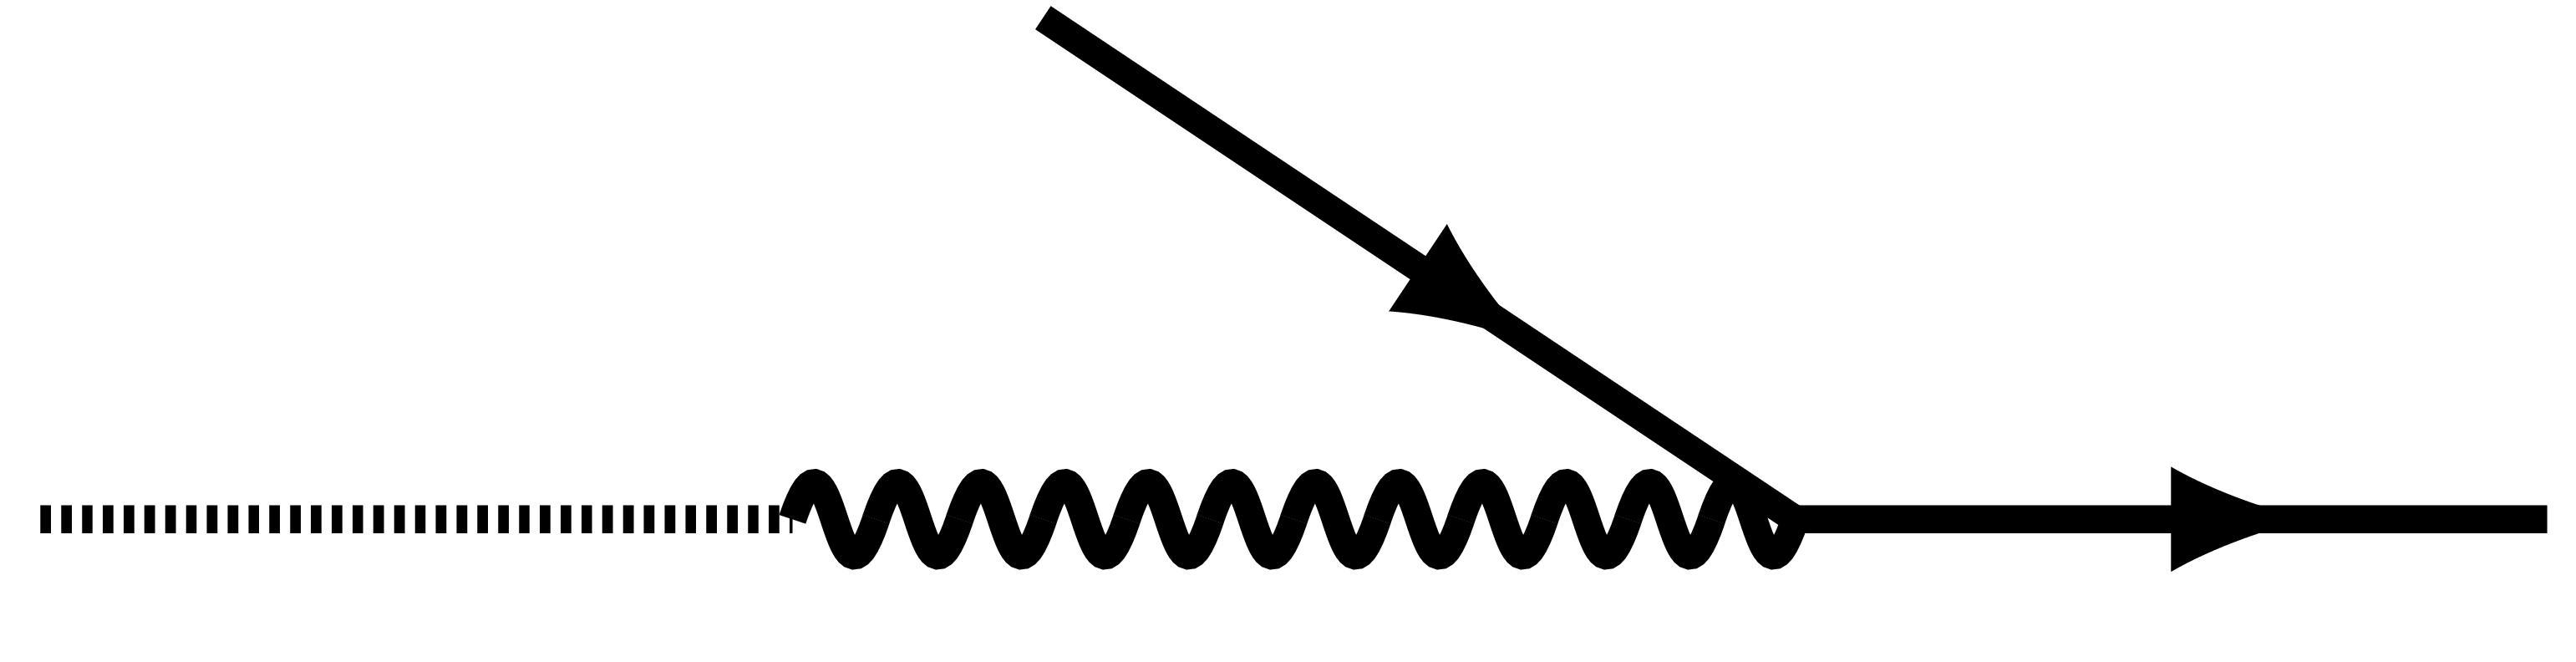
\includegraphics[align=c,width=1.2in]{DB}&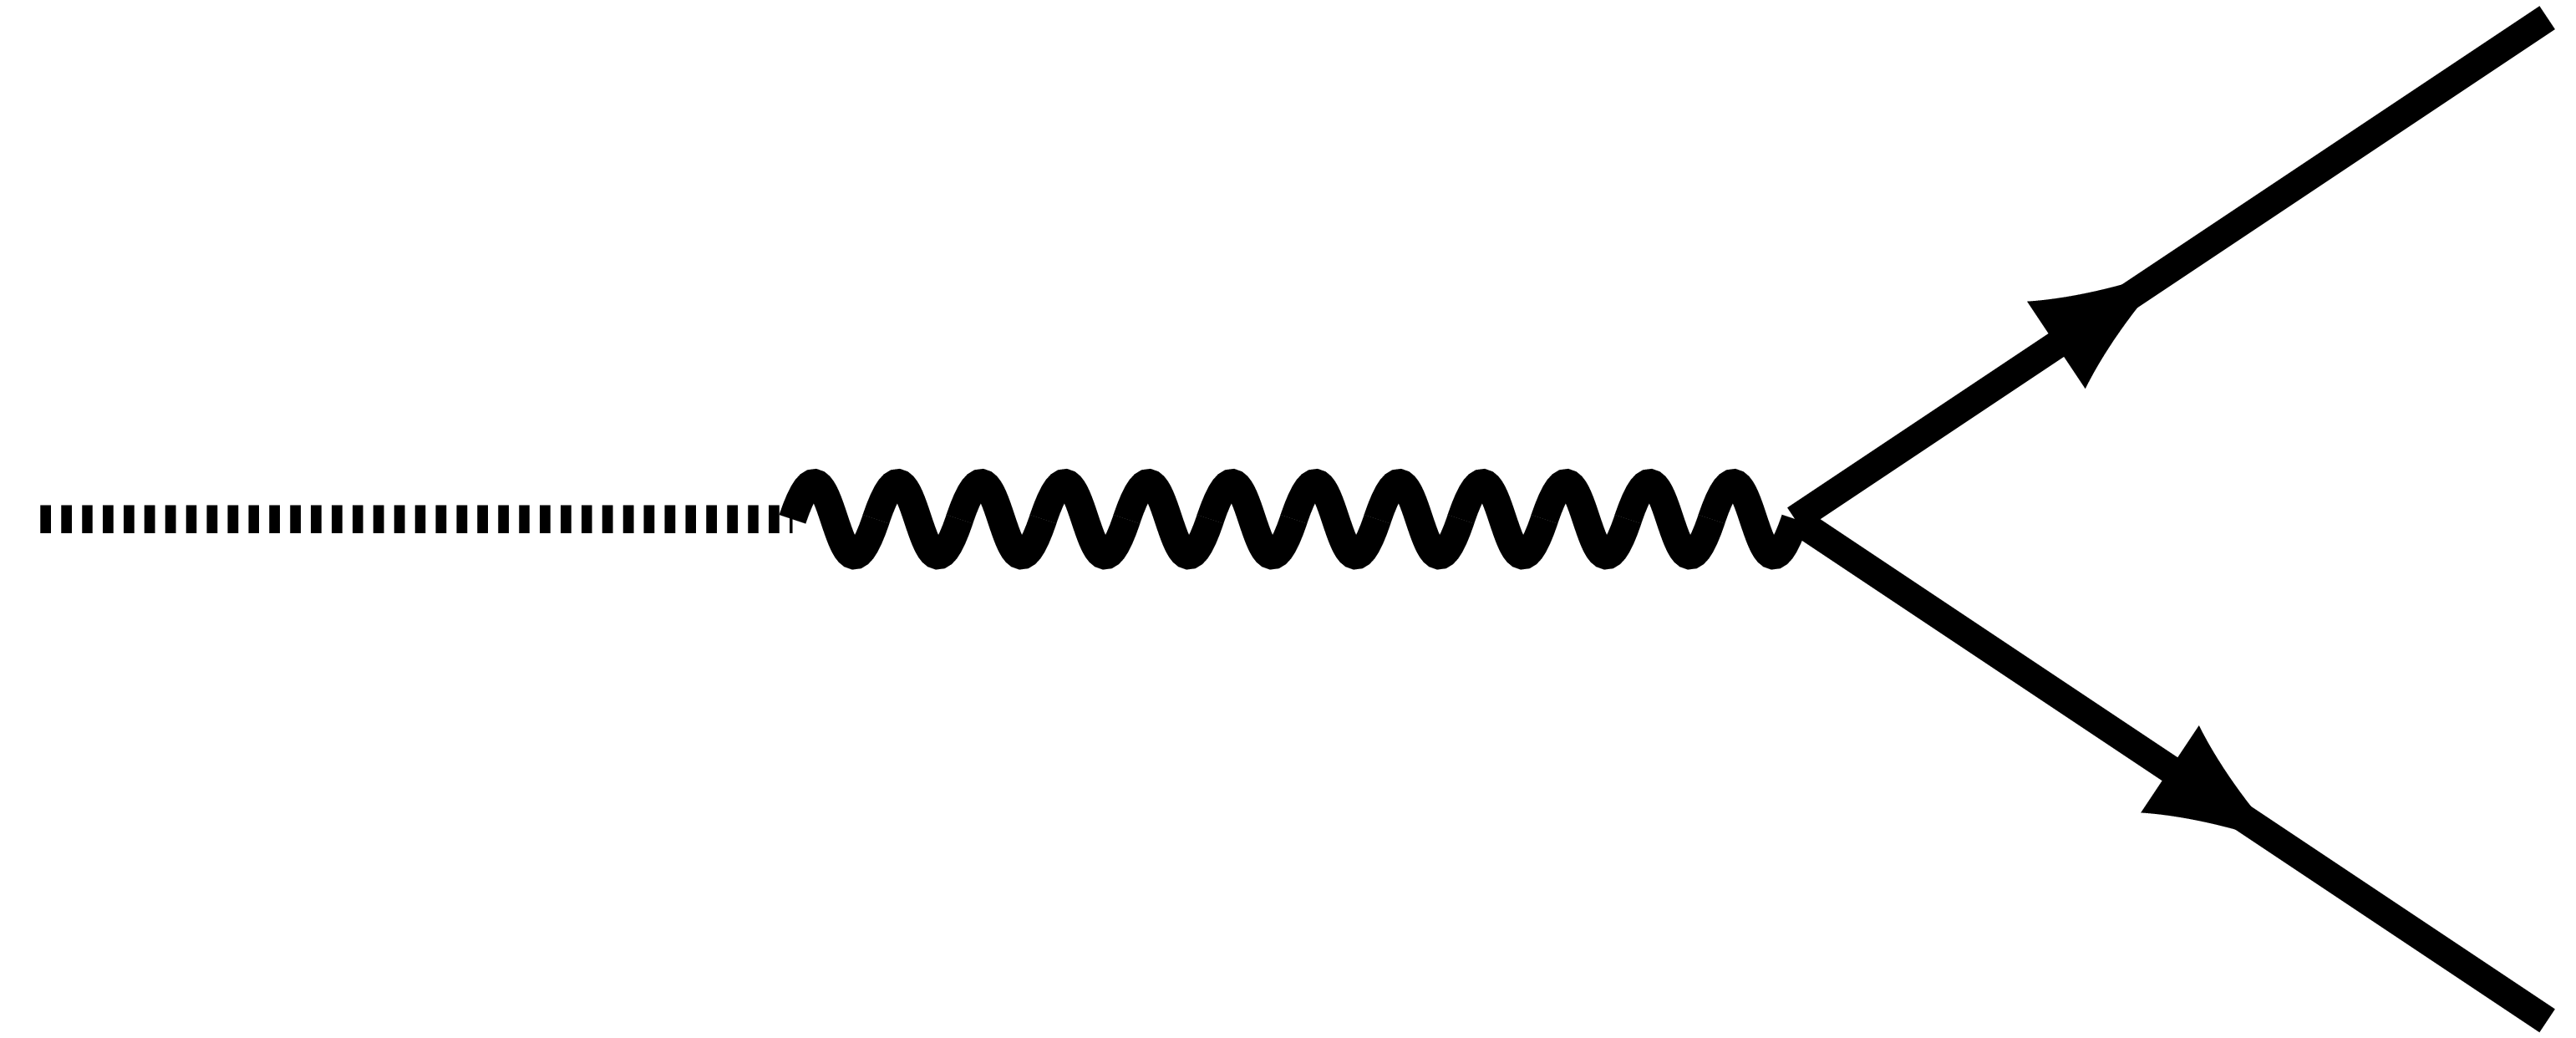
\includegraphics[align=c,width=1.2in]{DC}&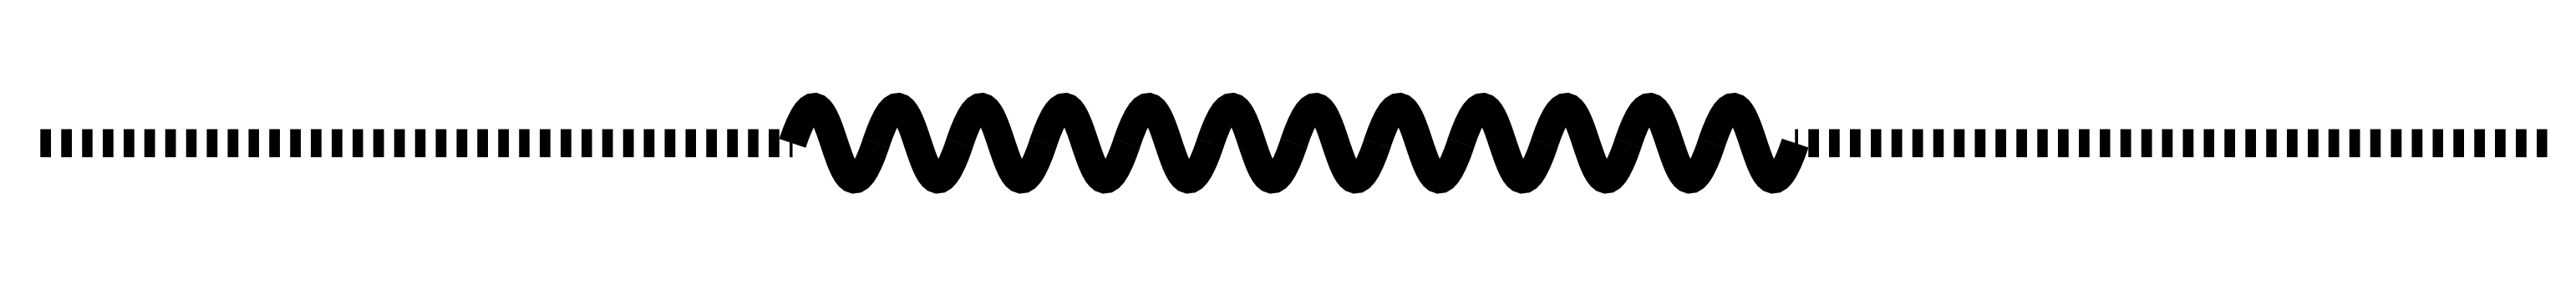
\includegraphics[align=c,width=1.2in]{DD}&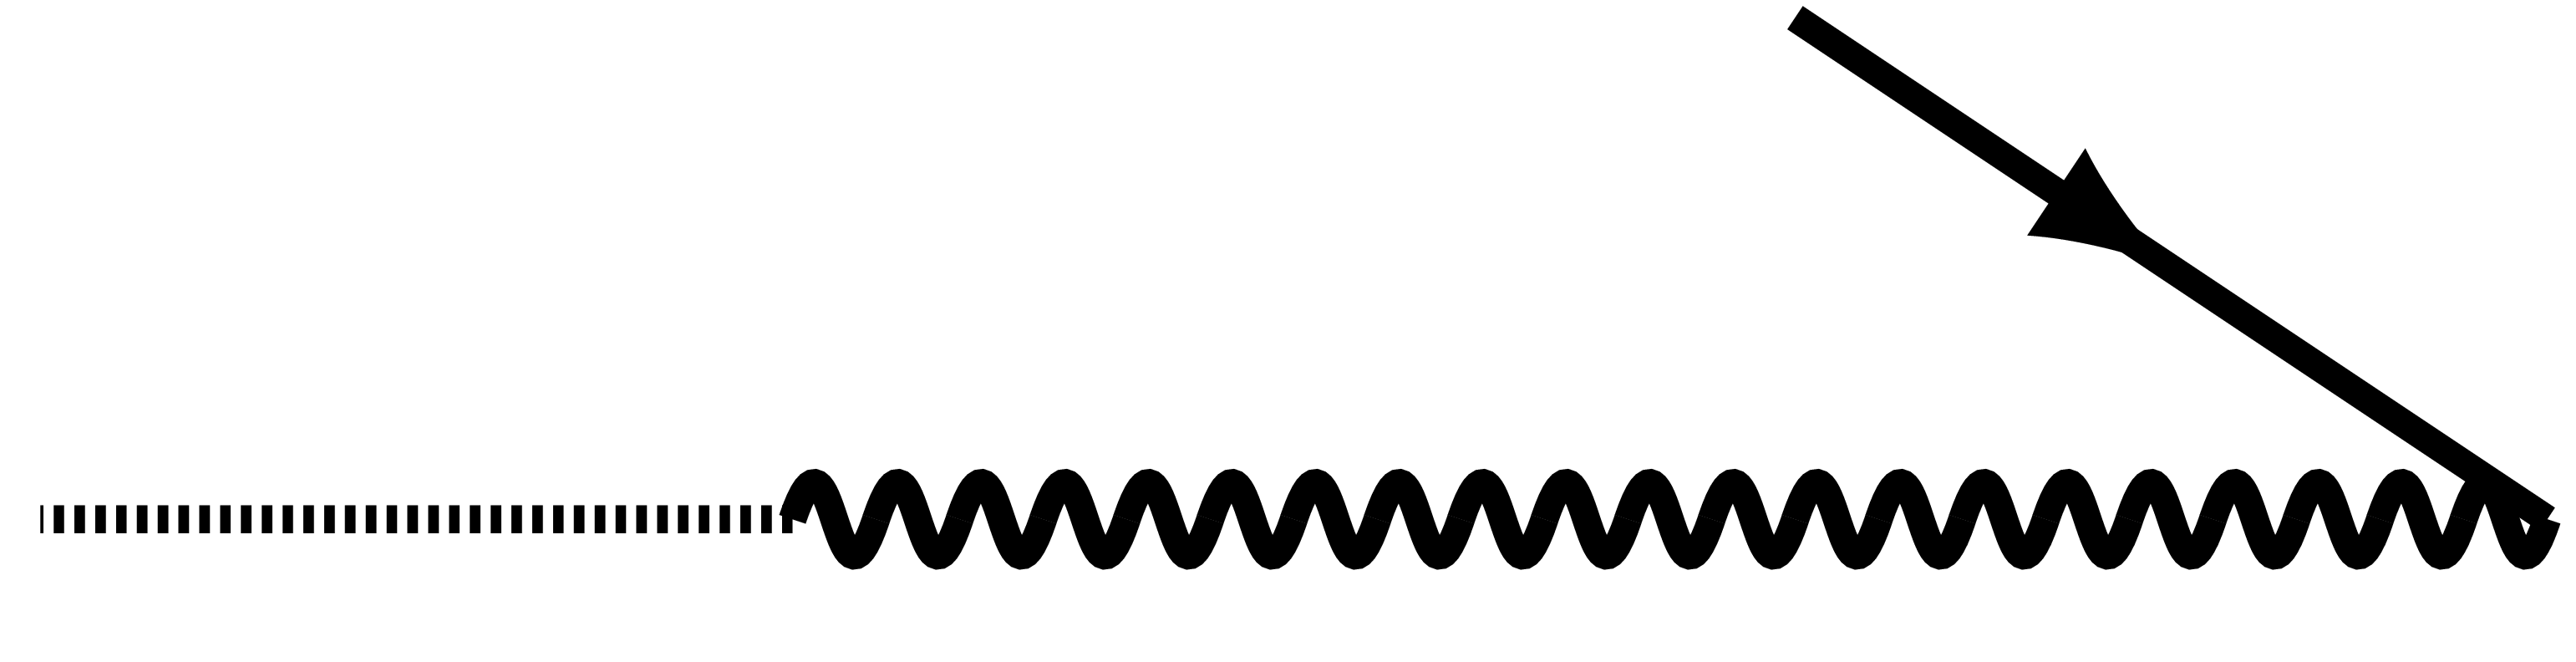
\includegraphics[align=c,width=1.2in]{DE}&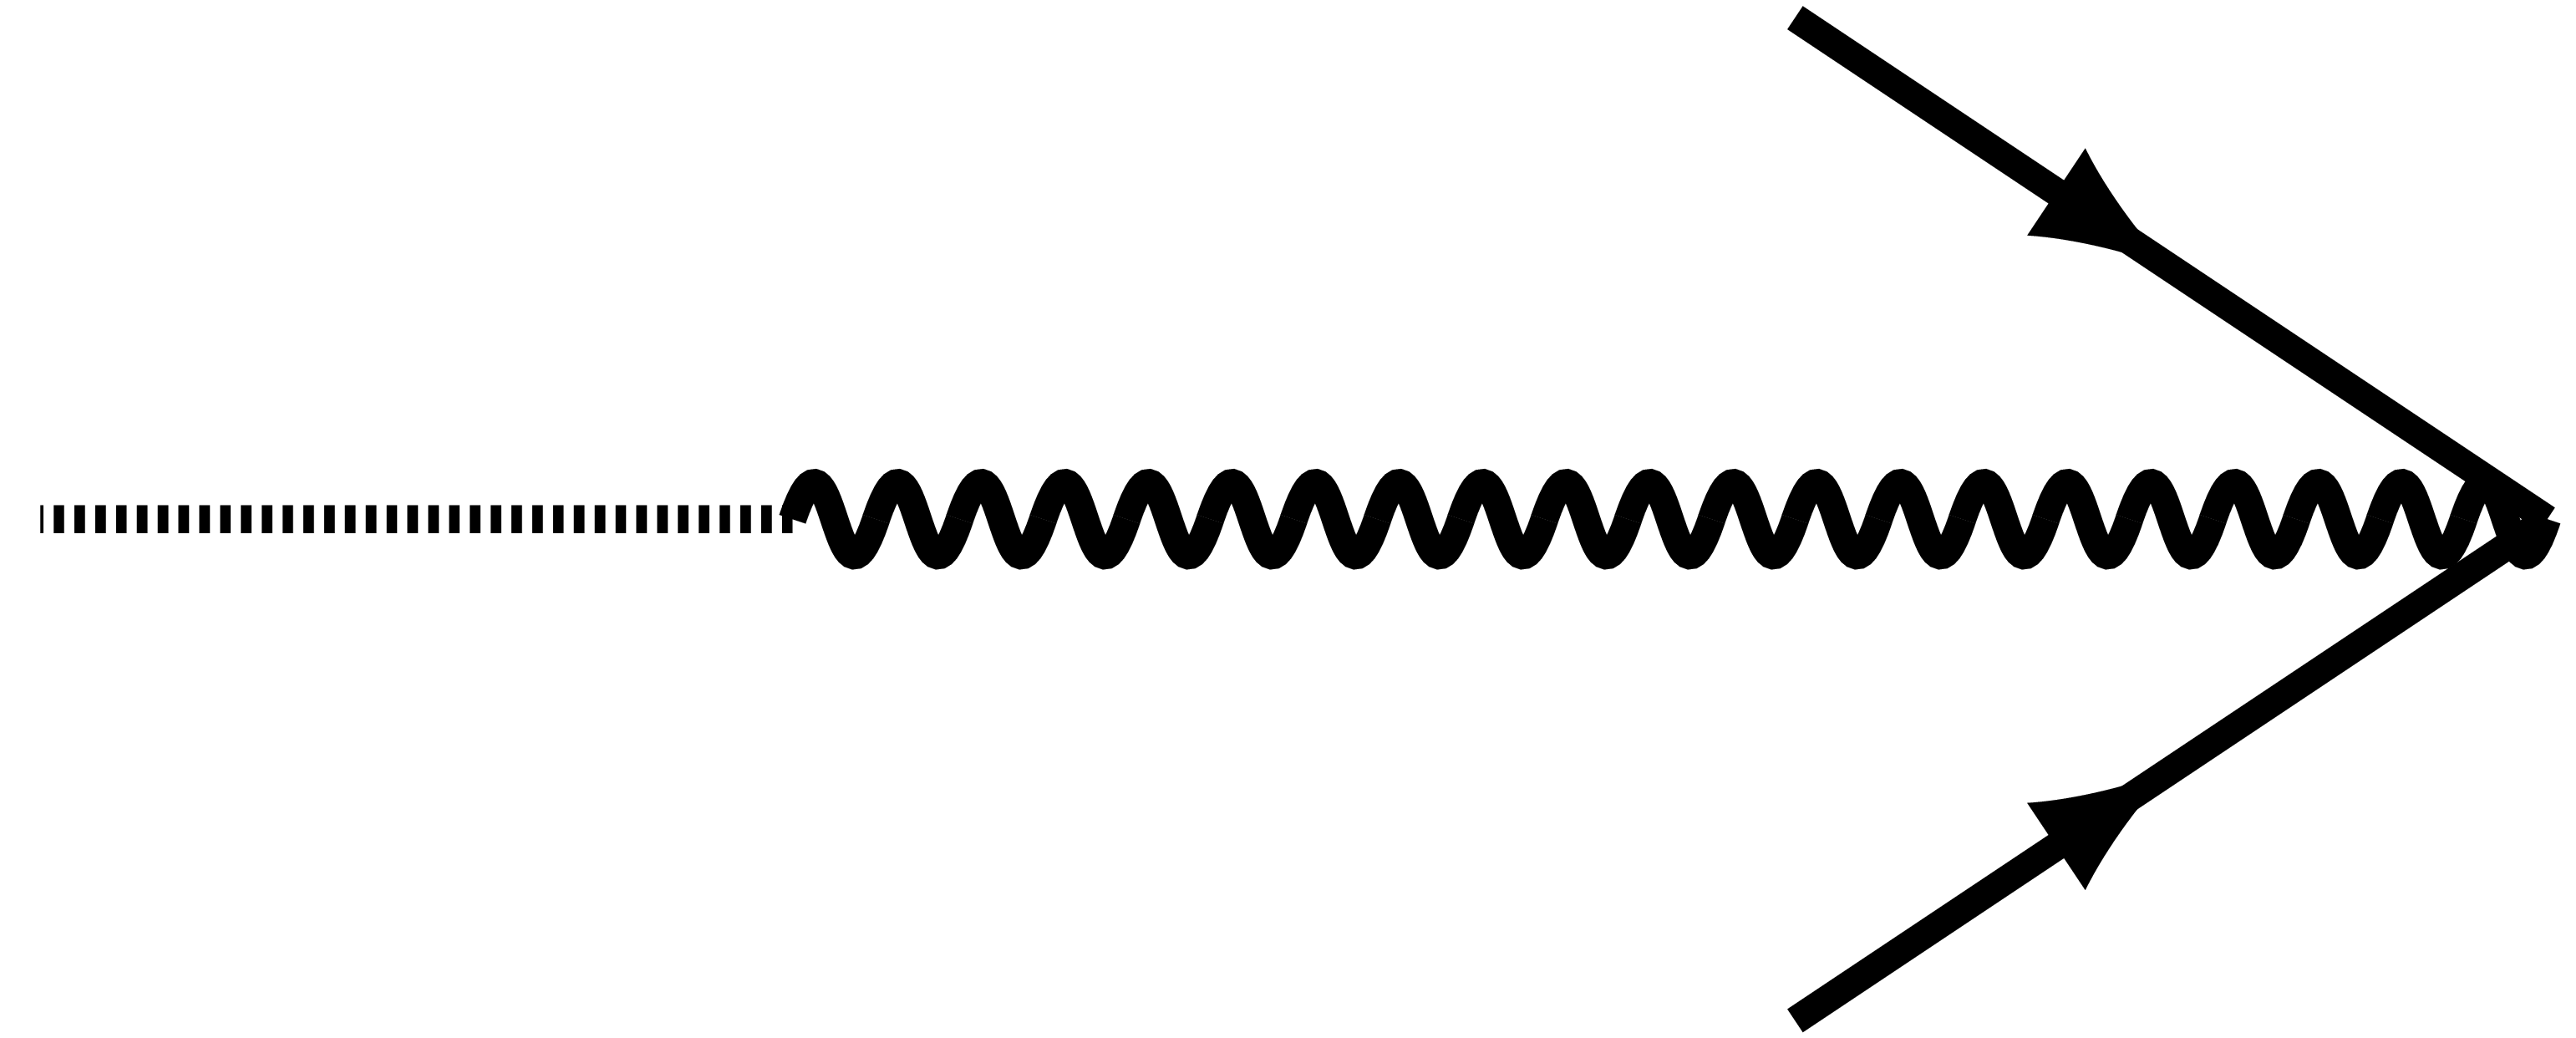
\includegraphics[align=c,width=1.2in]{DF}\\
        $E$ & 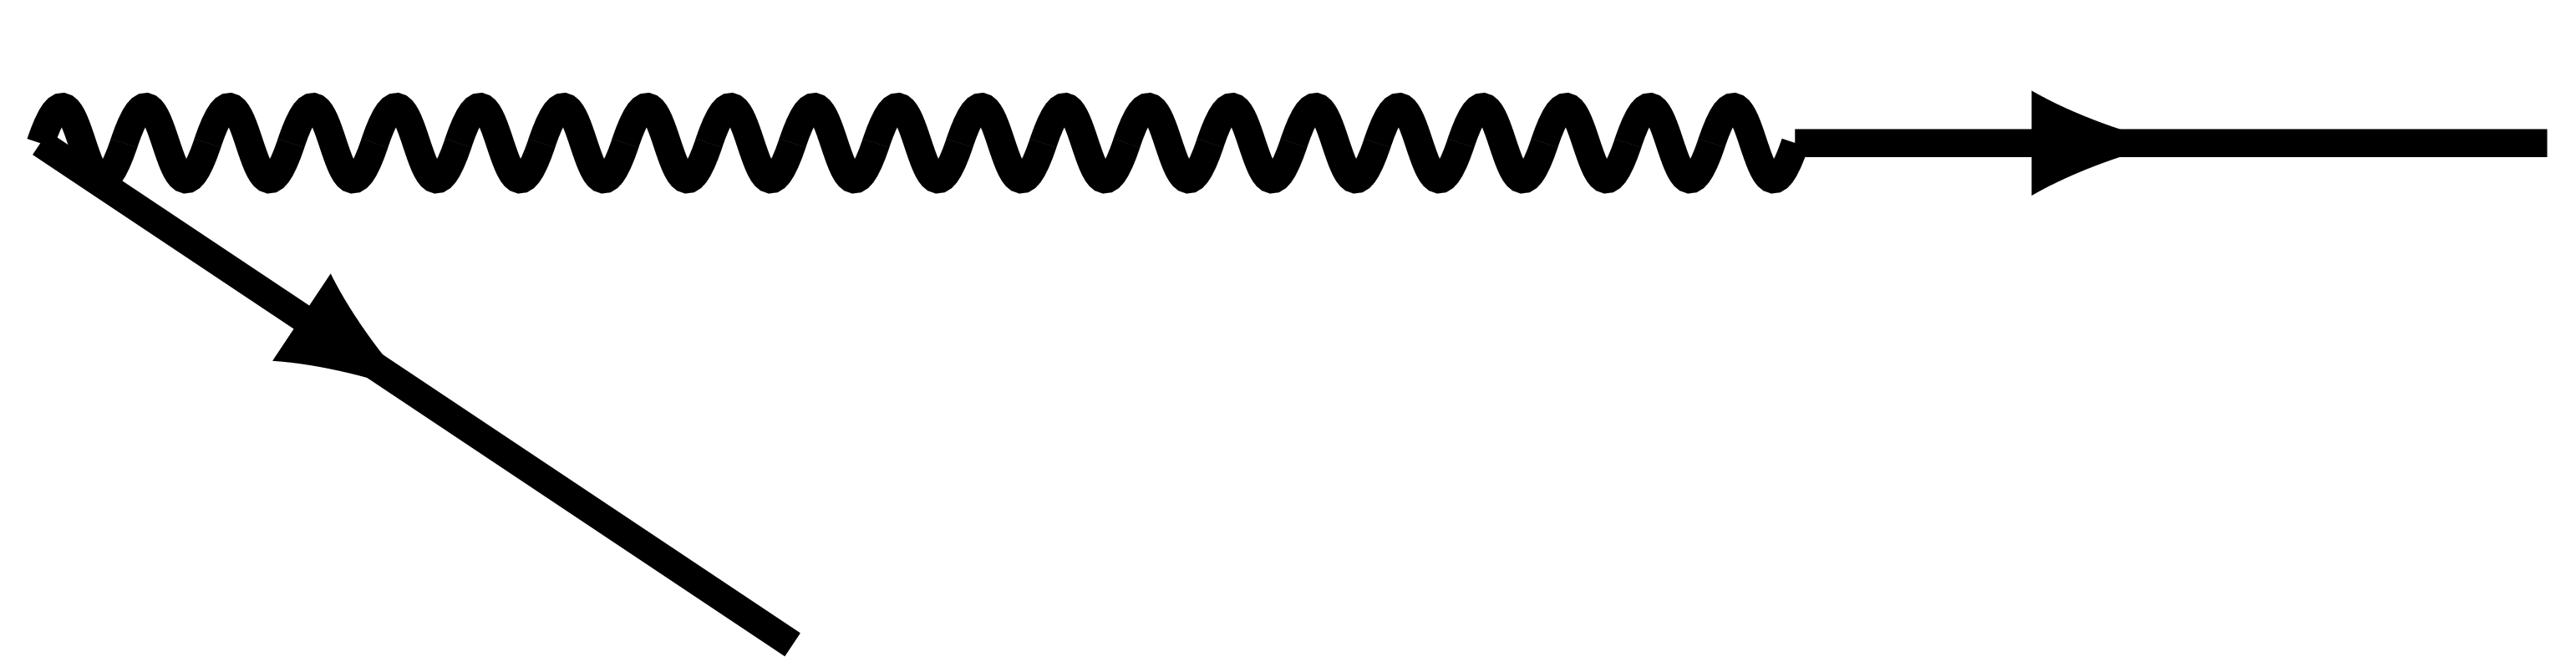
\includegraphics[align=c,width=1.2in]{EA}&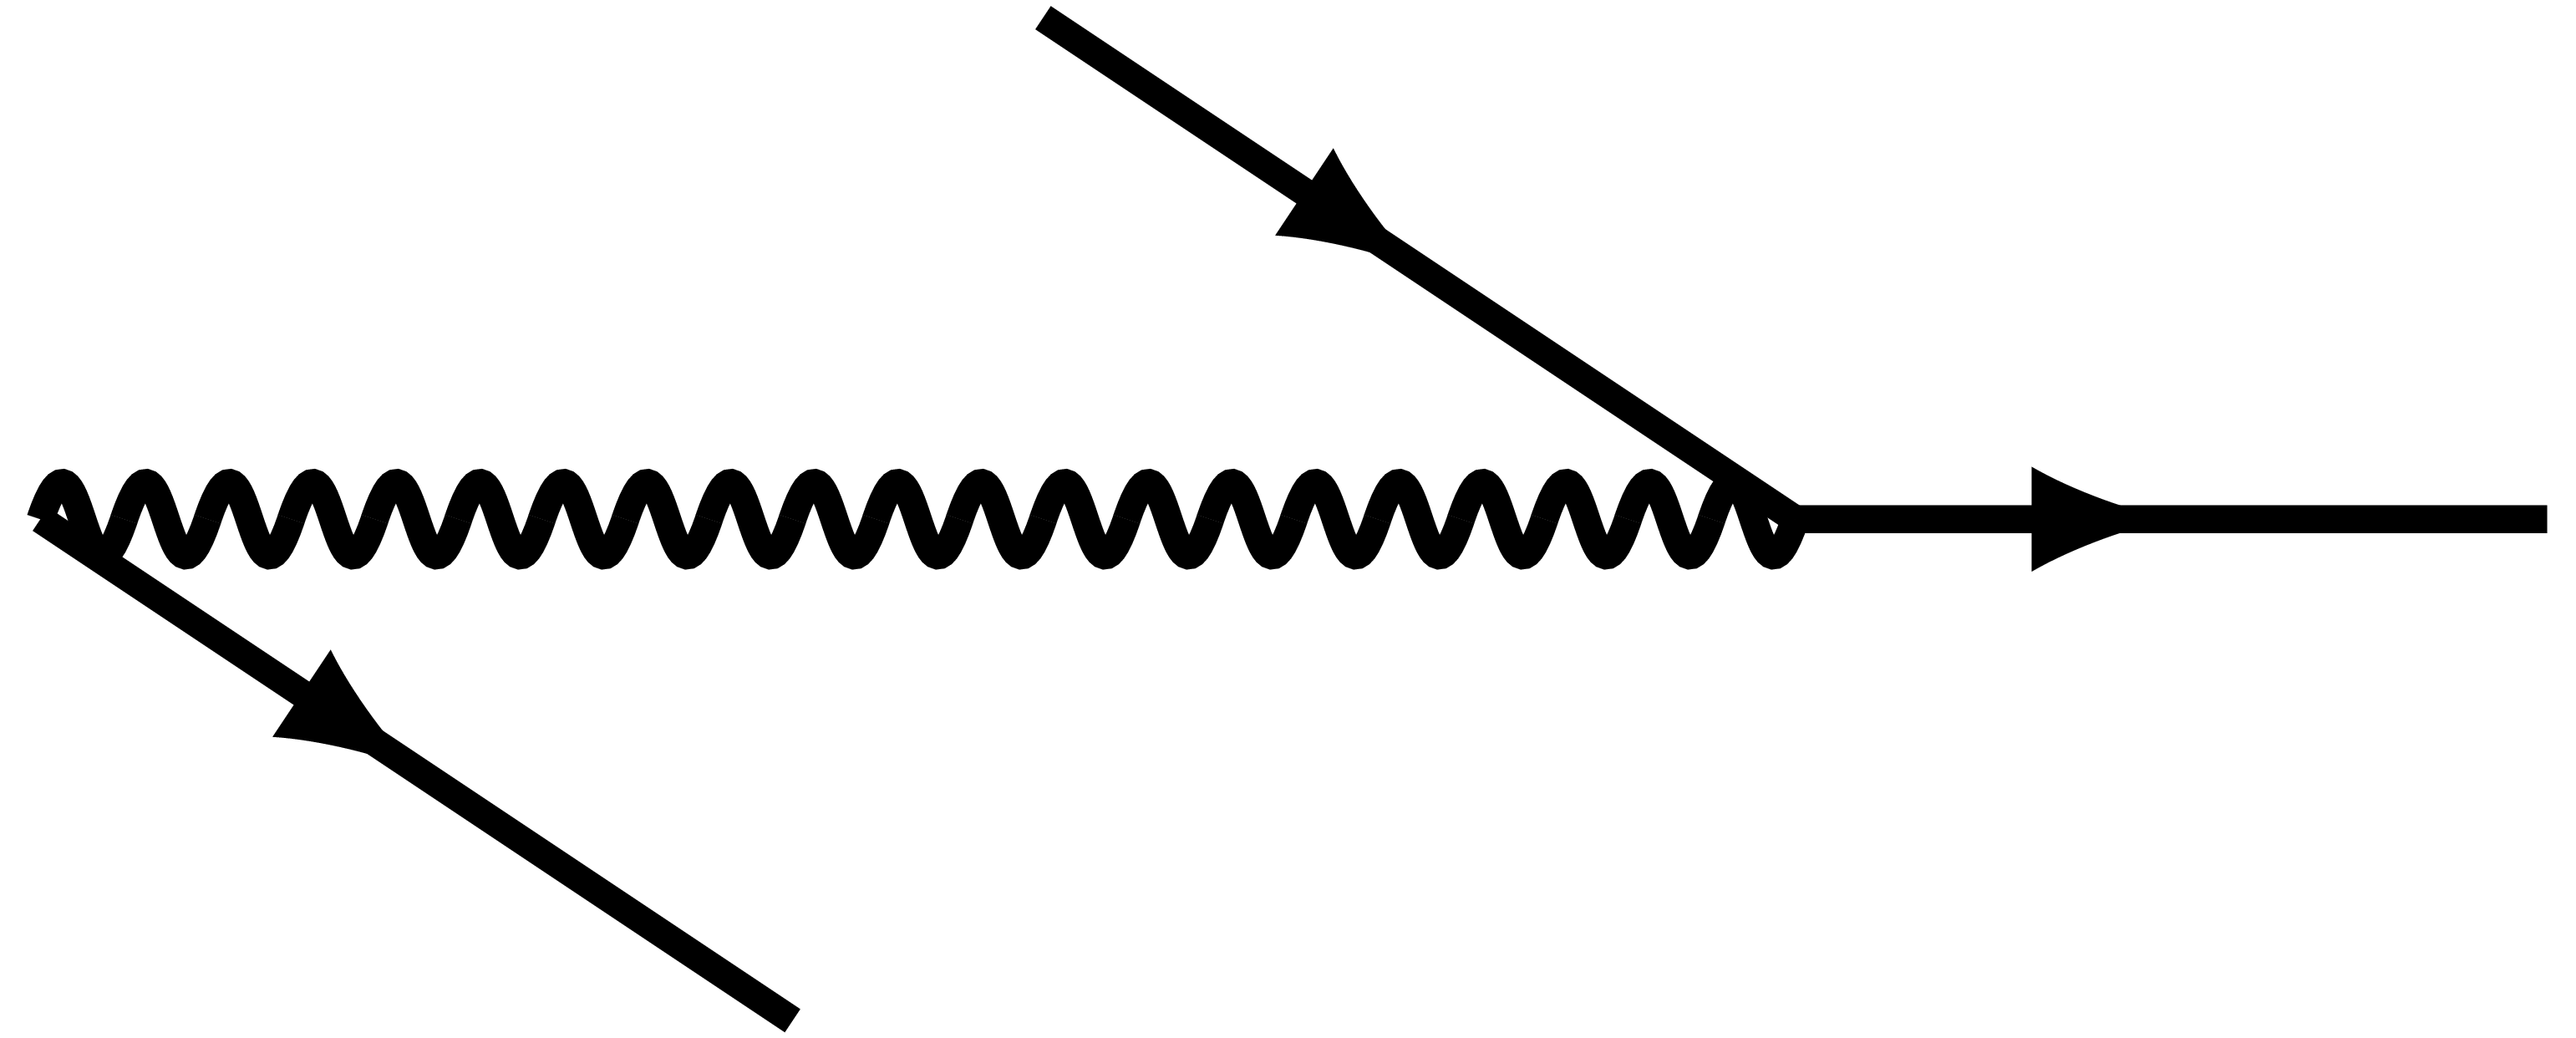
\includegraphics[align=c,width=1.2in]{EB}&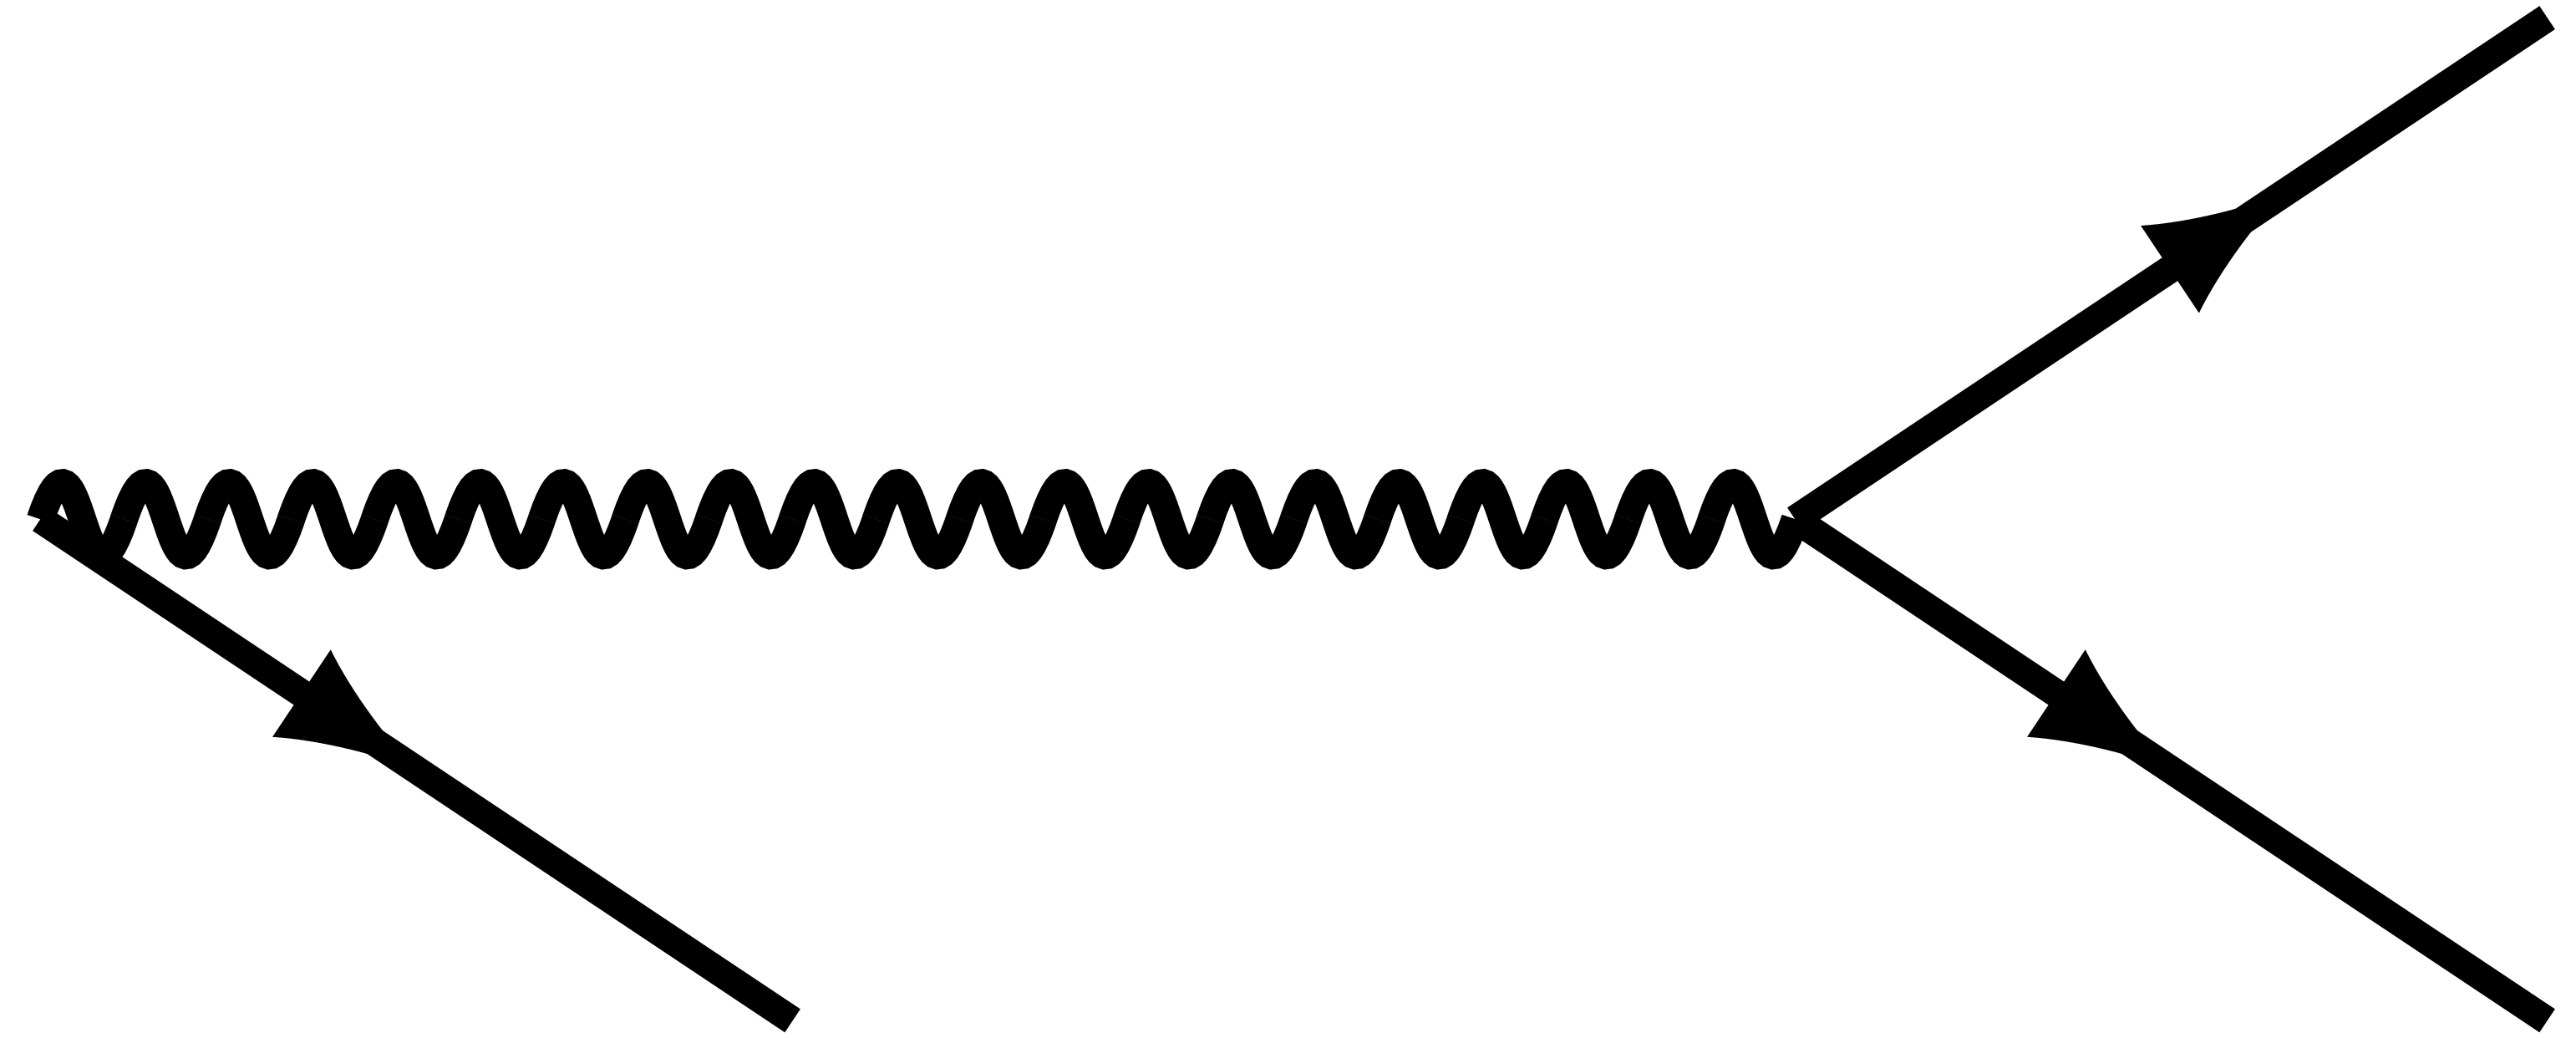
\includegraphics[align=c,width=1.2in]{EC}&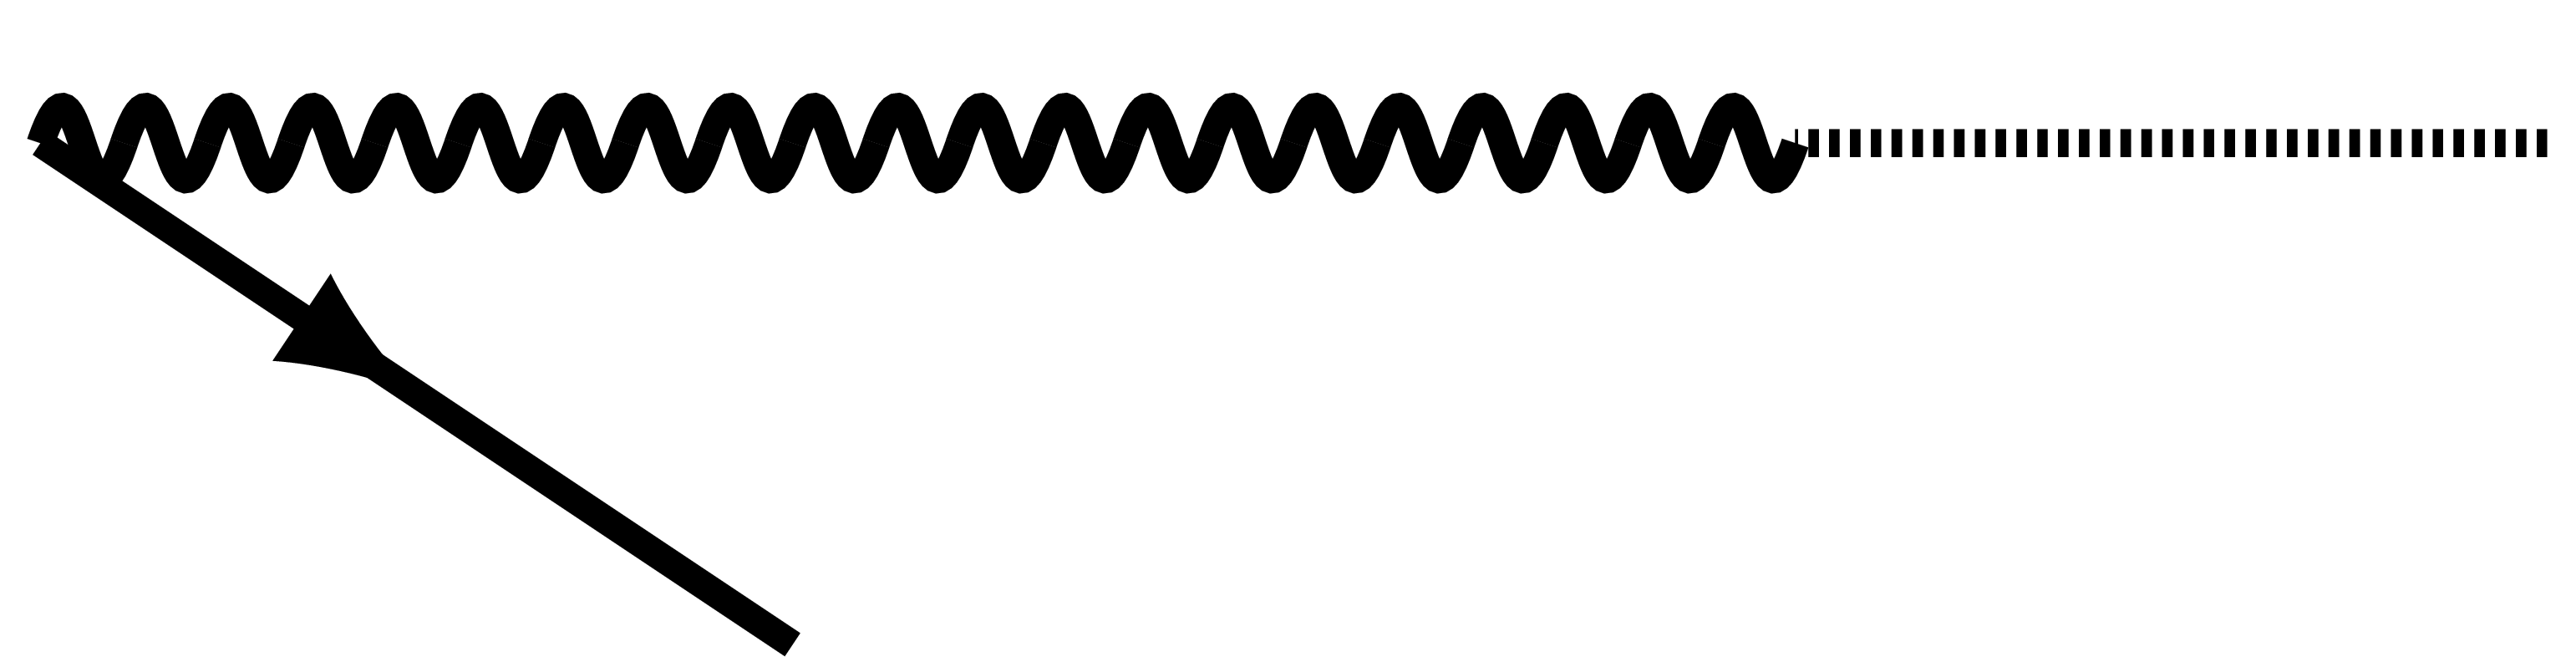
\includegraphics[align=c,width=1.2in]{ED}&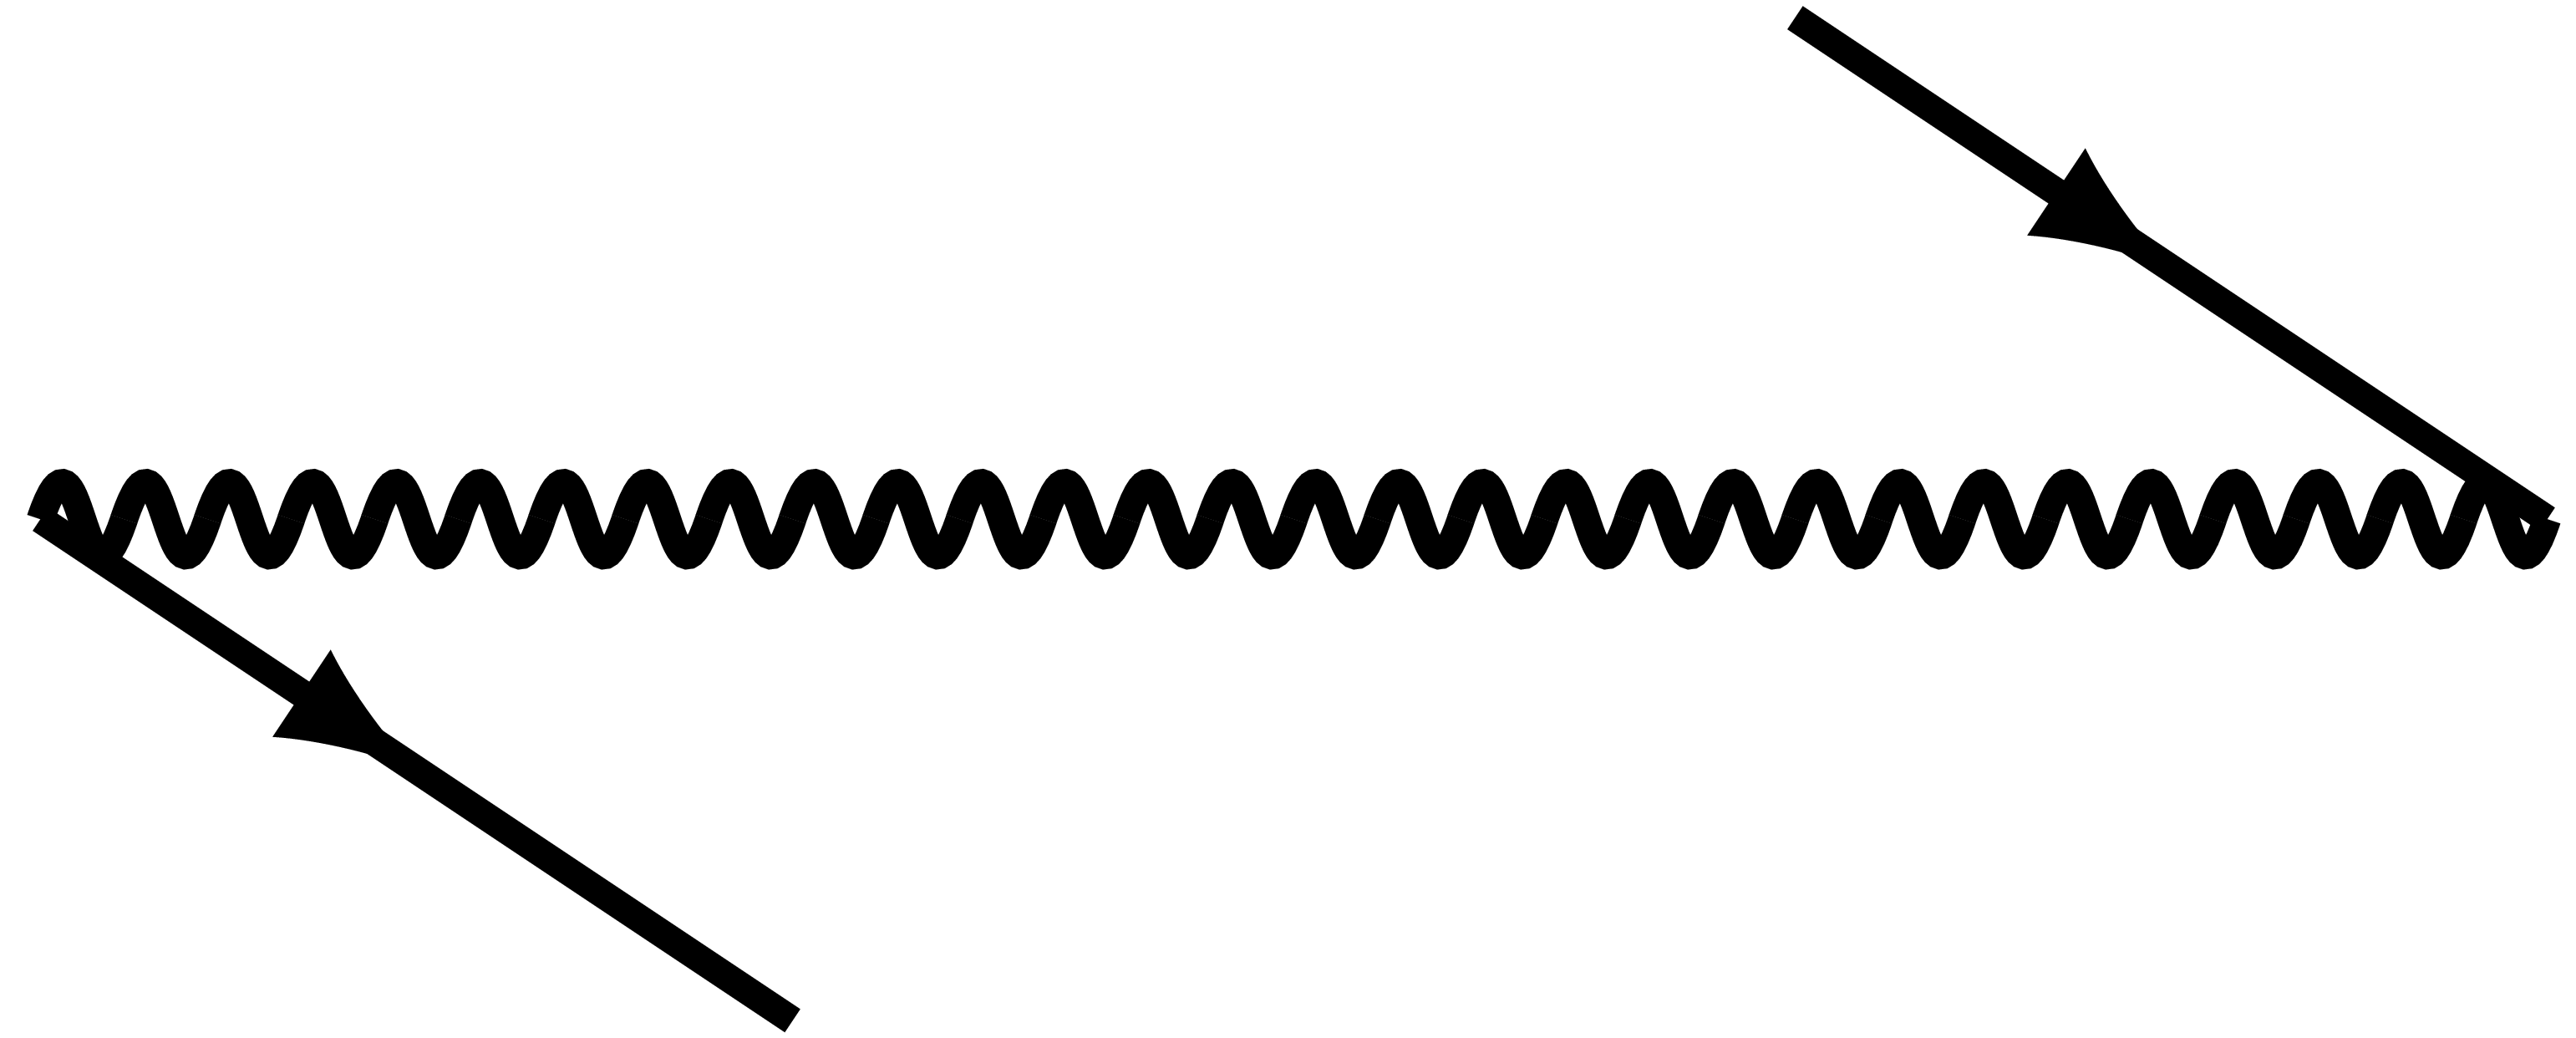
\includegraphics[align=c,width=1.2in]{EE}&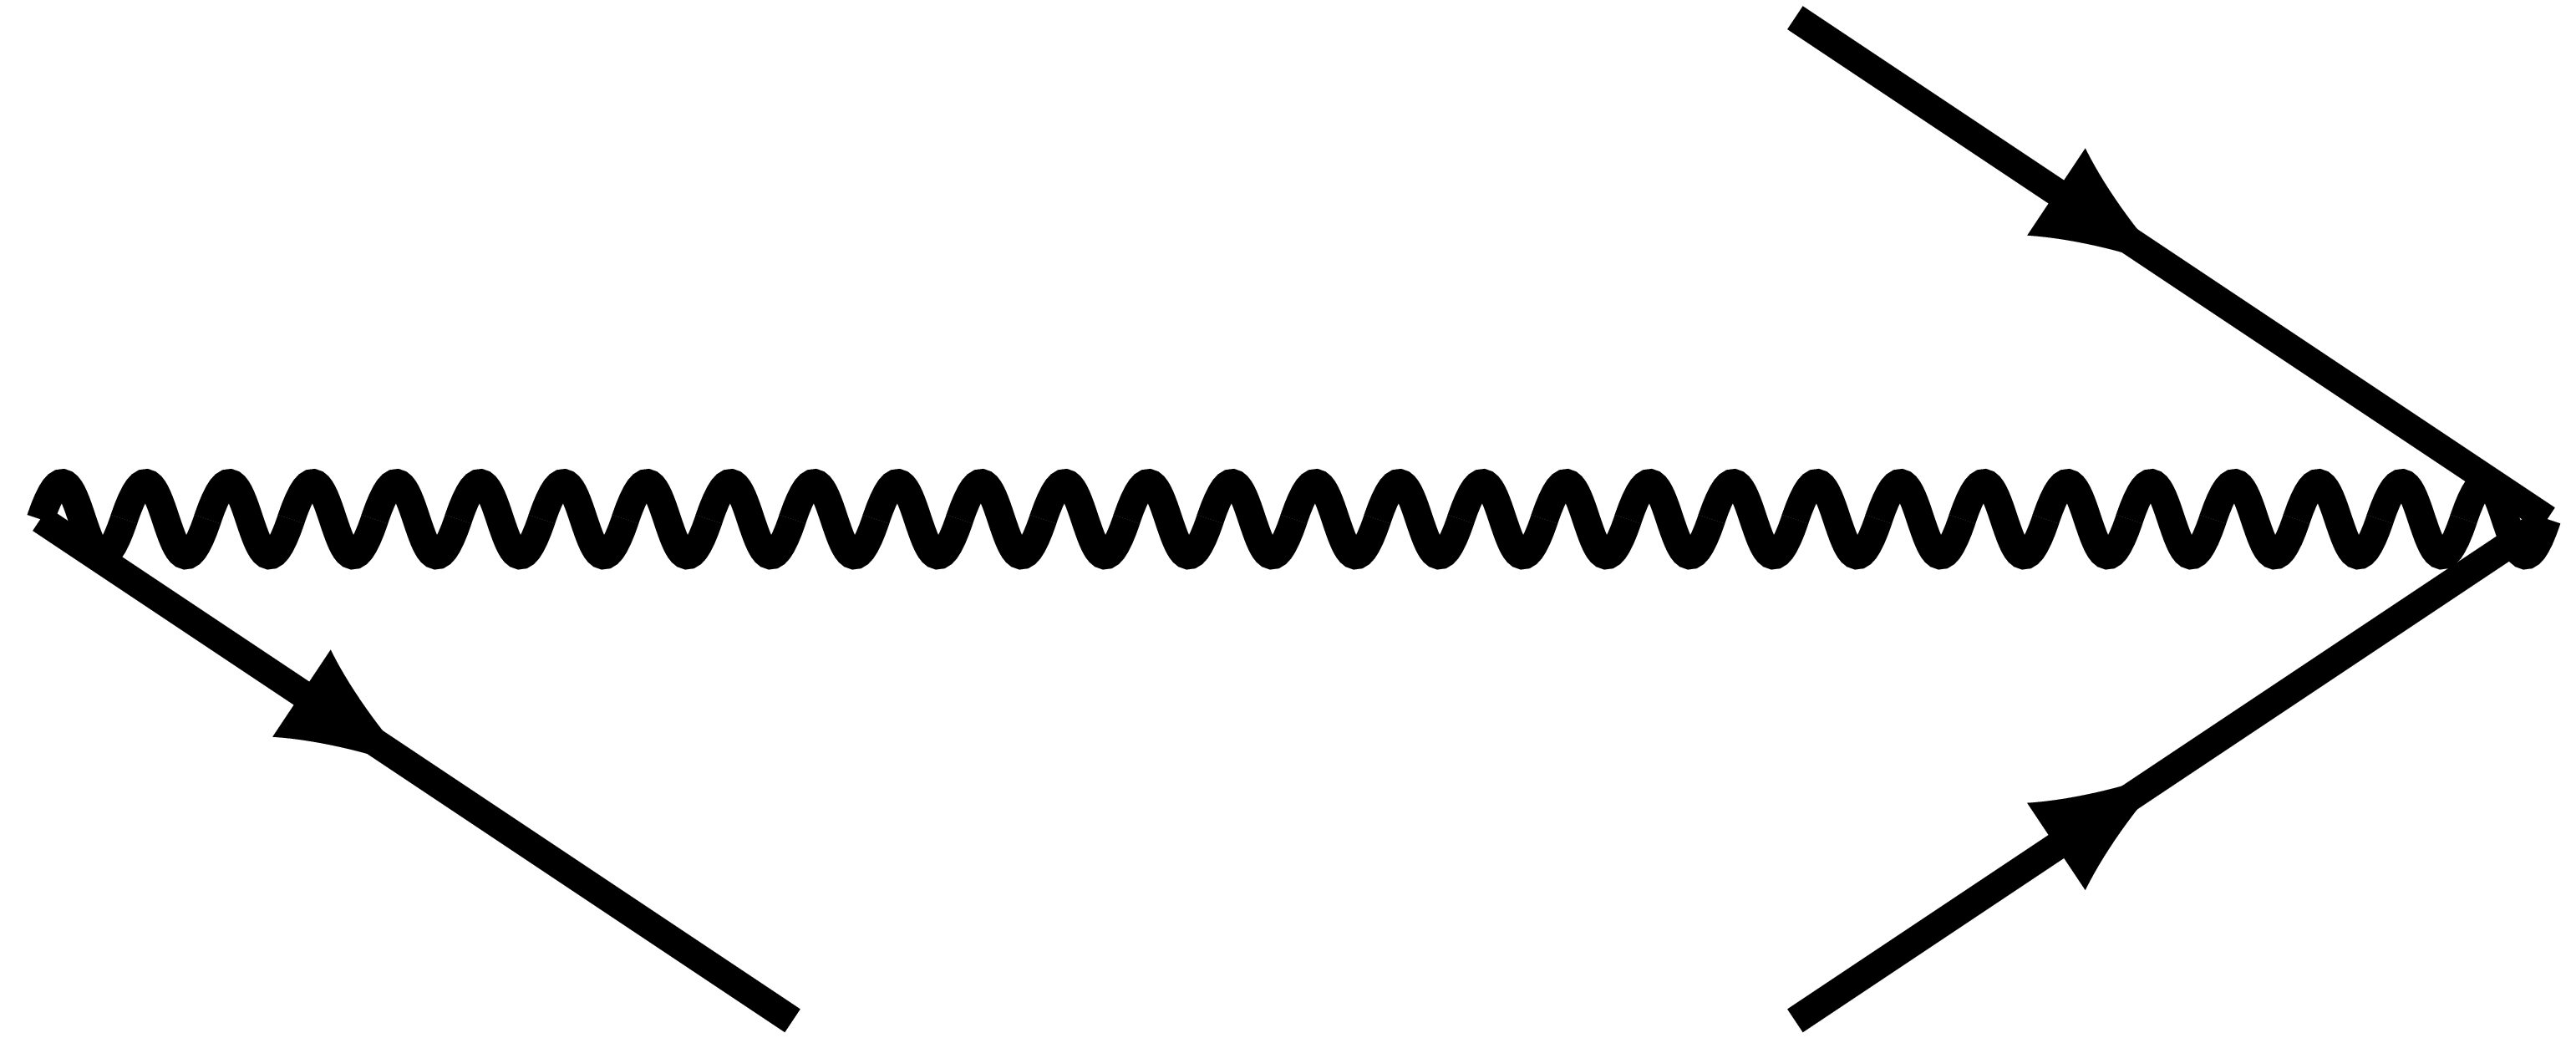
\includegraphics[align=c,width=1.2in]{EF}\\
        $F$ & 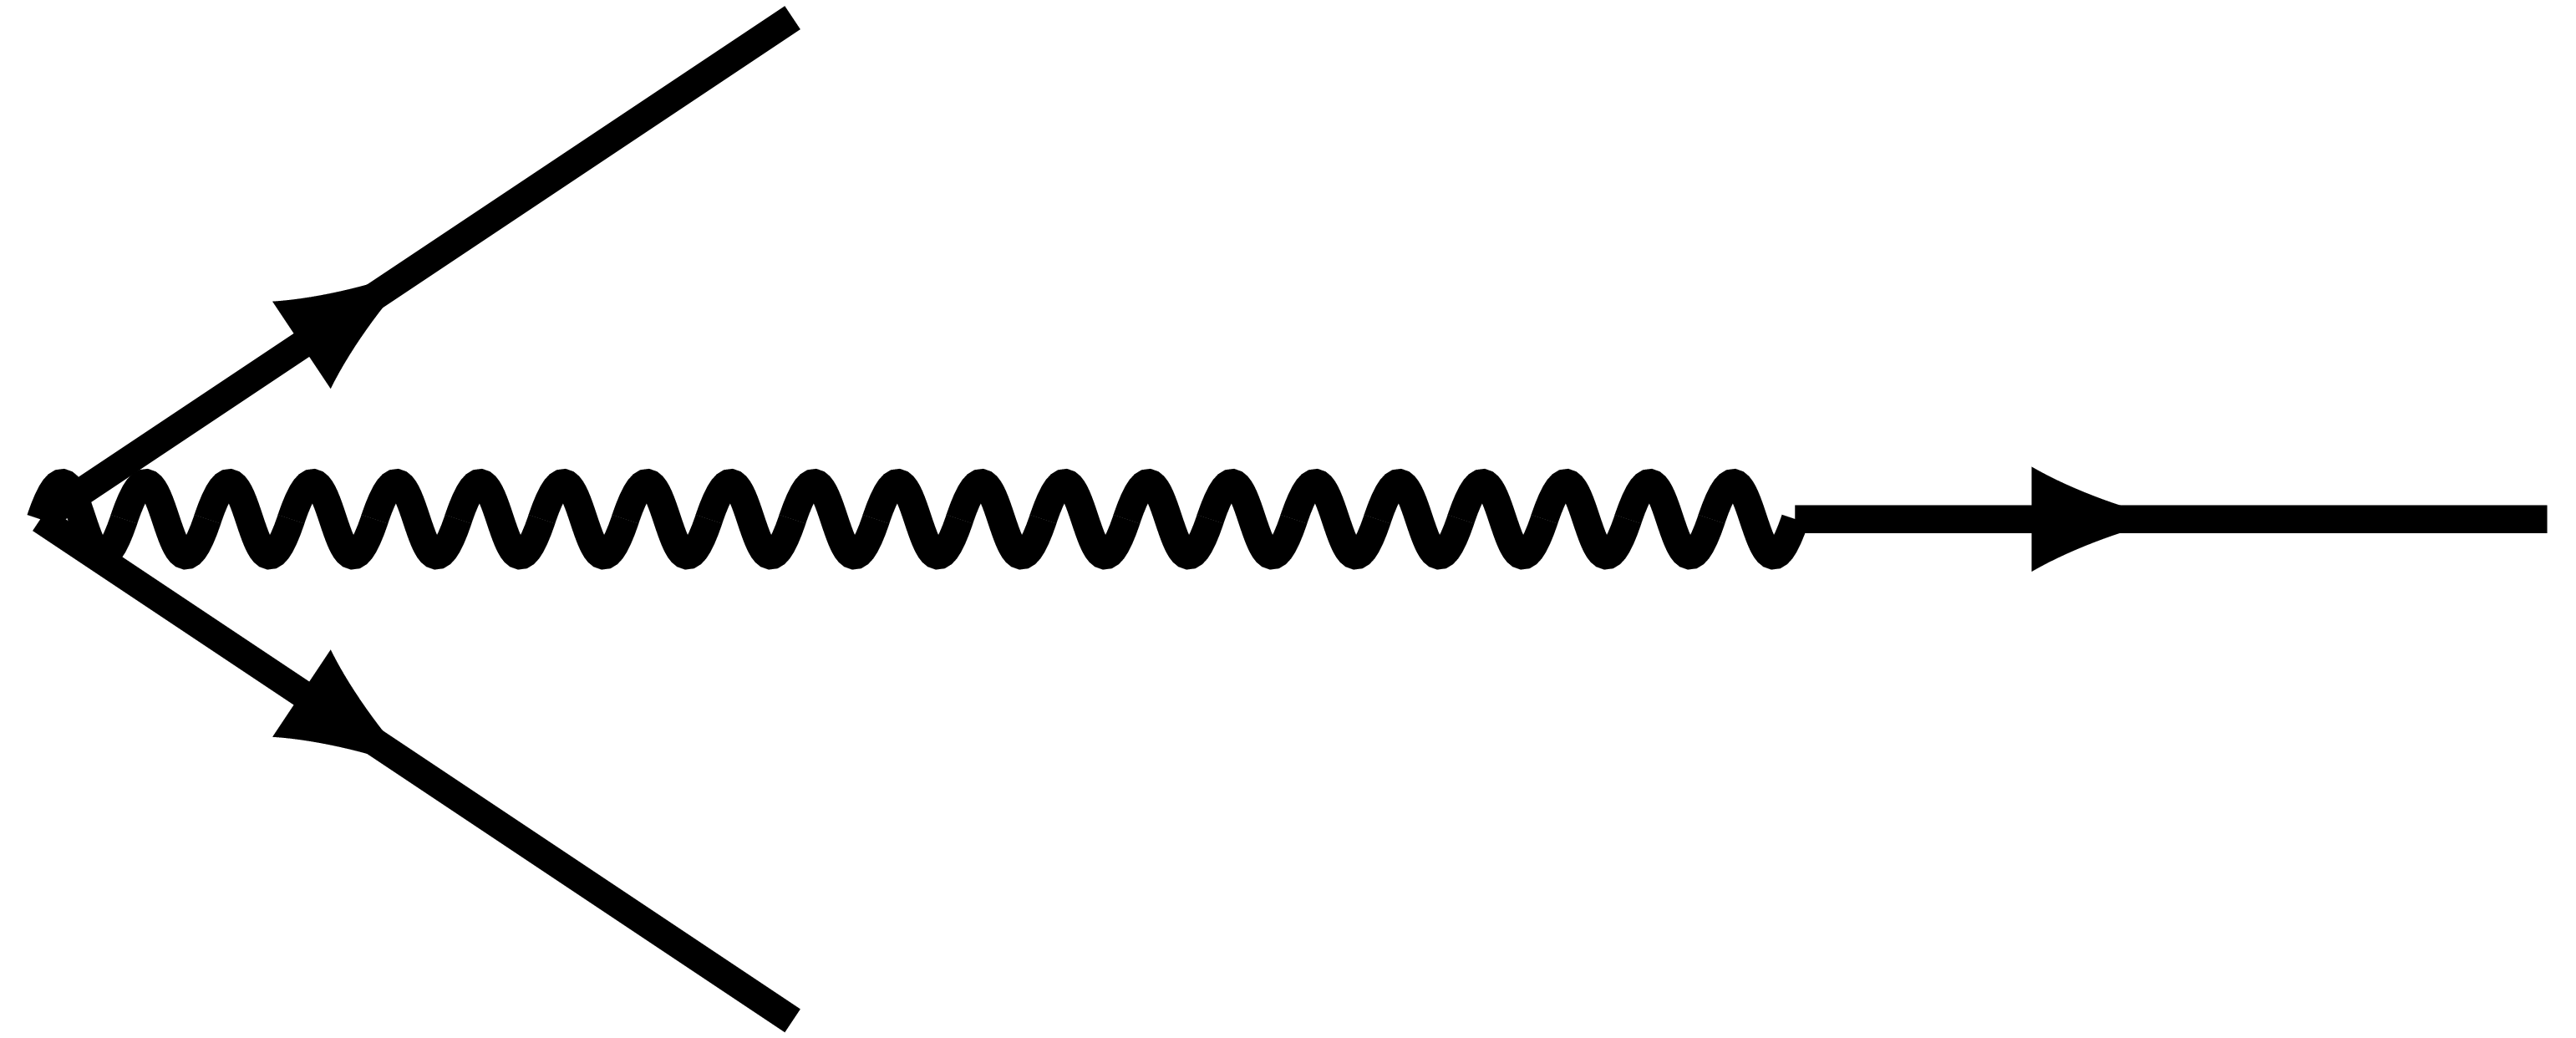
\includegraphics[align=c,width=1.2in]{FA}&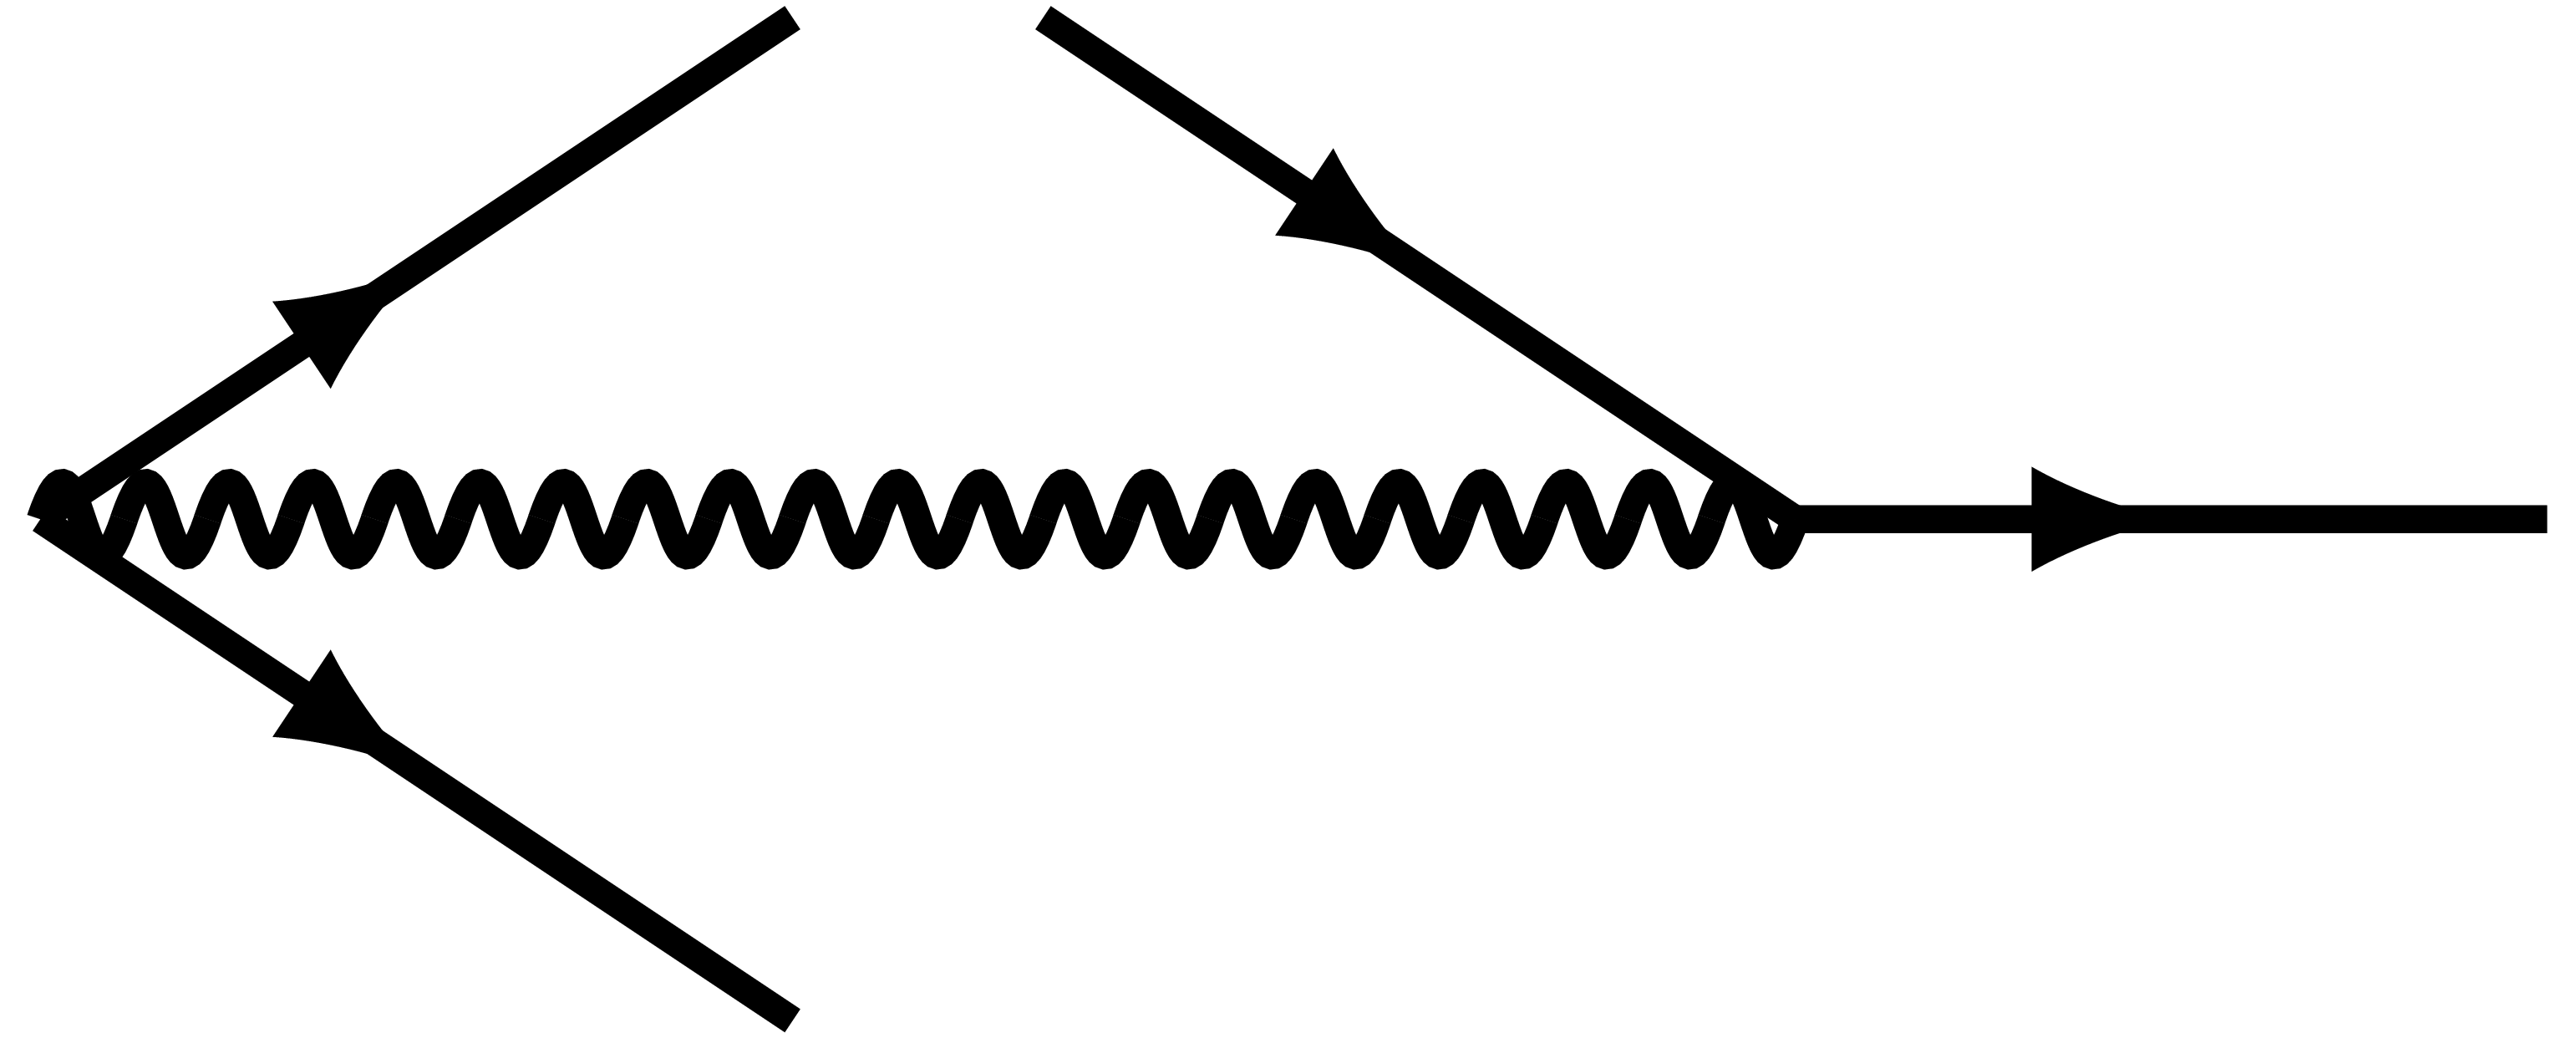
\includegraphics[align=c,width=1.2in]{FB}&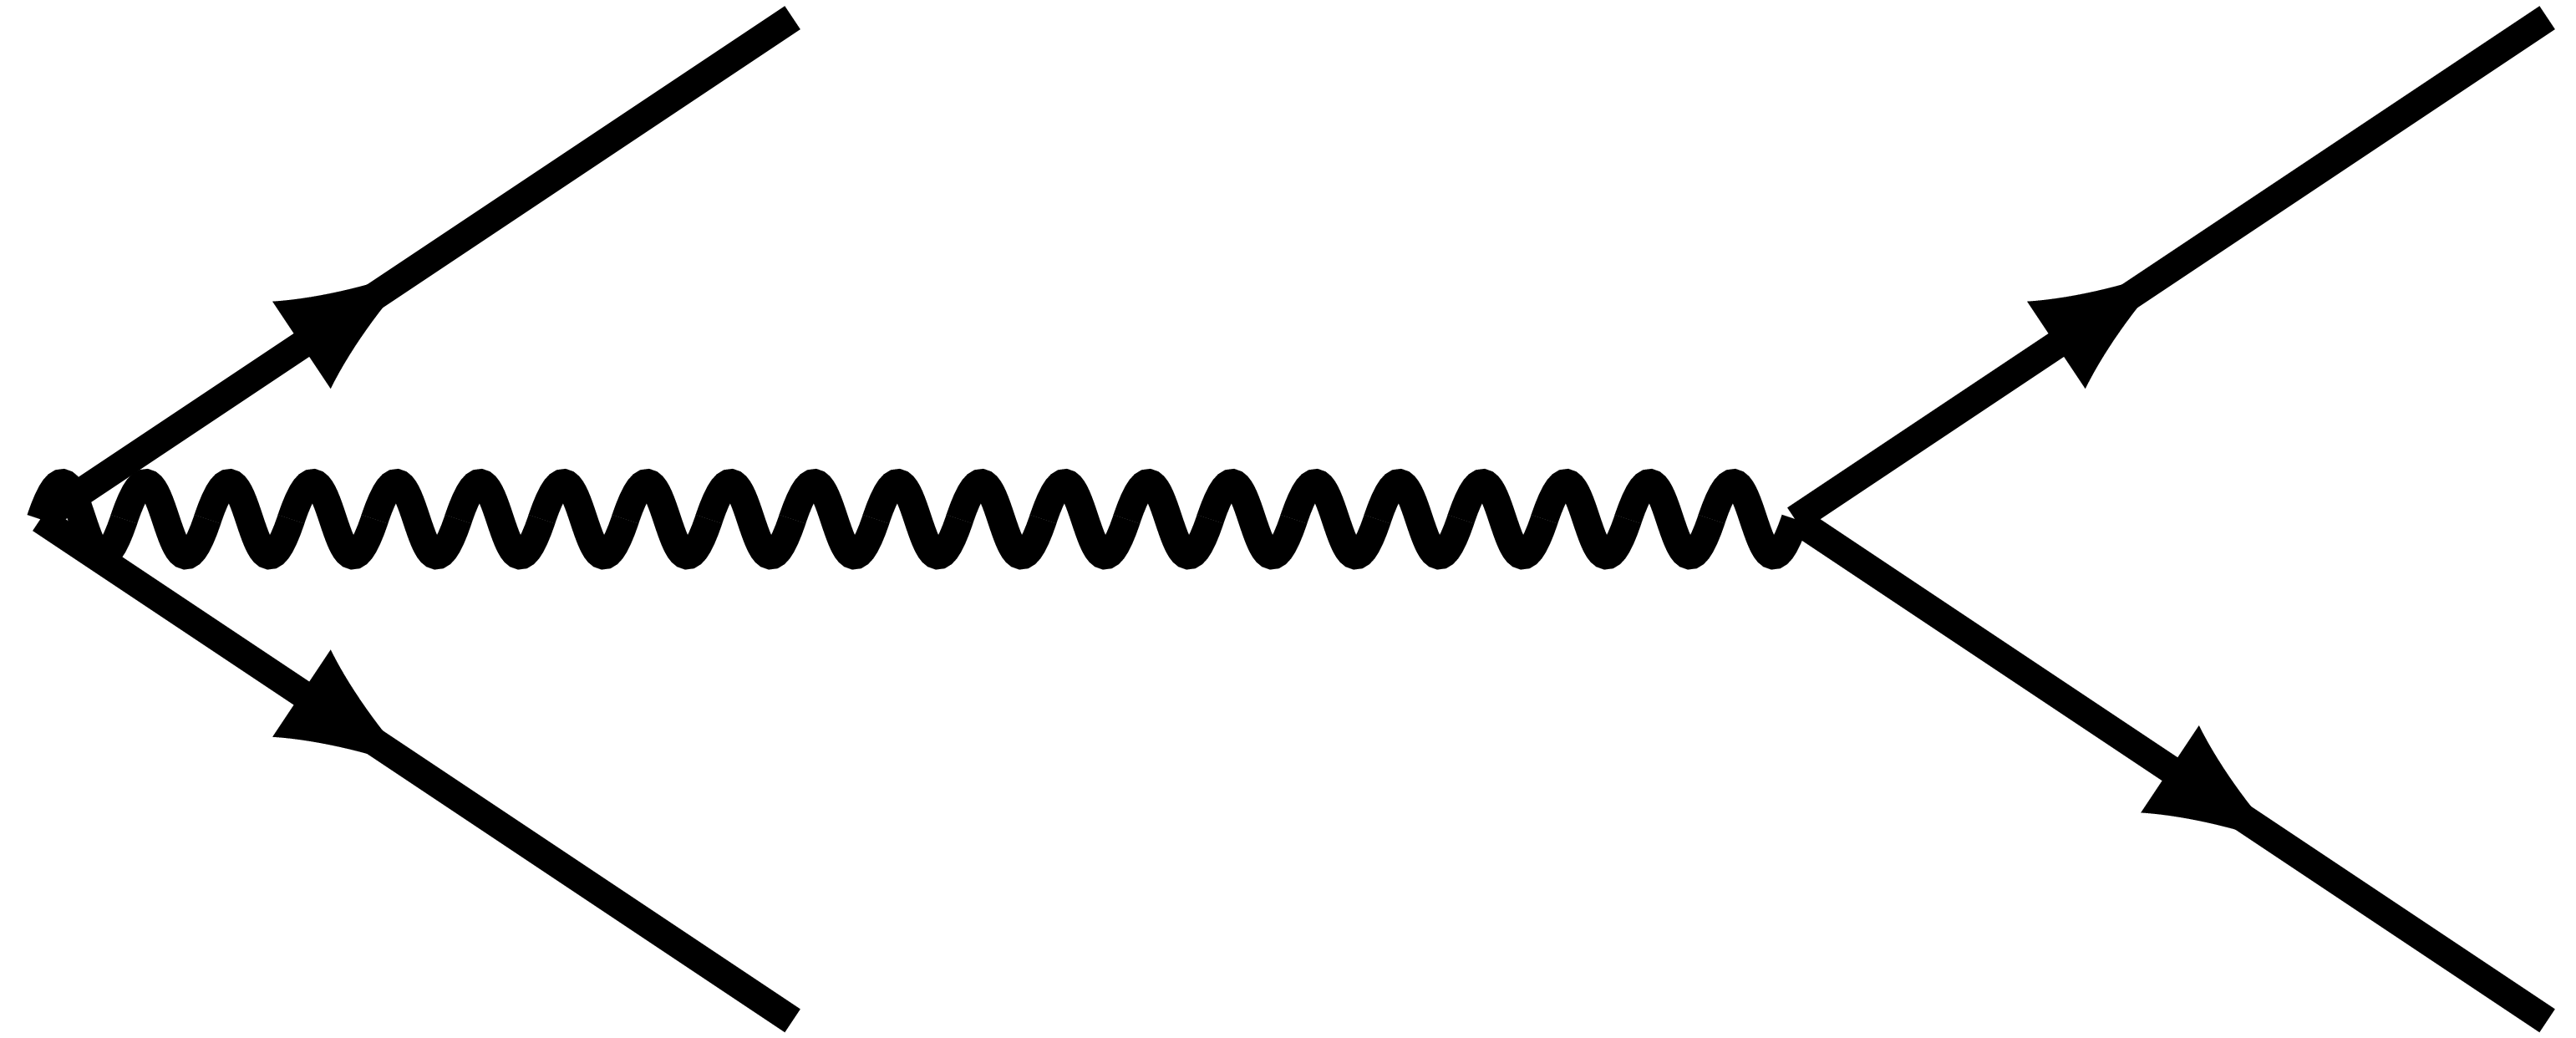
\includegraphics[align=c,width=1.2in]{FC}&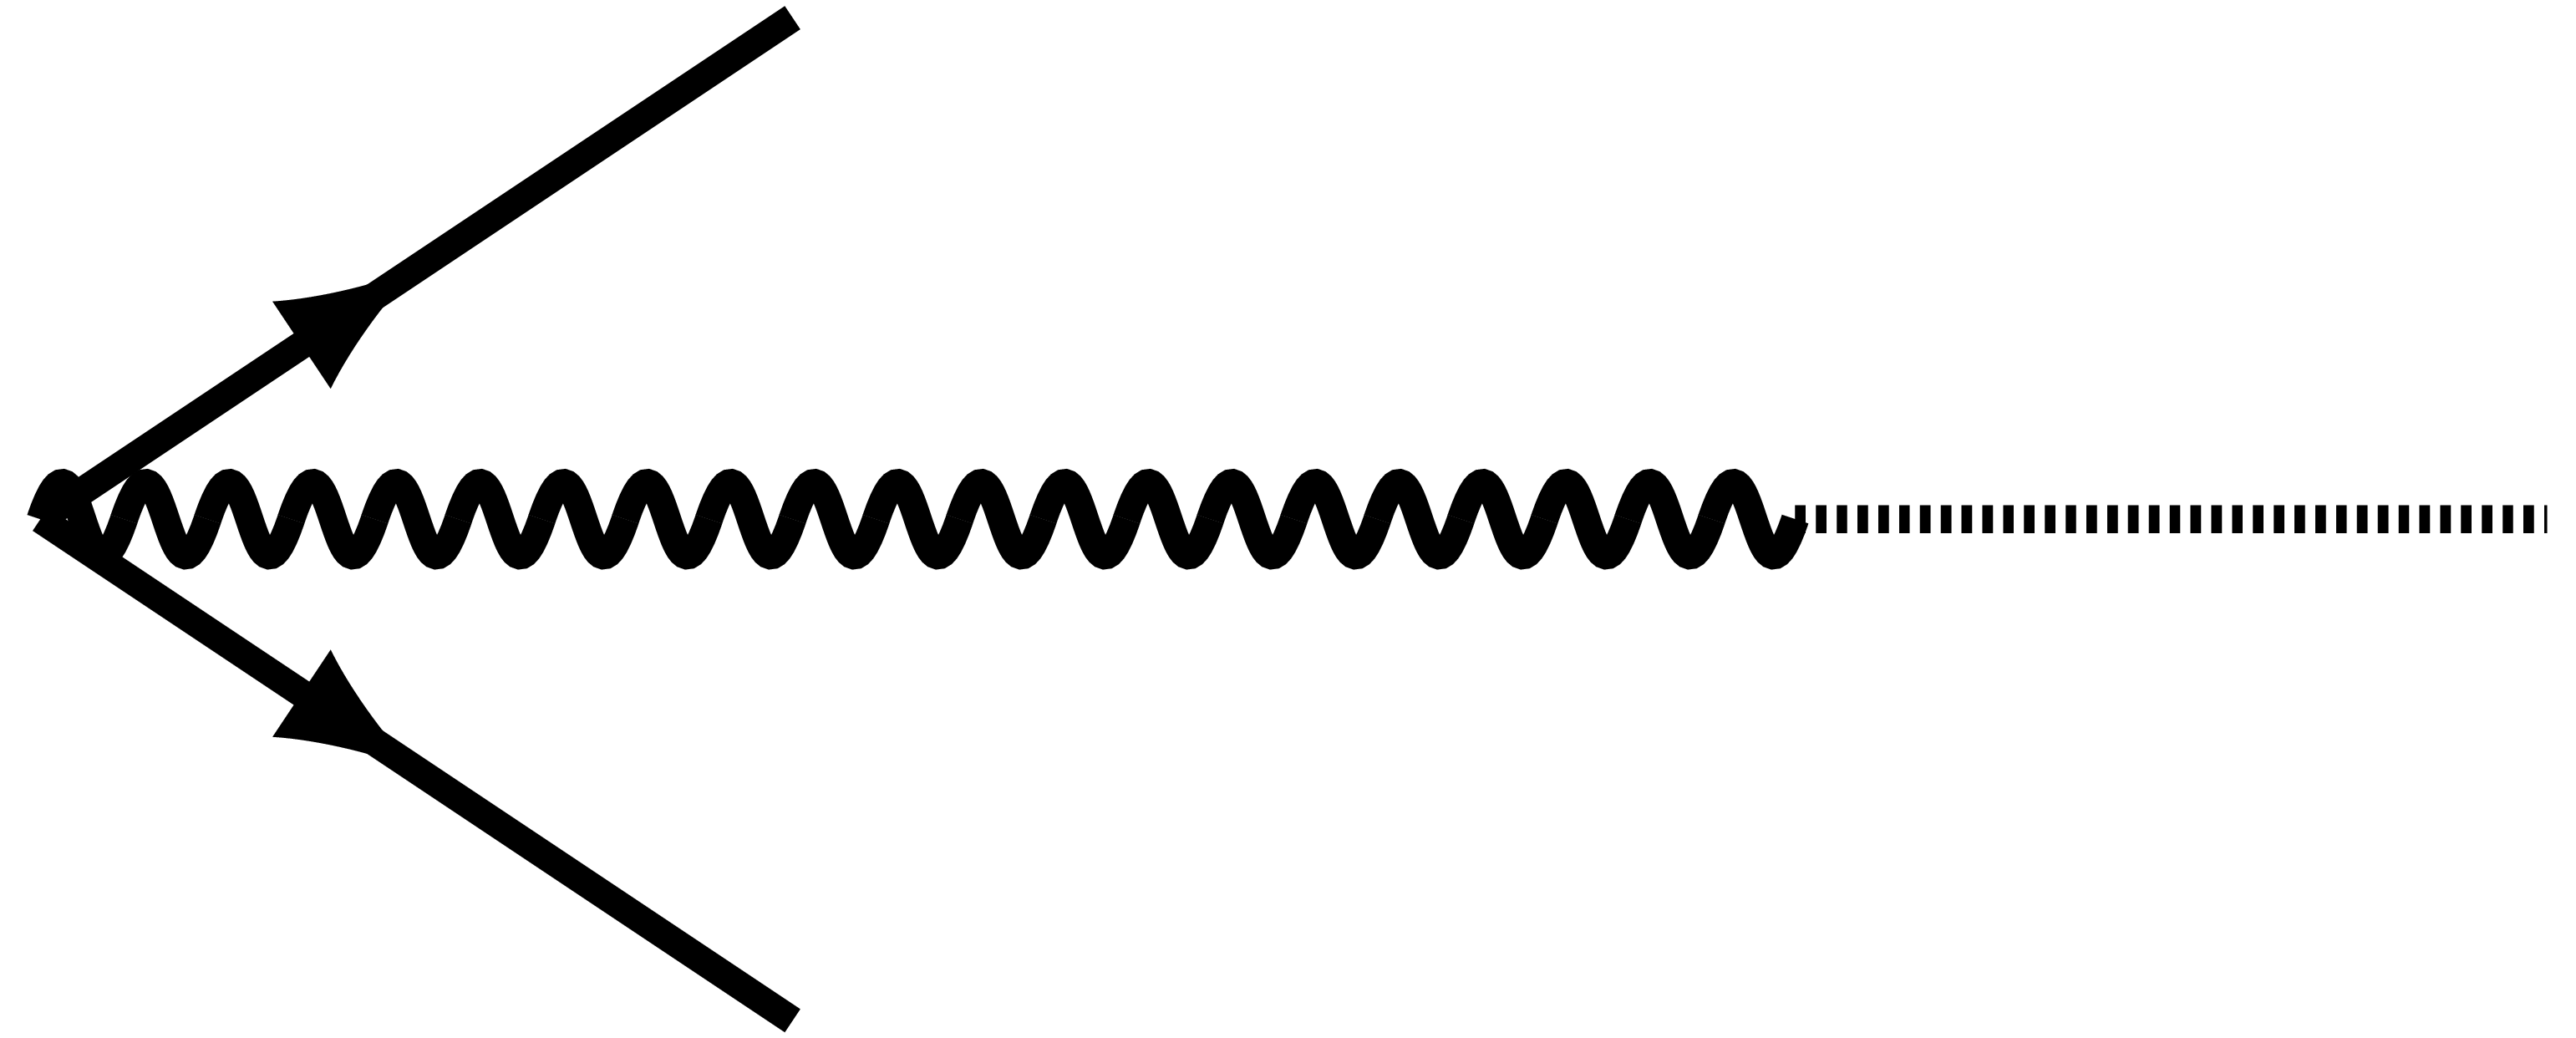
\includegraphics[align=c,width=1.2in]{FD}&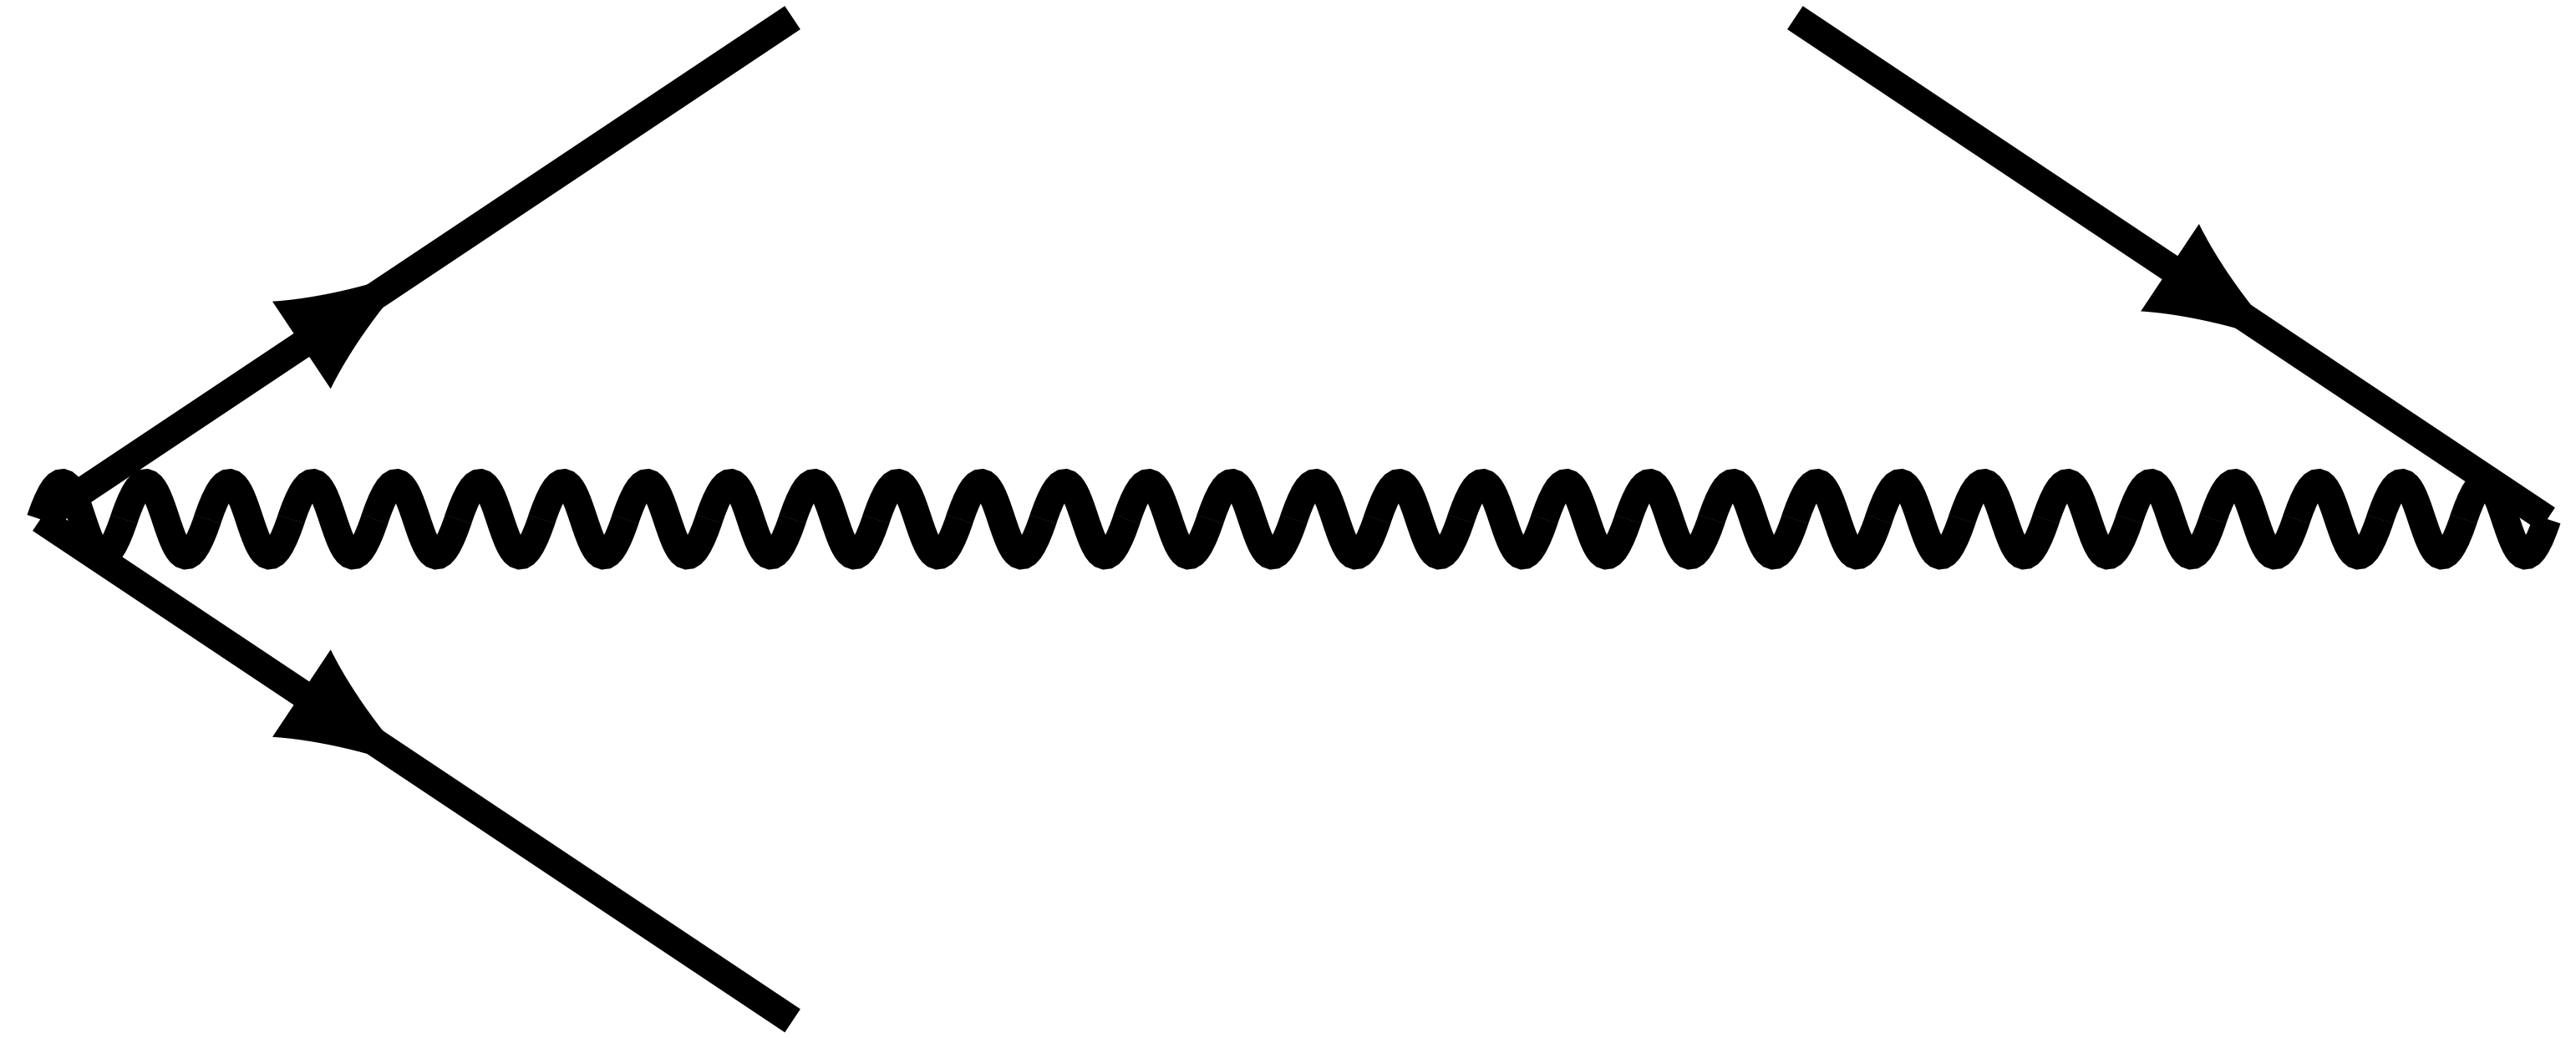
\includegraphics[align=c,width=1.2in]{FE}&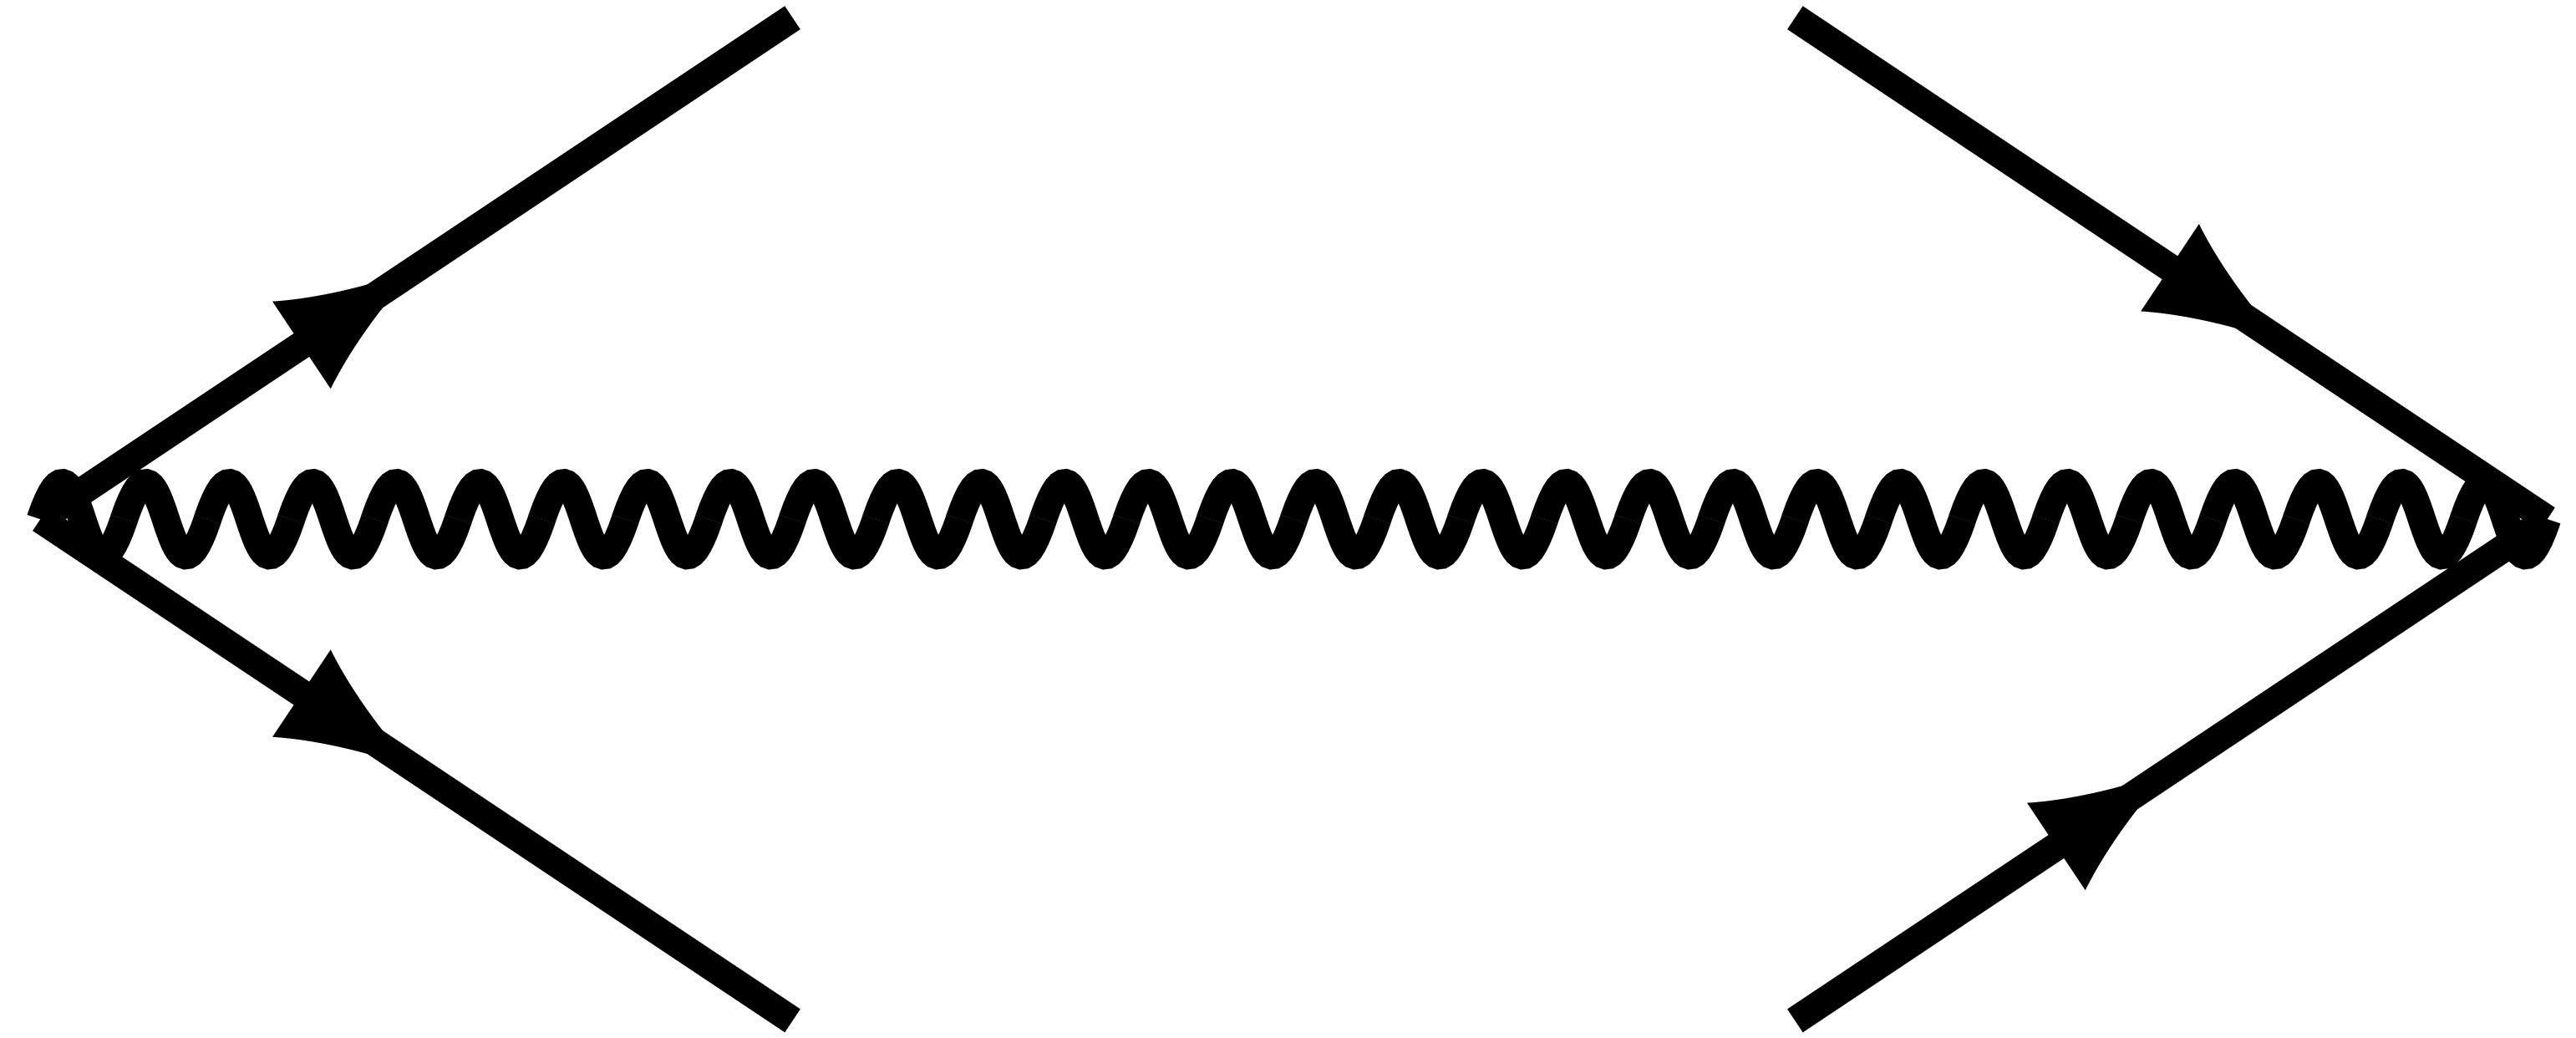
\includegraphics[align=c,width=1.2in]{FF}\\
        \end{tabular}
        \caption[Two qubit cavity coupling]{

        }
        \label{TAB:two_qubit_coupling}
    \end{table}
\end{landscape}

Table~\ref{TAB:single_qubit_diagrams} shows Feynman-like diagrams depicting the interactions between a qubit and the cavity where each diagram shows one term in the final summation in equation~\ref{EQ:cavity_hamiltonian} after expanding out the $Z_q$ in terms of the Pauli operators and the raising and lowering operators
\begin{align}
    \sigma_\pm & = \sigma_x \pm i\sigma_y     \\
    \tau_\pm   & = \tau_x \pm i\tau_y     \,.
\end{align}
The two processes labeled by $A^\dagger$ shows the creation of a photon with the relaxation of either the charge qubit ($\sigma_-$) with strength $g_\sigma$ or the spin qubit ($\sigma_z\tau_-$) with strength $g_\tau$.
Notice that the spin relaxation has a dependence on the charge state due to the presence of the $\sigma_z$.
The $B^\dagger$ processes show a spin-charge swap along with the creation of a photon.
And $C^\dagger$ shows the relaxation of both charge and spin states in order to emit a photon.
In addition to the three types of processes mentioned above, the remaining three types are non-energy conserving processes and are shown for completeness.
In the Jaynes-Cummings model, these processes are omitted since they produce the counter-rotating terms.
While the two $A^\dagger$ processes are most dominant in the first order since are the only ones that can conerve energy, at higher orders, the remaining terms can become dominant since multiple processes can combine to conserve energy through the creation and annihilation of virtual photons.

In order the obtain the effective coupling between qubits induced by the cavity, we perform a Schrieffer-Wolff transformation.
We begin by writing the interaction Hamiltonian in the slightly more useful form.
\begin{equation}
    H_{int} = \sum_q V_q  =\sum_i (g_iQ_ia^\dagger + g_i^*Q_i^\dagger a)
\end{equation}
where $\mathbf{Q}$ is a complete basis set of operators that act only on the qubit subspaces.
Here, the summation over $i$ is no longer over each qubit but rather over the set of $Q_i$ in $\mathbf{Q}$.
While in this particular system there is no direct coupling between qubits, in general, a $Q_i$ could indeed operate on multiple qubits.
We can now apply the transformation
\begin{equation}
    \tilde{H} = e^{-S}He^S
\end{equation}
where $S$ is given by
\begin{equation}
    S = \sum_i (S_ia^\dagger - S_i^\dagger a)
\end{equation}
with matrix elements
\begin{align}
    S_{i,mn}         & = -\frac{g_i Q_{i,mn}}{E_m-E_n+\hbar\omega_c}             \\
    S^\dagger_{i,mn} & = \frac{g_i^*Q^\dagger_{i,mn}}{E_m-E_n-\hbar\omega_c} \,.
\end{align}
Let us choose a basis for $\mathbf{Q}$ such that the following equation is satisfied for any $Q_i$
\begin{equation}
    \frac{\bra{m} \sum_q H_q Q_i \ket{n}}{\bra{m}Q_i\ket{n}}- \bra{n}\sum_qH_q\ket{n} = E_m-E_n = \Delta_i \,.
\end{equation}
That is, for any $m$ and $n$ where $\bra{m}Q_i \ket{n} \ne 0$, the energy difference between states $\ket{m}$ and $\ket{n}$ is a constant $\Delta_i$.
The most general of basis sets that satisfies this criteria is simply the set of matrix elements
\begin{equation}
    \mathbf{Q} = \{ \ket{m}\bra{n}:m,n \in  [1,N) \}
\end{equation}
For systems of dimension $2^N$, a more useful basis set is the set
\begin{equation}\label{EQ:Q_criteria}
    \mathbf{Q}  =\{ I, \sigma_z, \sigma_+, \sigma_-, ... \}
\end{equation}
where the ellipsis represents all tensor product combinations of the first four operators.
It is with this basis set that the diagrams in Table~\ref{TAB:single_qubit_diagrams} were generated.
Under this condition, we can write the $S_i$ as operators
\begin{align}
    S_i         & = -\frac{g_iQ_i}{\Delta_i+\hbar\omega_c}           \\
    S_i^\dagger & = -\frac{g_i^*Q_i^\dagger}{\Delta_i+\hbar\omega_c}
\end{align}
and calculate the effective Hamiltonian up to second order in the Schrieffer-Wolff transformation.
\begin{equation}
    \tilde{H}_{int} = \frac{1}{2}\sum_{ij}g_ig_j^*\left(\frac{1}{\Delta_i+\hbar\omega_c}+\frac{1}{\Delta_j+\hbar\omega_c}\right)\left(Q_j^\dagger Q_i + \commute{Q_j^\dagger}{Q_i}a^\dagger a\right)
\end{equation}
Where the summation over $i$ and $j$ are over all of the various diagrams.
Due to the energy difference in the denominators, we must restrict ourselves to the dispersive regime where the cavity is not in resonance with the qubits.
A key feature to notice here is the case of multi-qubit coupling.
If $Q_i$ and $Q_j$ act on different qubits, they commute, and the resulting coupling does not depend on the cavity occupation.
This is consistent with the results seen in superconducting quits couples via a cavity~\cite{majer_2007}.
When $Q_i$ and $Q_j$ act on the same qubit, the commutator is not necessarily zero so the phase shift and other effects on the qubit introduced by the cavity can be dependent on the occupation number.

\section{Time Evolution}

\nocite{*}
\bibliographystyle{plain}
\bibliography{bib}
\end{document}  